\documentclass[a4paper,11pt,titlepage,twoside]{article}
\usepackage[utf8]{inputenc}

\newcommand{\Language}{CZ}
%varianty {EN} english
%         {CZ} czech
\newcommand{\Thesis}{M}
%varianty {B} bakalářská práce
%         {M} diplomová práce
%         {D} dizertační práce
\newcommand{\Faculty}{Fakulta elektrotechnická}
\newcommand{\Department}{Kybernetika a robotika}
\newcommand{\Author}{Jakub Drápela}
\newcommand{\Title}{Automatické odhadování plošek broušeného kamene}
\newcommand{\Date}{Květen 2017}
\newcommand{\Supervisor}{Ing. Vladimír Smutný, Ph.D.}

%% definice pouziteho vzoru %%%%%%%%%%%%%%%%%%%%%%%%%%%%%

\input{src/doc_head}

\usepackage{filecontents}  % create "citations.bib" on-the-fly
\begin{filecontents*}{thesis.bib}
@inproceedings{Matas,
   title = {Robust Wide Baseline Stereo from Maximally Stable Extremal Regions},
   author = {Matas, J. and Chum, O. and Urban, M. and Pajdla, T.},
   year = {2002},
   pages = {36.1-36.10},
   booktitle = {Proc. BMVC},
   isbn = {1-901725-19-7},
}
@ARTICLE{Comparison,
    author = {K. Mikolajczyk and T. Tuytelaars and C. Schmid and A. Zisserman and J. Matas and F. Schaffalitzky and T. Kadir and L. Van Gool},
    title = {A comparison of affine region detectors},
    journal = {International Journal of Computer Vision},
    year = {2005}
}
@thesis{Pohl2002,
  author       = {Petr Pohl},
  title        = {Simulace průletu paprsků transparentním objektem},
  institution  = {Czech Technical university in Prague},
  date         = 2002,
  supervisor   = {Ing. Vladimír Smutný, Ph.D.},
}
@Book{bodlakLADOK,
  author =       {Bodlák, Igor},
  title =        {Rozšíření toolboxu LADOK, Semestrální práce},
  publisher =    {Czech Technical University in Prague},
  year =         {2004},
}
@Book{strakaLADOK,
  author =       {Straka, Matěj},
  title =        {Tails of beam simulation in LADOK, Semester project},
  publisher =    {Czech Technical University in Prague},
  year =         {2013},
}
@thesis{Bodlak2005,
  author       = {Igor Bodlák},
  title        = {Modelování a analýza broušeného kamene},
  institution  = {Czech Technical university in Prague},
  date         = 2005,
  supervisor   = {Ing. Vladimír Smutný, Ph.D.},
}
@thesis{Drapela,
  author       = {Jakub Drápela},
  title        = {Měření barevných broušených kamenů},
  institution  = {Czech Technical university in Prague},
  date         = 2015,
  supervisor   = {Ing. Vladimír Smutný, Ph.D.},
}
@ARTICLE{SEXarticle,
   author = {{Bertin}, E. and {Arnouts}, S.},
    title = "{SExtractor: Software for source extraction.}",
 keywords = {METHODS: DATA ANALYSIS, TECHNIQUES: IMAGE PROCESSING, GALAXIES: PHOTOMETRY},
     year = 1996,
    month = jun,
   volume = 117,
    pages = {393-404},
   adsurl = {http://adsabs.harvard.edu/abs/1996A%26AS..117..393B},
  adsnote = {Provided by the SAO/NASA Astrophysics Data System}
}
@manual{SExtractorManual,
    author = {Bertin, E.},
    citeulike-article-id = {159020},
    citeulike-linkout-0 = {http://terapix.iap.fr/IMG/pdf/sextractor.pdf},
    keywords = {photometry, sextractor, software},
    organization = {Institud d'Astrophysique \& Observatorie de Paris},
    posted-at = {2017-03-14},
    priority = {0},
    title = {{SE}xtractor v2.5 User's Manual},
    url = {http://terapix.iap.fr/IMG/pdf/sextractor.pdf}
}
@article{PolarTrace,
author = {Katsushi Ikeuchi and Daisuke Miyazaki},
title = {Shape Estimation of Transparent Objects by Using Inverse Polarization Ray Tracing},
journal = {IEEE Transactions on Pattern Analysis \& Machine Intelligence},
volume = {29},
number = {},
issn = {0162-8828},
year = {2007},
pages = {2018-2030},
doi = {doi.ieeecomputersociety.org/10.1109/TPAMI.2007.1117},
publisher = {IEEE Computer Society},
address = {Los Alamitos, CA, USA}
}
@article{Kutulakos2008,
author="Kutulakos, Kiriakos N.
and Steger, Eron",
title="A Theory of Refractive and Specular 3D Shape by Light-Path Triangulation",
journal="International Journal of Computer Vision",
year="2008",
volume="76",
number="1",
pages="13--29",
issn="1573-1405",
doi="10.1007/s11263-007-0049-9",
url="http://dx.doi.org/10.1007/s11263-007-0049-9"
}
@book{Handbook,
 author = {Bass, Michael and DeCusatis, Casimer and Enoch, Jay and Lakshminarayanan, Vasudevan and Li, Guifang and Macdonald, Carolyn and Mahajan, Virendra and Van Stryland, Eric},
 title = {Handbook of Optics, Third Edition Volume I: Geometrical and Physical Optics, Polarized Light, Components and Instruments(Set) - chapter 12. Polarization},
 year = {2010},
 isbn = {0071498893, 9780071498890},
 edition = {3},
 publisher = {McGraw-Hill, Inc.},
 address = {New York, NY, USA}
} 
@book{HandbookDiff,
 author = {Bass, Michael and DeCusatis, Casimer and Enoch, Jay and Lakshminarayanan, Vasudevan and Li, Guifang and Macdonald, Carolyn and Mahajan, Virendra and Van Stryland, Eric},
 title = {Handbook of Optics, Third Edition Volume I: Geometrical and Physical Optics, Polarized Light, Components and Instruments(Set) - chapter 3. Diffraction},
 year = {2010},
 isbn = {0071498893, 9780071498890},
 edition = {3},
 publisher = {McGraw-Hill, Inc.},
 address = {New York, NY, USA}
} 
@url{Sarine,
  author = 		{Cut \& Symmetry Archives - Sarine},
  title = 		{Sarine - A World leading company in the diamond industry new - Sarine},
  howpublished = 	{\url{http://sarine.com/?product_category=cut-symmetry}},
  note = 		{Copyright ©2017 Sarine [cit. 17.05.2017] }
}
@url{DiaScan,
  author = 		{Sarine},
  title = 		{DiaScan S+},
  howpublished = 	{\url{http://files.jewellerynetasia.com/FileUpload/migrateddata/UserUploadImage/Showroom/Product/400/102ce128-4d0f-4402-8c92-4fb7be884d8a.jpg}},
  note = 		{JewellyNetAsia, [Online; accessed 2017-05-18], Obrázek ve formátu PNG}
}
\end{filecontents*}
\bibliography{thesis}
\addbibresource{thesis.bib}





\usepackage[export]{adjustbox}
\graphicspath{{./figures/}}
\numberwithin{table}{part}
\numberwithin{figure}{part}
\numberwithin{equation}{part}

%%%%%%%%%%%%%%%%%%%%%%%%%%%%%%%%%%%%%%%%%%%%%%%%%%%%%%%%%
\begin{document}
\shorthandoff{-}
%% uvodni stranka %%%%%%%%%%%%%%%%%%%%%%%%%%%%%%%%%%%%%%%
\TitlePage

%%% stranka s naskenovanym zadanim prace %%%%%%%%%%%%%%%%%
\thispagestyle{empty}
\begin{textblock*}{\paperwidth}(0mm,0mm)
 % \noindent\includegraphics[width=\paperwidth,height=\paperheight]{zadani.pdf}
\end{textblock*}
\mbox{}
\newpage
\thispagestyle{empty}
\begin{textblock*}{\paperwidth}(0mm,0mm)
  \noindent\includegraphics[width=\paperwidth,height=\paperheight]{zadaniBezPodpisu.jpg}
\end{textblock*}
\mbox{}
\newpage
\thispagestyle{empty}
\begin{textblock*}{\paperwidth}(0mm,0mm)
 % \noindent\includegraphics[width=\paperwidth,height=\paperheight]{zadani.pdf}
\end{textblock*}
\mbox{}
\newpage


\pagestyle{pagestyle_blue_rule}
\newgeometry{ left=4.7cm,right=3.0cm,top=3cm,bottom=4cm, twoside=false}

\pagenumbering{roman}
%% prohlaseni,podekovani,abstrakt %%%%%%%%%%%%%%%%%%%%%%%
	\newpage
	\input{src/prohlaseni}
	\newpage
	\null 
\section*{Poděkování}

Zde bych chtěl poděkovat za podporu při tvorbě této bakalářské práce. Poděkování patří především mému vedoucímu Ing. Vladimíru Smutnému, Ph.D. za poskytnuté konzultace, vstřícnost, ochotu a trpělivost. 

Dále bych rád poděkovat rodině za podporu během studia. Nemalé díky patří také přátelům za silnou morální podporu a rady, které mi pomohly tuto práci realizovat.   

\vfill{}
	\newpage
	\section*{Abstrakt}
Tato práce se zabývá automatickým odhadem orientace faset broušeného kamene s využitím informace o šíření rovnoběžného světelného svazku brusem. Důležité jsou světelné svazky vystupující z kamene. 

Metoda odhadu parametrů faset spočívá v porovnání svazků ze simulace a z měřicího experimentu. Parametry simulovaného modelu jsou upravovány gradientním optimalizačním algoritmem. Výstupem měřicího experimentu je snímek s obrazy svazků.

 První část je zaměřena na detekci světelných stop v obraze a výpočet parametrů odpovídajících svazků. Detekce stop je založena na přítomnosti maximálně stabilních extrémních oblastí (MSER) v obraze. Druhá část obsahuje návrh algoritmů k nalezení korespondujících dvojic svazků.   

Práce je zaměřena na broušený kámen typu šatonová růže s 12-ti bočními fasetami.

\textbf{Klíčová slova:} počítačové vidění, MSER, sledování paprsků, párování světelných svazků, broušené kameny 

\section*{Abstract}

This thesis describes the automatic estimation of cut stone facet orientation with the use of information about  the parallel light beam propagation. Light beams leaving the stone are significant for us.

The principle of stone facet estimation is a comparison of beams from the simulation and beams from the measurement experiment. Parameters of the simulated model are modified by the gradient optimization algorithm.  The image of light beams is the output of the measurement experiment. 

The first part is focused on light beams detection and calculating the parameters of the corresponding beams. Light beams detection is based on the presence of the maximally stable extremal regions (MSER) in the image. The second part contains the light beam matching algorithms.

The work is focused on chaton rose with the twelve side facets.


\textbf{Keywords:} computer vision, MSER, ray-tracing, light beam matching, cut stones

	\newpage
%% obsah %%%%%%%%%%%%%%%%%%%%%%%%%%%%%%%%%%%%%%%%%%%%%%%%
	\tableofcontents
	\newpage
%% seznam obrazku a tabulek %%%%%%%%%%%%%%%%%%%%%%%%%%%%%	
	\listoffigures
	\newpage
	\listoftables
%	\newpage
%	\listoflistings
\restoregeometry
\clearpage

%% stranka s naskenovanym zadanim prace %%%%%%%%%%%%%%%%%
\thispagestyle{empty}
\mbox{}
\newpage

\pagestyle{pagestyle_text}
\pagenumbering{arabic}
% VLASTNI PRACE %%%%%%%%%%%%%%%%%%%%%%%%%%%%%%%%%%%%%%%%
\newpage
\chapter{Úvod}

Drahé kameny jsou lidstvem od pradávna vyhledávány.
Jsou znakem krásy, bohatství a moci. Z počátku se kameny leštily do oblých tvarů a stávaly se součástí šperků.
S vývojem civilizace se začaly drahé kameny brousit, aby se zvýraznil lom světla a lesk minerálu. Broušením vznikaly rovinné fasety. Kombinací faset s definovanou velikostí a sklonem se vyvinuly standardní tvary jako brilliant, trilliant, rosette, baguette apod. Drahé a velmi cenné suroviny jako diamant se brousí pouze ručně. Méně významné kameny jsou převážně opracovávány automatickými stroji.  

Cenu broušených kamenů určují čtyři základní parametry. Mezi ně patří čistota, barva, hmotnost a kvalita brusu. 

Čistota určuje množství příměsí v materiálu kamene. Při tvorbě krystalu mohou dále vzniknout praskliny či vzduchové bubliny.

Broušené kameny dělíme do široké řady odstínů. Barva kamene závisí jeho chemickém složení. Důležitá je jednotnost barvy celého kamene.

Hmotnost souvisí s velikostí kamene. U diamantů se hmotnost určuje v karátech a je natolik důležitá, že se v některých případech volí kompromis mezi hmotností a kvalitou brusu.

Brus je důležitá mechanická úprava kamene. Ideálně opracovaný kámen má dokonalý soulad mezi brilancí, ohněm a jiskřením. Mezi parametry hodnotící kvalitu brusu patří kvalita povrchového opracování faset. Fasety se brousí rovinnými brusnými kotouči. Broušením mohou vzniknout rýhy, škrábance, prohlubně, abraze na hranách (zbroušení přechodu mezi fasetami), povrchová oxidace a nové fasety. Kámen je třeba brousit s vysokou přesností. Každá odchylka velikosti a úhlu fasety od ideálního tvaru zhorší optické vlastnosti kamene. Orientace faset je důležitým parametrem pro zhodnocení kvality brusu.

Jedním z nástrojů ke zkoumání optických vlastností broušeného kamene je nasvícení jeho povrchu světelným svazkem. Na fasetách broušeného kamene dochází ve zjednodušeném případě k odrazu a lomu světelného svazku. Z toho důvodu se dopadající svazek roztříští na řadu světelných svazků různých tvarů. Svazky jsou definovány směrem šíření, plochou, zářivým tokem a elektromagnetickými parametry. 

Barva, čistota a kvalita brusu mají za následek změnu geometrie svazků. Ta je jednoznačným popisem broušeného kamene. Zhodnocením vystupujících svazků můžeme určit kvalitu kamene.\\ 

Tato práce navazuje na dlouhodobý výzkum v Centru strojového vnímání na katedře kybernetiky Elektrotechnické fakulty ČVUT. 

Základním kamenem je software LADOK \cite{Pohl2002} od Petra Pohla. Simulační program LADOK zavádí pro broušený kámen geometrický model ve formě konvexního mnohostěnu s rovnými fasetami. Na povrch kamene dopadá svazek nerozbíhajících se paprsků světla z definovaného směru. LADOK řeší odrazy, lomy a dělení svazků na povrchu kamene. Svazky po opuštění kamene mají definovaný směr, zářivý tok, plochu a tvar. Tento software rozšířil Igor Bodlák \cite{bodlakLADOK} o výpočet elekromagnetické vlastnosti svazků. Matematický model kamene obohatil Martin Straka \cite{strakaLADOK}. Přechody mezi fasetami modeloval jako posloupnost většího počtu menších faset s nenulovým poloměrem křivosti. 

LADOK je matematickým řešením experimentu na obr. \ref{fig:basicMeasure}. V tomto experimentu je zdrojem světla laser. Laserový svazek dopadá na broušený kámen, kde se roztříští na mnoho menších svazků. Ty jsou po opuštění kamene zachyceny na stínítku. Stínítko snímáme kamerou a získáváme obraz svazků na stínítku ve formě digitálního obrazu.  


\begin{figure}[h!]
\begin{center}
\scalebox{0.5}{ \input{xfig/stinitko.pstex_t}}
\end{center}
\caption{Nákres principu experimentu. Laser produkuje svazek světla, který dopadá na celou plochu kamene. V kameni se svazek roztříští na mnoho svazků. Svazky vystupující z kamene v horní polorovině dopadnou na stínítko. Stínítko snímá kamera. Převzato z \cite{Drapela}.}
\label{fig:basicMeasure}
\end{figure}


Experimentální soustavu máme sestavenou a zkalibrovanou \cite{Drapela}. Známe transformaci mezi obrazem svazku na stínítku a směrem, ve kterém opouští kámen. 

O možnost porovnání dat reálného experimentu s výsledky počítačové simulace se postaral Igor Bodlák \cite{Bodlak2005}. Navrhl optimalizaci kritéria hodnotící rozdíl vzdálenosti stop z experimentu a odrazů stop simulace na stínítku. Optimalizovaly se parametry faset kamene a kámen se tak deformoval, aby se dosáhlo co nejlepší shody v zadaném kritériu. Software pro řešení inverzní úlohy nazval zkratkou LAM. 

LAM byl použitelný pouze pro broušený kámen čtvercového tvaru. Z důvodu složitosti přiřazení stop z experimentu k obrazům simulovaných svazků při osvětlení celého kamene zaměřil vstupní laserový svazek pouze do určitých míst kamene. Tím vzniklo redukované množství svazků a korespondence se simulovanými svazky se výrazně zjednodušila. Nevýhodou tohoto přístupu jsou rozměry kamene, které musí být několikanásobně větší než průměr laserového svazku. Metoda je prakticky nepoužitelná pro kameny o rozměrech v jednotkách milimetru. 

	V této práci osvítíme laserovým svazkem celý kámen. Zaměříme se na kameny šatonové růže s plochým spodkem a 12-ti bočními fasetami. Tyto kameny se ve zkratce nazývají \textit{viva12}. Rozměry kamenů budou v řádech milimetrů. 
	
	K robustní detekci obrazu svazků z digitálního obrazu použijeme MSER detektor \cite{Matas}. Z výsledku detekce určíme parametry stop. Sestavíme program, pomocí kterého bude možno manuálně párovat obrazy svazků broušeného kamene se simulovanými stopami.
 Optimalizací z LAMu získáme náklony faset. Parametry svazků prozkoumáme pomocí cílených experimentů. Navrhneme algoritmus pro \textit{vivu12}, který určí automaticky orientaci faset kamene. Výstupem programu budou odchylky úhlů faset kamene od jejich ideální pozice.


















\part{Metody pro odhad tvaru kamene}

\section{Triangulace, polarizace a profilprojektor}
	3D rekonstrukce objektů je častá úloha počítačového vidění. Existuje řada sofistikovaných metod, které z~více pohledů kamer vytvoří model objektu s vysokou přesností. Většina z~po\-u\-ží\-va\-ných algoritmů není použitelná pro průhledné objekty, jako je broušený kámen. Pro odhad tvaru broušeného kamene musíme použít specializované metody, které uvažují zákony lomu a odrazu či polarizaci světla. 
	
	Kutulakos et al. \cite{Kutulakos2008} přichází s myšlenkou triangulace cesty světelného paprsku. Cestu definují pozice zdrojů světla, odrazy či lomy od rozhraní a pozice kamer. Ukazuje, za jakých podmínek lze vypočítat pozice dopadu paprsku na rozhraní zároveň s normálou tohoto elementu. 
	 
	 Miyazaki a Ikeuchi \cite{PolarTrace} vyhodnocují polarizace odraženého světla od měřeného objektu. Model objektu je určen na základě Fresnelových rovnic \cite{Handbook}. Toto měření je zdlouhavé a vyžaduje složité měřicí zařízení.    


  Pro měření a vyhodnocení brusu diamantů se komerčně využívají produkty firmy Sarine \cite{Sarine}. Optická cesta je uspořádána jako profilprojektor tzn. zdroj kolimovaného světla, kámen, kamera. Kámen se při měření otáčí okolo vertikální osy. Otáčením kamene získáme sérii mnoha snímků. Vyhodnocením snímků získáme model kaneme. 
\begin{figure}[h!]
     \centering 
     \adjincludegraphics[height=5cm,trim={0 {.2\height} 0  {.2\height}},clip]{sarin.jpg}
     %\includegraphics[height =5cm]{sarin.jpg} 

\caption[Sarine Diascan S+.]{Sarine Diascan S+. Převzato z \cite{DiaScan}.}

\label{fig:histogram relativni pohyb }

\end{figure}
  
\newpage
\section{Předchozí práce}

\paragraph{LADOK}
\hspace{1mm}

Základním nástrojem dlouhodobého výzkumu v Centru strojového vnímání na katedře kybernetiky Elektrotechnické fakulty ČVUT při zkoumání broušených kamenů je software LADOK \cite{Pohl2002} od Petra Pohla. Simulační program LADOK zavádí pro broušený kámen ge\-o\-me\-tri\-cký model ve formě konvexního mnohostěnu. Na povrch kamene dopadá svazek rovnoběžných paprsků světla homogenní intenzity a známého směru. LADOK simuluje odrazy, lomy a dělení svazků na povrchu kamene. Svazky po opuštění kamene mají známý směr, zářivý tok, plochu a tvar. Tento software rozšířil Igor Bodlák \cite{bodlakLADOK} o výpočet polarizace. Matematický model kamene obohatil Martin Straka \cite{strakaLADOK}. Přechody mezi fasetami modeloval jako posloupnost většího počtu menších faset. 

Software LADOK simuluje experiment na obr. \ref{fig:basicMeasure}. V tomto experimentu je zdrojem světla laser. Laserový svazek dopadá na broušený kámen, kde se roztříští na mnoho menších svazků. Ty jsou po opuštění kamene zachyceny na stínítku. Stínítko snímáme kamerou a získáváme obraz svazků na stínítku ve formě digitálního obrazu.  


\begin{figure}[h!]
\begin{center}
\scalebox{0.5}{ \input{xfig/stinitko.pstex_t}}
\end{center}
\caption[Schéma experimentu.]{Nákres principu experimentu. Laser produkuje svazek světla, který dopadá na celou plochu kamene. V kameni se svazek rozdělí na mnoho svazků. Svazky vystupující z kamene v horní polorovině dopadnou na stínítko. Stínítko snímá kamera. Převzato z \cite{Drapela}.}
\label{fig:basicMeasure}
\end{figure}

\newpage
\paragraph{Měřicí soustava}
\hspace{1mm}

Experimentální soustavu máme sestavenou (obr. \ref{fig: merici soustava}) a zkalibrovanou \cite{Drapela}. Výstupem experimentu je snímek s obrazy svazků. Všechny příklady snímků v této práci jsou vykresleny v invertované podobě. Z \cite{Drapela} známe transformaci mezi obrazem svazku na stínítku a směrem, ve kterém opouští kámen. 

\begin{figure}[h!]
    \centering
    \begin{minipage}[c]{0.50\textwidth}
        \centering\includegraphics[height = 12cm]{soustava2.jpg}
    \end{minipage}
    \begin{minipage}[c]{0.46\textwidth}
        \centering\includegraphics[height = 12cm]{kalib_obrazec.jpg}
    \end{minipage}
    \\
        \caption[Měřicí soustava.]{Experimentální soustava pro zachycení svazků vycházejících z kamene ozářeného laserovým svazkem. Vlevo: sestavená měřicí soustava. Zdroj laserového svazku je umístěn v horní části. Laserový svazek prochází otvorem ve stínítku a dopadá na kámen položený na podstavci. Svazky vycházející z kamene v horní polorovině dopadnou na půlkulové stínítko. Podstavec a stínítko jsou položeny na skleněné tabuli. Obraz stínítka snímá kamera. Vpravo: sestavení soustavy při kalibraci kamery. Převzato z \cite{Drapela}.}
    \label{fig: merici soustava}
\end{figure}

\newpage
\paragraph{LAM}
\hspace{1mm}

Igor Bodlák \cite{Bodlak2005} umožnil porovnání dat reálného experimentu s výsledky počítačové simulace. Navrhl optimalizaci kritéria hodnotící rozdíl vzdálenosti stop z experimentu a odrazů stop simulace na stínítku. Optimalizovaly se parametry faset kamene a kámen se tak deformoval, aby se dosáhlo co nejlepší shody v zadaném kritériu. Software pro řešení inverzní úlohy nazval zkratkou LAM. 

LAM byl použitelný pouze pro broušený kámen čtvercového tvaru. Z důvodu složitosti přiřazení stop z experimentu k obrazům simulovaných svazků při osvětlení celého kamene se v LAMu zaměřil  vstupní laserový svazek pouze do určitých míst kamene. Tím vzniklo redukované množství svazků a korespondence se simulovanými svazky se výrazně zjednodušila. Nevýhodou tohoto přístupu jsou rozměry kamene, které musí být několikanásobně větší než průměr laserového svazku. Metoda je prakticky nepoužitelná pro kameny o rozměrech v jednotkách milimetru. 

\paragraph{Příspěvek práce} 
\hspace{1mm}

 	V této práci osvítíme laserovým svazkem celý kámen. Zaměříme se na kameny šatonové růže s plochým spodkem a 12 bočními fasetami. Tyto kameny se ve zkratce nazývají \textit{viva12}. Rozměry kamenů budou v řádech milimetrů. 
	
	K robustní detekci obrazu svazků z digitálního obrazu použijeme MSER detektor \cite{Matas}. Z~výsledku detekce určíme parametry stop. Sestavíme program, pomocí kterého bude možno manuálně párovat obrazy svazků broušeného kamene se simulovanými stopami.
	
 Optimalizací z~LAMu získáme náklony faset. Parametry svazků prozkoumáme pomocí cílených experimentů. Navrhneme algoritmus pro \textit{vivu12}, který určí automaticky orientaci faset kamene. Výstupem programu budou odchylky úhlů faset kamene od jejich ideální pozice.




 
 
 
 \clearpage
 
\part{Fyzikální model}

\section{Model kamene}
Broušený kámen je modelován jako konvexní mnohostěn \cite{Pohl2002}. Brusné kotouče považujeme za dokonale rovinné. Uchycení kamene při broušení zjednodušíme na absolutně tuhé bez známek pružnosti či ohybu. Fasety potom můžeme modelovat jako rovinné plochy. Orientace a umístění fasety získáme z výkresu nebo předchozího měření. 

Přechody mezi fasetami jsou v ideálním případě ostré hrany. Z důvodu abraze hran v procesu výroby kamene jsou hrany obroušeny do přibližně oblého tvaru. K přiblížení modelu reálnému obroušení hran aproximujeme hranu množstvím rovinných faset se vzájemnou polohou odpovídající poloměru křivosti hrany.  
  
\begin{figure}[htps]
\centering
\includegraphics[width=0.5\linewidth]{edge_ex.pdf}
\caption{Detail aproximace přechodu mezi fasetami.}
\label{fig: edge}
\end{figure}  

\section{Model svazku}
Svazek světla v LADOKU reprezentuje nerozbíhající se konvexní hranol. Vlivem odrazu a lomu se konvexní tvar zachová. Fasety jsou také konvexní, proto se konvexita zachová i při štěpení svazku. Po opuštění kamene jsou svazky definovány zářivým tokem, plochou a směrem, které lze vyjádřit pomocí azimutu a elevace. Stokesovy koeficienty definují polarizaci svazku \cite{bodlakLADOK}. 

Zaznamenána je celá cesta svazku. V každém bodě trasy známe směr a tvar svazku vyjádřený pomocí polygonu. 

Model nepostihuje situace, při kterých dochází k rozbíhavosti světla.
\begin{itemize}
\item Pokud jsou v materiálu přítomné nečistoty, praskliny, vzduchové bubliny apod., světelný svazek se rozptýlí.
\item Rozptyl světelných svazků vzniká také vlivem nedokonalého vyleštění faset, a to jak při lomu tak při odrazu.
\item Přítomnost hran v kameni způsobí ohyb světla (difrakci) \cite{HandbookDiff}.
\end{itemize}


\paragraph{Ocásky}
\hspace{1mm}

V ideálním případě lze ve snímaném obraze pozorovat pouze dopady světelných svazků, které vznikly kombinací odrazů a lomů zdrojového svazku od faset broušeného kamene. U~reálného kamene ovšem v obraze pozorujeme tenké slábnoucí přímky vycházející ze stopy světelného svazku, ocásky. Tyto ocásky vznikají díky lomu/odrazu světelného svazku od neostrých hran broušeného kamene.

\begin{figure}[h!]
\begin{center}
\scalebox{.9}{ \input{xfig/tails.pstex_t}}
\end{center}
\caption[Příklad snímaného obrazu s vyznačením obrazů svazků a ocásků.]{Příklad snímaného obrazu s vyznačením obrazů svazků a ocásků.}
\label{fig:tail_ex1}
\end{figure}


Vnik ocásků si ukážeme při lomu světla na oblé hraně kamene. Situaci budeme uvažovat v 2D prostoru, kde platí obecně stejné principy jako ve 3D. Světlo nahradíme paprsky světla se směrem šíření $\vec{v_i}$. 

Zvolíme dvě fasety svírající úhel \SI{45}{\degree}. Přechod mezi fasetami aproximujeme. Vznikne posloupnost úseček, které propojují fasety. Každé úsečce přiřadíme normálový vektor $\vec{n}$.  

\begin{figure}[h!]
\centering
\begin{minipage}[c]{0.43\textwidth}
\includegraphics[height=9cm]{edgeOutFar.pdf}
\end{minipage}
\begin{minipage}[c]{0.53\textwidth}
\includegraphics[height=9cm]{edgeInFar.pdf}
\end{minipage}

\caption[Vznik ocásků.]{Vznik ocásků na stínítku při dopadu světelných paprsků na hranu mezi fasetami \textbf{1} a \textbf{2}. Vpravo: paprsky se lomí ze skla do kamene. Vlevo: paprsky se lomí ze vzduchu do skla. Situace pro index lomu vzduchu $n_a = 1$ a index lomu skla $n_g = 1.5$.}
\label{fig:edgeIn}
\end{figure}
Aplikací Snellova zákonu a zákonu odrazu na $\vec{n}$ a $\vec{v_i}$ vypočítáme směr lomu a odrazu světelných paprsků.

Z Fresnelových rovnic \cite{Handbook} víme, že dochází nejen k lomu světla, ale část světla se odrazí. Poměr intenzity odraženého a lomeného světla závisí na polarizaci světla a dopadajícím úhlu. V této ukázce uvažujeme nepolarizované světlo. 

Na obr. \ref{fig:edgeIn} dopadají paprsky světla ze vzduchu na sklo i ze skla do vzduchu. V obou případech se odražené i lomené paprsky projeví  na stínítku jako ocásky.

Pokusíme se prozkoumat jak se mění intenzita ocásku v závislosti na úhlu $\beta$. Úhel $\beta$ uvádí absolutní úhlovou odchylku směru odraženého resp. lomeného svazku na hraně od směru odraženého resp. lomeného svazku přes fasetu \textbf{1}.  

Pro úhel $\beta$ určíme poměr intenzity ocásku $I_{\beta}$ a intenzity dopadajícího paprsku $I_0$. 
\begin{equation}
 \frac{I_\beta}{I_0}  = \frac{\rho_{{max}}}{\rho_\beta}\cdot R_\beta
\end{equation}
pro odražené paprsky a 
\begin{equation}
 \frac{I_\beta}{I_0}  = \frac{\rho_{max}}{\rho_\beta}\cdot (1-R_\beta)
\end{equation}
pro lomené paprsky, kde  

	\begin{tabular}{l l}
	$\rho_{\beta}$  & 	- hustota paprsků pro daný úhel $\beta\,$,\\
	$\rho_{{max}}$ 	&	- maximální hustota paprsků,\\
	$R_\beta$		&	- odrazivost z Fresnelových rovnic \cite{Handbook}.	 \\
	
	\end{tabular}
	\vspace{1mm}

\begin{figure}[h!]
\centering
\begin{minipage}[c]{0.48\textwidth}
\includegraphics[width=\textwidth]{edgeIn_reflection.pdf}
\end{minipage}
\begin{minipage}[c]{0.48\textwidth}
\includegraphics[width=\textwidth]{edgeIn_refraction.pdf}
\end{minipage}
\caption[Poměrná velikost intenzity ocásku případ lomu ze vzduchu do skla.]{Poměrná velikost intenzity ocásků v závislosti na úhlu $\beta$ pro případ lomu ze vzduchu do skla. Vpravo: odraz. Vlevo: lom.}
\label{fig:edgeInGraf}
\end{figure}

\begin{figure}[h!]
\centering
\begin{minipage}[c]{0.48\textwidth}
\includegraphics[width=\textwidth]{edgeOut_reflection.pdf}
\end{minipage}
\begin{minipage}[c]{0.48\textwidth}
\includegraphics[width=\textwidth]{edgeOut_refraction.pdf}
\end{minipage}
\caption[Poměrná velikost intenzity ocásku případ lomu ze skla do vzduchu.]{Poměrná velikost intenzity ocásků v závislosti na úhlu $\beta$ pro případ lomu ze skla do vzduchu. Vpravo: odraz. Vlevo: lom.}
\label{fig:edgeOutGraf}
\end{figure}

Z grafů \ref{fig:edgeInGraf} a \ref{fig:edgeOutGraf} je patrné, že ocásky budeme pozorovat různě dlouhé a z vysokou variabilitou z hlediska intenzity. 
	  
 Intenzita a délka ocásku je ovlivněna i dalšími faktory, jako je např. délka a ostrost hrany. Všechny faktory, které ovlivňují intenzitu ocásku prozatím nejsme schopni v programu LADOK zahrnout do matematického modelu, proto pro prování svazků bude užitečná především informace o směru ocásku. 
 
 \newpage
 \paragraph{Třídy svazků}
 \hspace{1mm}
 
 Svazky jsou definovány podle posloupnosti dopadových faset. Tento způsob popisu při opakovaném použití není přehledný.
 Pro lepší orientaci svazky rozdělíme do tříd a budeme pracovat pouze s názvem třídy. Rozdělení do tříd je v příloze ....  


\section{Model stínítka}
\label{sec:stinitko}
Po dopadu laserového svazku na stínítko se záření difuzně odrazí. Odrazivé vlastnosti materiálu závisí na úhlu odpadajícího světla a lze je matematicky popsat pomocí modelu zvaného BRDF (Bidirectional reflectance distribution function). Část rozptýleného světla dopadne na stínítko do okolí ostatních stop. 

%%tohle bych zařadil na později
%Laserové stopy chceme detekovat v černobílém HDR snímku půlkulového stínítka, na které dopadá část laserových svazků vystupujících z nasvíceného kamene. Snímek ze zatížen radiálním zkreslením, které je způsobeno vlastností optické soustavy objektivu. Radiální zkreslení bylo určeno v předchozí bakalářské práci \cite{Drapela}. Snímek lze pomocí transformace z \cite{Drapela} zkreslení zbavit. Z \cite{Drapela} navíc známe transformaci mezi pozicí bodu v nezkresleného snímku a odpovídajícím parametrům azimutu a elevace.


\section{Model kamery}
\label{sec:poisson}
 Použitý CCD snímač má $2050^2$ pixelů. Každému pixelu odpovídá jeden samostatný snímač, který funguje na principu počítání přicházejících fotonů po dobu expozice. Počet přicházejících fotonů v daném časovém intervalu se řídí Poissonovým rozdělením. Pravděpodobnost, že napočítáme $n$ fotonů je 
 
 \begin{equation}
    P(\mathrm{X} = n)=\frac{\lambda ^{n}\,\mathrm{e}^{-\lambda}}{n!}\,,
 \end{equation}
 kde $\lambda$ je střední hodnota a $\mathrm{X}$ náhodná veličina, která popisuje dopad fotonů na snímač. 

\clearpage








\section*{Detekce světelných stop v obraze}
Pro analýzu vlastností broušeného kamene je důležité detekovat světelné stopy vzniklé dopadem laserový svazků, vystupujících z kamene umístěného v naší experimentální soustavě, na stínítko. Zároveň je třeba určit parametry stop, které je možné porovnat s parametry svazků matematického modelu kamene v LADOKu. 

Pří zkoumání obrazu, lze intenzity pixelu rozložit na dvě základní složky. Mezi ně patří velikost pozadí a příspěvek od odpadajícího laserového svazku. Ve zjednodušeném případě lze říci, že po odečtení pozadí získáme oblasti, kde se nachází laserové stopy. Při detekci laserových stop však narážíme na řadu problémů.

Prvním problémem je určení samotného pozadí. Jednoduchou myšlenkou by bylo prahování obrazu nad konstantní úrovní. V našem obraze však pozadí typicky konstantní není. Po dopadu laserového svazku na drsné stínítko se nezanedbatelná část záření difuzně odrazí. Odrazivé vlastnosti materiálu závisí na úhlu odpadajícího světla a lze je matematicky popsat pomocí abstrakce zvané BRDF (Bidirectional reflectance distribution function). BRDF se navíc může v různých částech stínítka lišit z důvodu rozdílné koncentrace příměsí v materiálu. Odrazivost materiálu zapříčiní nárůst intenzity světla nejen v místě dopadu světelného svazku, ale i v jeho okolí. Nejznatelnější nárůst intenzity záření pozorujeme v blízkém okolí stopy. Z toho důvodu je třeba počítat s dynamicky měnící se hodnotou pozadí, která závisí především na zářivém toku, hustotě a úhlu dopadajících svazků. Rozdílné pozadí se může také vytvořit odrazem zdrojového svazku od jiných předmětů, než broušeného kamene. Hlavním příspěvkem je v tomto případě odraz od podstavce, na který pokládáme broušený kámen.

Další nepříjemnost nastává při překrývání laserových stop. Odfiltrováním pozadí získáme oblasti, kde se nachází světelné stopy. Pokud dochází k překrytí dvou či více stop nevystačíme pouze s jednoúrovňovým prahováním \cite{Drapela}, ale oblasti je třeba rozčlenit pomocí víceúrovňového prahování. V místě, kde je vysoká koncentrace svazků mohou dokonce svazky dopadnout tak blízko sebe, že splynou v jednu stopu (obr. \ref{Splynuti}). Zároveň předpokládáme, že se laserové stopy nepřekrývají příliš často abychom byli schopni určit pozadí.   

\begin{figure}[htbp]
    \centering
    \begin{minipage}[c]{0.48\textwidth}
        \centering\includegraphics[width=.6\textwidth]{pf_near.pdf}
    \end{minipage}
    \begin{minipage}[c]{0.48\textwidth}
        \centering\includegraphics[width=.6\textwidth]{pf_near2.pdf}
    \end{minipage}
    \\
        \caption[Slynutí dvou různých svazků.]{Ilustrace slynutí dvou různých svazků. V pravém i levém snímku se nachází typově stejné laserové svazky. Na levém obrázku dopadly na stínítko příliš blízko sebe. V tomto případě detekujeme pouze jednu stopu.}
        \label{Splynuti}
\end{figure}

Detekci zároveň komplikuje všudepřítomný šum a obraz je třeba filtrovat. Filtrováním snížíme šum v odraze, ale zároveň zmenšíme kontrast mezi stopami. 

Ne všechny svazky vystupující z kamene je možné detekovat. Svazky s vícenásobným odrazem postupně ztrácí zářivý tok. Po dopadu na stínítko mohou splynout se šumem a jejich detekce je prakticky nemožná. Mezi stopami s nízkým jasem se zároveň často objevují artefakty vzniklé nežádoucími optickými efekty např. interferencí, proto detekce bude často selhávat, pokud chceme rozpoznat i nepatrné stopy v obraze.



%%tohle bych zařadil na později
%Laserové stopy chceme detekovat v černobílém HDR snímku půlkulového stínítka, na které dopadá část laserových svazků vystupujících z nasvíceného kamene. Snímek ze zatížen radiálním zkreslením, které je způsobeno vlastností optické soustavy objektivu. Radiální zkreslení bylo určeno v předchozí bakalářské práci \cite{Drapela}. Snímek lze pomocí transformace z \cite{Drapela} zkreslení zbavit. Z \cite{Drapela} navíc známe transformaci mezi pozicí bodu v nezkresleného snímku a odpovídajícím parametrům azimutu a elevace.

\begin{figure}[htbp]
    \centering
    \begin{minipage}[c]{0.48\textwidth}
        \centering\includegraphics[width=.7\textwidth]{pf_punch2.pdf}
    \end{minipage}
    \begin{minipage}[c]{0.48\textwidth}
        \centering\includegraphics[width=.7\textwidth]{pf_deff2.pdf}
    \end{minipage}
    \\
        \caption[Problémové detekce.]{Problémové detekce. Nalevo jsou laserové stopy blízko u sebe. Stopy je nutné od sebe oddělit. Na levém snímku jsou znázorněny markantní rozdíly mezi velikostí a intenzitou stop. Je nutné použít víceúrovňový detektor. }
        \label{Detekce}
\end{figure}

\section*{Předchozí práce}

V předchozí práci \cite{Drapela} se využívalo odfiltrování pozadí obrazu a následné jednoúrovňové prahování podle intenzity. Tento přístup však nedetekoval stopy s menší intenzitou než nastavený práh a laserové stopy umístěné blízko u sebe spojil do jedné. 

Bohatší pojetí problému se objevilo v Bodlákově práci \cite{Bodlak2005}. Snímek se prahoval více než jedním prahem, přičemž z oblastí nad prahem se sestavila stromová struktura a světelné stop se určily jako listy stromu s dostatečnou významností. Tento přístup je však pro svou výpočetní náročnost nepoužitelný pro snímky s rozlišením \textit{2050x2050}, které máme k dispozici. 

Naše úloha detekce je velmi podobná detekci hvězd a galaxií v astronomických snímcích. V oblasti astronomie se hojně používá program s názvem Source Extractor \cite{SEXarticle}. Tento program má za sebou dlouholetý vývoj, je optimalizován z hlediska rychlosti a odzkoušený širokou veřejností. Tento software lze po naladění parametrů použít i pro náš případ. Nevýhodou však je, že nelze spustit operačním systémem Windows, který využíváme a neposkytuje informace o  všech oblastech, které náleží jednotlivým stopám, což je důležité pro určení parametrů laserového svazku.  

Po testu různých detektorů jsme se rozhodli pro detekci laserových stop v obraze využít relativně nový přístup uveden J.Matasem et al. \cite{Matas} v roce 2002 - MSER detektor. 

\newpage
\section*{MSER (maximal stable extremal region) detektor}

MSER detektor hledá v obraze maximálně stabilní extrémní oblasti. Původně byl využit pro robustní nalezení korespondencí mezi dvěma snímky stejného objetu pořízených z různého místa a v současné době se používá v mnoha oblastech počítačového vidění.  

Princip spočívá v několikaúrovňovému prahování obrazu podle intenzity a nalezení spojitých oblastí, které jsou nad či pod prahovou hodnotou. Mezi úrovněmi jsou nalezeny korespondující oblasti a za MSER oblasti jsou označeny ty, jejichž velikost z předchozí úrovně se se zvyšující úrovní příliš nezměnila. 

Výhodou MSER detektoru je invariance vůči afinní transformaci intenzity a vůči změně měřítka, což umožňuje současnou detekci malých a velkých oblastí s různou intenzitou. Podle studie \cite{Comparison}, která porovnává MSER detektor s ostatními typy detektorů významných oblastí, dosáhl MSER detektor skvělých výsledků v detekci oblastí s vysokou hustotu a variabilní změnou velikosti. MSER detektor se tedy zdá být vhodným kandidátem pro detekci laserových stop v obraze.

\section*{Implementace}

\subsection*{Filtrace}
   Nejprve se pokusíme z obrazu odstranit šum, který lze považovat za bílý. Šum odstraníme konvolucí s maskou, která se skládá z prvků odpovídajících Gaussově funkci. Přitom však dochází k rozmazání snímku, což může působit problémy při detekci stop. Proto pro filtraci šumu volíme kompromis, který zachová dostatečný kontrast mezi stopami a zároveň částečně odstraní šum. Pro všechny následující operace používáme místo původního snímku filtrovaný.    

\subsection*{Detekce} 
   %výstup MSER detektoru 
   Dalším krokem je detekce MSER oblastí ve filtrovaném snímku. MSER detektor je již implementován v prostředí MATLAB ve funkci \textit{detectMSERFeatures}, což zaručuje optimalizaci z hlediska rychlosti detekce. Pro aplikaci této funkce na snímek se světelnými stopami je třeba nastavit základní parametry detektoru. Mezi ně patří frekvence prahování snímku, maximální a minimální velikost MSER oblasti a dostatečná stabilita oblasti. 

\subsection*{Odstranění nežádoucích detekcí}

Výstupem detektoru je soubor MSER oblastí. U výrazné světelné stopy dostaneme data ve formě pyramidy MSER oblastí podle jednotlivých úrovní intenzity. MSER detektor však najde nejen oblasti s výrazně vyšší intenzitou, ale i oblasti s nižší intenzitou než okolí. Ty je třeba vyřadit, protože nereprezentují světelnou stopu, kterou hledáme. 

K odstranění nežádoucích detekcí použijeme následující postup. Nejdříve pro větší vyhlazení obrazu snímek rozmažeme konvolucí s Gaussovým filtrem. Následně určíme vrcholy všech MSER oblastí, což bude pixel s největší hodnotou intenzity v dané oblasti. V malém okolí vrcholů oblastí určíme průměr rozmazaného snímku. Pro efektivitu výpočtu využijeme integrální obrázek.

Spočítáme kritérium, které určuje, zda je hodnota vrcholu v rozmazaném obrázku menší než součet průměru okolí vrcholu v rozmazaném obrázku a násobku střední hodnoty intenzity nerozmazaného snímku. Ideově: 

$ HodnotaVrcholu(gauss) < \left( PrumerOkoliVrcholu(gauss) + K\times StredniHodnota(Snimek)\right)\,.$ Oblasti s vrcholy, které splňují dané kritérium odstraníme.

%\begin{itemize}
%	\item \textbf{1. Rozmazání snímku Gaussovým filtrem} - Rozmazání provedeme konvolucí snímku s poměrně velkým Gaussovým filtrem (např. 31 pixelů).
%	
%	\item \textbf{2. V okolí vrcholů najdeme průměr rozmazaného snímku} -  K tomu využíváme součet pomocí integrálního obrázku průměrujeme počtem pixelů.
%	
%	\item \textbf{3. Výpočet kritéria a odstranění vrcholu} - Kritérium pro odstranění je následující: pokud je hodnota vrcholu v rozmazaném obrázku vetší než součet průměru okolí vrcholu z rozmazaném obrázku a násobku střední hodnoty intenzity snímku. 
%	
%	Ideově: $ HodnotaVrcholu(gauss) < PrumerOkoliVrcholu(gauss) + K\times StredniHodnota(Snimek)$ . V našem případě je velikost konstanty  $ K = 0.035$.

%\end{itemize}

\subsection*{Určení pozadí snímku}
	Hodnotu pozadí potřebujeme znát, abychom ze snímku mohli extrahovat příspěvky intenzit od dopadajících laserových svazků. Určení velikosti pozadí snímku v našem případě komplikují oblasti v obraze, které nezachycují stínítko. Patří mezi ně podstavec na kámen a okolí stínítka. Zde je intenzita světla podstatně nižší, než na povrchu koule a vysoká změna intenzity komplikuje určení pozadí obrazu. Skok v intenzitě zmenšíme tak, že posuneme intenzitu pixelů v těchto oblastech na práh, který se odvíjí od střední hodnoty intenzity snímku. 
	
	Pozadí následně určíme konvolucí s Gaussovým filtrem, o velikosti řádově stovky pixelů, který ignoruje vysoké změny intenzity v obraze. Samotná konvoluce s tímto filtrem by s použitím standardní funkce \textit{conv2} byla příliš časově náročná, proto konvoluci provádíme efektivnějším způsobem, který využívá rozkladu masky filtru na singulární čísla.
	
\begin{figure}[htbp]
    \centering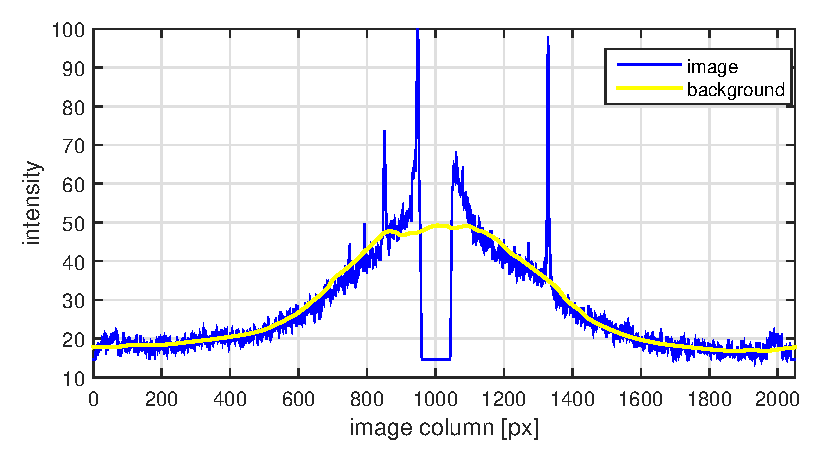
\includegraphics[width=.8\textwidth]{image_rust2.eps}
     \caption[Filtrace pozadí.]{Filtrace pozadí v HDR snímku znázorněná v řádku obrazu protínajícím obraz podstavce na kámen, který komplikuje odhad pozadí.}
        \label{fig:pozadi}
\end{figure}
	       

\subsection*{Určení vlastností laserových svazků}
Popis svazku může obsahovat tyto parametry: směr šíření svazku určený azimutem a elevací, velikost svazku, zářivý tok, intenzitu a směr světelných ocásků laserové stopy. Nově jsme si ukázali, že můžeme do popisu zahrnout velikost a směr posunu svazku při rotaci kamene. Popis svazku lze obohatit o dominantní orientaci, ke které můžeme přidat eliptický tvar stopy. 

Vlastnosti laserových svazků určíme z filtrovaného snímku, od kterého odečteme pozadí. Filtrace pozadí je znázorněna na obr. \ref{fig:pozadi}. MSER oblasti jsou roztříděny, podle toho, ke které stopě patří. Oblasti s nízkou prahovou hodnotu mohou náležet více než jedné stopě. Pro stopy   následně určíme následující parametry:

\begin{itemize}
	\item \textbf{Azimut a elevace} - Pozici světelné stopy v obraze lze určit jako polohu pixelu s maximální intenzitou v detekované oblasti. Šum v obraze ale situaci komplikuje a lepší odhad získáme, pokud určíme pozici stopy jako těžiště vrchní vrstvy pyramidy MSER oblastí příslušné stopy. Přesněji střed eliptické aproximace vrchní vrstvy. 
	
	Snímek ze zatížen radiálním zkreslením, které je způsobeno vlastností optické soustavy objektivu. Radiální zkreslení bylo určeno v předchozí bakalářské práci \cite{Drapela}, odkud navíc známe transformaci mezi pozicí bodu v nezkresleného snímku a odpovídajícím parametrům azimutu a elevace.
	
	\item \textbf{Velikost} - Pro všechny MSER oblasti určíme počet světelných stop, které se v dané oblasti nachází. Předpokládá se, že každé stopě náleží alespoň jedna MSER oblast, která obsahuje pouze tento samostatný svazek. Může ovšem nastat situace, že první vrstva pyramidy MSER oblastí, která obsahuje danou stopu, náleží také intenzivnější stopě. Méně intenzivní stopa je poté vyřazena a celá oblast přenechána významnější stopě. 
	
 	Určíme nejrozsáhlejší oblasti, které obsahují minimální počet stop a dále již počítáme pouze s nimi. U těch oblastí, které obsahují pouze jednu stopu určíme velikost a přiřadíme ji k daném svazku. Velikosti zbylých oblasti postupně dělíme podle poměru velikostí svazků před rozdělením, dokud takto nerozdělíme všechny oblasti.   
	\item \textbf{Zářivý tok} - Zářivý tok určíme obdobným postupem jako při výpočtu velikosti světelné stopy. Zářivý tok je zde součtem intenzit v dané oblasti po odečtení pozadí.   
	\item \textbf{Intenzita} - Intenzitu určíme výpočtem jako poměr zářivého toku a velikosti světelného svazku.
	\item \textbf{Orientace a eliptický tvar} -  Pro každou MSER oblast je určena elipsa, která uzavírá danou oblast. U této elipsy lze určit její orientaci. Stopa může obsahovat více MSER oblastí. Orientace stopy je určena jako medián orientací elips všech MSER oblastí a hlavní poloosy eliptického tvaru stopy jsou určeny podle MSER oblasti, která je prostřední vrstvou všech oblastí. Orientace a eliptický tvar mohou být zároveň úzce spjaty s orientací světelných ocásků.		
		
\end{itemize}

\section*{Světelné ocásky}
	V ideálním případě lze ve snímaném obraze pozorovat pouze dopady světelných svazků, které vznikly kombinací odrazů a lomů zdrojového svazku od faset broušeného kamene. U reálného kamene ovšem v obraze pozorujeme tenké slábnoucí přímky vycházející ze stopy světelného svazku (ocásky). Tyto ocásky vznikají díky lomu/odrazu světelného svazku od neostrých hran broušeného kamene. Hrany modelujeme v LADOKu jako posloupnost tenkých plošek s nenulovým poloměrem křivosti.
	
\begin{itemize}
	\item Při \textbf{odrazu} světelného svazku od hrany vzniknou v modelovém případě rovnoměrně rozmístěné svazky ležící ve stejné rovině jako svazky, které vznikly odrazem od faset propojených touto hranou.  	

	\item V případě \textbf{lomu} světelného svazku přes hranu kamene je koncentrace lomených svazků největší u svazku lomeného přes sousední fasetu kamene.  
\end{itemize}	  

\begin{figure}[h!]
\begin{center}
\scalebox{.9}{ \input{xfig/tails.pstex_t}}
\end{center}
\caption{Příklad snímaného obrazu s vyznačením svazků a ocásků.}
\label{fig:tail_ex1}
\end{figure}

	Se znalostí směru a velikosti ocásků detekovaných svazků dostáváme nové informace, které nohou přispět k jejich správnému párování se svazky z matematického modelu kamene.
	Ve snímaném obraze nelze rozpoznat všechny vznikající ocásky, ale pouze ty s dostatečně velkou intenzitou. Intenzita je přitom ovlivněna množstvím faktorů, jako je např. zářivý tok svazku, délka hrany, dopadající úhel, čistota hrany atd. Všechny faktory, které ovlivňují intenzitu ocásku prozatím nejsme schopni v programu LADOK zahrnout do matematického modelu, proto pro prování svazků bude užitečná především informace o směru ocásku. 
	
	
\section*{Detektor ocásků}
	Princip detektoru ocásků zjednodušeně spočívá v převodu okolí stopy do polárních souřadnic (vzdálenost $\rho$ a úhel $\phi$) a nalezení oblastí úhlů, ve kterých je patrný výrazný vzestup intenzity oproti okolí. Takovéto oblasti jsou typicky důsledkem přítomnosti ocásků o obraze a lze tímto způsobem ocásky detekovat. 
	
	 U rozvinutí do polárního grafu si však musíme všimnout překážek, které komplikují detekci ocásků.  
	 \begin{itemize}	 	
	 	\item V blízkém okolí jedné stopy se může nacházet další stopa. V polárním grafu se tato blízká stopa jeví jako ocásek a dochází k falešné detekci.	
	 	\item Stopy a ocásky jsou v obraze různě velké. Je třeba efektivně určovat vzdálenost $\rho$ do které budeme převádět okolí stopy do polárního grafu. Pokud zvolíme malé $\rho$ nepokryjeme oblast, kde se vyskytují ocásky a velké $\rho$ zvýší časovou náročnost výpočtu.   	
	\end{itemize}
	
	Elegantní řešení přináší použití MSER detektoru, pomocí něhož získáme vymezení oblasti a tím i vzdálenosti $\rho$, kde se stopa i s ocásky nachází. Se znalostí oblastí náležící jednotlivým stopám jsme schopni od sebe stopy částečně oddělit a redukovat množství falešných detekcí. Na druhou stranu sousední stopa muže ležet na pozici ocásku a odstraněním sousední stopy odstraníme současně i ocásek, který prozatím nejsme schopni v případě překrytí oddělit. Vzhledem k rozmanitosti stop, co do velikosti, intenzity, množství a tvaru ocásků apod. není jednoduché stopu matematicky modelovat. Pokud by se podařilo vytvořit dostatečně přesný kompaktní model stopy, je možné uvažovat o situaci, kdy budeme schopni od sebe separovat překrývající se stopy a ocásky. 
	
 Pro znázornění postupu a mezivýsledků jsme si vybrali laserovou stopu (obr.\ref{fig:mark_tail}), která v obraze nekoliduje s další výraznou stopu. Zvolená stopa vznikla dopadem laserového svazku typu ...!!doplnit(až budou popsány všechny třídy svazků)!!.... V obraze jsou patrné čtyři ocásky různě intenzity. 
	

	\begin{figure}[htp]
	\centering
	\begin{minipage}[c]{0.4\textwidth}
	\includegraphics[width=\textwidth]{figures/tail07.pdf}
	\end{minipage}
	\begin{minipage}[c]{0.4\textwidth}
	\includegraphics[width=\textwidth]{figures/tail08.pdf}
	\end{minipage}\\
	\begin{minipage}[c]{0.4\textwidth}
	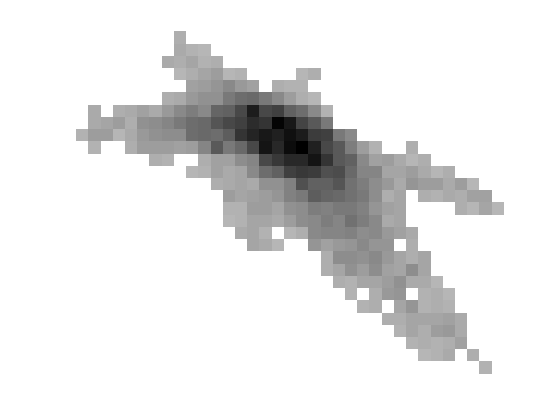
\includegraphics[width=\textwidth]{figures/tailex01.pdf}
	\end{minipage}
	\begin{minipage}[c]{0.4\textwidth}
	\includegraphics[width=\textwidth]{figures/tailex02.pdf}
	\end{minipage}
	
	\caption[Detektor ocásků - laserová stopa.]{Zvolená laserová stopa k ilustraci algoritmu detektoru ocásků. Stopa vznikla dopadem svazku typu $\dots \dots$ na stínítko. V měřicí soustavě byl přitom umístěn kámen typu \textit{VIVA $12$} s odstínem \textit{Crystal} a průměrem \SI{4.8}{\milli\meter}. Snímek vpravo nahoře znázorňuje výřez stopy ze snímaného obrazu. Můžeme zde pozorovat čtyři ocásky s různými vlastnostmi. Vlevo nahoře je výsledek detekce popsané níže. Obrázek vpravo dole ukazuje MSER oblast a poslední obrázek znázorňuje 3D pohled na zkoumanou stopu.}
	\label{fig:mark_tail}
	\end{figure}


Jednotlivé kroky algoritmu: 
	\begin{itemize}
	\item Vybereme stopu, u které chceme identifikovat ocásky a ze snímku vybereme oblast (obr.\ref{fig:mark_tail}), která náleží zkoumané stopě. 
	
	\item Po odečtení okolního šumu $z_{noise}$ prahujeme intenzitu pixelů stopy $2$krát střední hodnota intenzity $z_{mean}$. Pixely s intenzitou vyšší než zvolený práh nastavíme intenzitu odpovídající prahové hodnotě a posuneme $z_{noise}$ na hodnotu $z_{mean}$ tak, že ke všem pixelům přičteme intenzitu $z_{mean}$. Důvodem tohoto kroku je snaha odstranit nežádoucí vlastnosti velkého šumu v hodnotách intenzity v blízkém okolí "těžiště" stopy a také to, že se chceme zvětšit relativní příspěvek pixelů s nižší intenzitou do součtového kritéria \ref{eq:Isuma}.   
	
	\item Stopu s velikostí okolního šumu $z_{mean}$ převedeme do polárních souřadnic ($\rho$, $\phi$). Intenzitu $I_{pol}$ v polárním grafu $I_{pol} = f(\phi,\rho)$ určujeme pomocí bipolární interpolace, která pro větší efektivitu vynechává oblasti mimo oblast stopy, kde $I_{pol} = 0$. Důležitým parametrem při interpolaci je velikost vzorkování $f_{\phi}$ úhlu $\phi$ resp. vzorkování $f_{\rho}$ vzdálenosti $\rho$ . Experimentálně jsme zvolili $f_{\phi} = \SI{3}{\degree}$ a $f_{\rho} = \SI{1}{\px}$. Interpolaci počítáme v intervalech  $\phi \in \left\langle 0,2\pi \right\rangle$ a $\rho \in \left\langle 1,\rho_{max} \right\rangle$, kde $\phi_{max}$ je maximální vzdálenost všech pixelů v oblasti stopy od její pozice.  
	
	\begin{figure}[htbp]
    \centering
    \begin{minipage}[c]{0.48\textwidth}
        \centering\includegraphics[width=.98\textwidth]{tailex03.pdf}
    \end{minipage}
    \begin{minipage}[c]{0.48\textwidth}
        \centering\includegraphics[width=.98\textwidth]{tailex04.pdf}
    \end{minipage}
    \\
        \caption[Detektor ocásků - polární graf.]{Dva pohledy na intenzitu okolí stopy převedené do polárního grafu $I_pol$ zobrazené pomocí vrstevnic.}
        \label{Detekce}
\end{figure}
	
	\item Provedeme součet intenzit $I_{pol}$ pro jednotlivé úhly $\phi$ od minimální do maximální vzdálenosti $\rho$ a získáme závislost $I_\phi = f(\phi)$, kde  
	
	\begin{equation}
	I_{\phi_i} = \sum_{j = 1}^{\rho_{max}} I_{pol}\left(i,j\right)\,. \hspace*{2cm} i \in \left\lbrace 0, \frac{3}{180}\pi, \dots \,,2\pi \right\rbrace
	\label{eq:Isuma}
	\end{equation}
	Následně na $I_{\phi}$ aplikujeme kubickou interpolaci sousedních hodnot s $5$krát citlivějším vzorkováním $f_{\phi_2} = \frac{f_{\phi}}{5}$ a rozšíříme rozsah $\phi$ na $\phi \in \left\langle -\frac{\pi}{2},\frac{5}{2}\pi \right\rangle$. 
	
	\item Graf závislosti $I_\phi = f(\phi)$ filtrujeme konvolucí s gausiánem $g(x)$ se směrodatnou odchylkou $\sigma = 3$ a získáme referenční závislost $I_{filt}$.
	
	\begin{equation}
		g(x) = \frac{1}{\sqrt{2\pi} \cdot \sigma}e^{-\frac{x^2}{2\sigma^2}}\,.
	\end{equation}
	
	\begin{figure}[htbp]
    \centering\includegraphics[width=\textwidth]{figures/tailex05.pdf}
     \caption[Detekce ocásků - zpracování polárního grafu.]{Grafické vysvětlení funkce algoritmu pro detekci ocásků. }
    \label{fig:tailSumGraph}
	\end{figure}
	
	\item Na graf $I_{filt}$ následně opakovaně aplikujeme konvoluci, tentokrát s gausiánem $g(x)$ s vyšší směrodatnou odchylkou $\sigma = 8$, abychom získali základnu $I_{base}$, kterou budeme porovnávat se signálem $I_{filt}$.
	
	\item Nalezneme souvislé oblasti $\mathcal{R}_1, \dots , \mathcal{R}_n$, kde graf $I_{filt}$ má větší hodnotu než $I_{base}$ a sečteme rozdíly $I_{filt}$ a $I_{base}$ v jednotlivých vzorcích. Velikost součtu $S_1, \dots , S_n$ závisí na vzorkovací frekvenci $f_{\phi_2}$.
	
	\begin{equation}
	S_i = \sum_{\phi_j \colon \phi_j \in \mathcal{R}_i}I_{filt}(\phi_j)-I_{base}(\phi_j)\,. \hspace*{2cm} i \in \left\lbrace 1, 2, \dots \,, n \right\rbrace
	\label{eq:Rsuma}
	\end{equation}
	
	\item Za ocásek uvažujeme oblast $\mathcal{R}_i$, kde je součet $S_i$ větší než prahovací úroveň $s_{th}$ (pro $f_{\phi_2}$ je $s_{th} = 500$). Směr ocásku $\varphi$ je určen jako úhel, ve kterém je graf $I_{filt}$ v dané oblasti maximální a velikost ocásku $\varrho_i$ určuje $\rho_{max}$ a poměr součtu $S_i$ k maximálnímu v pro danou stopu.  
	
	\begin{equation}
	\varphi_i = \argmax_{\phi_j \colon \phi_j \in \mathcal{R}_i}I_{filt}(\phi_j) \,, \hspace{1cm} \varrho_i = \frac{S_i}{\max_{j \in 1,\dots , n}S_j}\rho_{max}\,.
	\label{eq:tail_params}
	\end{equation}
		
	\begin{figure}[htbp]
    \centering
    \begin{minipage}[c]{0.48\textwidth}
        \centering\includegraphics[width=.98\textwidth]{tail01.pdf}
    \end{minipage}
    \begin{minipage}[c]{0.48\textwidth}
        \centering\includegraphics[width=.98\textwidth]{tail02.pdf}
    \end{minipage}
    \\
        \caption[Detektor ocásků - příklad detekce.]{Ukázka funkce detektoru ocásků na vybraném vzorku z obrazu. }
        \label{Detekce}
\end{figure}


	
	
\end{itemize}	   
	
	

\section{MSER detector configuration parameter list}	
	Here is a list of the configuration parameters used for beam detection setting. All of them can be used with their default values. This description of the parameters can be usefull for understanding the algorithm or debugging.
	
\begin{center}


\begin{tabular}{l|l|p{8cm}}
    \textbf{Name} 		& \textbf{Default} & \textbf{Description} \\ \hline \hline 
    \textit{BackgroundFilt}	    	& $201$ 	& Size of Gaussian filter mask used for background estimation. \textit{Sigma} of mask is equal to \textit{BackgroundFilt} \\ \hline
    \textit{BackgroundKMean}    	& $0.15$	& $BackgroundKMean \times mean(image)$ is added to background estimation. \\ \hline
    \textit{ComputeAllLayers}   	& $1$		& $1$ - Divide all layers in marks variable calculation. $0$ - Calculate only with upper layers. \\ \hline
    \textit{ComputeTails}   		& $ 1 $		& $1$ - Tails of marks are computed. It takes some time. $0$ - No tails. Faster.\\ \hline    
    \textit{CleanerAxisRatio}   	& $ 10 $	& MSER regions with upper axis ratio are deleted. \\ \hline
    \textit{CleanerFilterSigma}  	& $ 5 $		& \textit{Sigma} of filter mask in image blurring. \\ \hline
    \textit{CleanerFilterSize}   	& $ 31 $	& Size of filter mask in image blurring.\\ \hline
	\textit{CleanerMean}    		& $ 0.035 $ & Regions with peak where difference of mean of surrounding
intensity is lower than $CleanerMean \times mean(image)$ are deleted. \\ \hline
    \textit{CleanerSumWide} 		& $ 5 $		& Size of surrounding in cleaning process.  \\ \hline
    \textit{FilterSigma}    		& $ 0.7 $	& \textit{Sigma} of niose reducing filter mask. \\ \hline
    \textit{FilterSize} 			& $ 3 $		& \textit{Size} of niose reducing filter mask.\\ \hline 
    \textit{MSERMaxAreaVar} 		& $ 0.9 $	& This value specifies the step size between intensity threshold levels used in selecting extremal regions while testing for their stability. Decrease this value to return more regions.\\ \hline
    \textit{MSERRegion} 			&$[2\,,\, 14000]$& Two-element vector, [minArea maxArea], which specifies the size of the regions in pixels. This value allows the selection of regions containing pixels between minArea and maxArea, inclusive.\\ \hline
    \textit{MSERThresh} 			& $ 1.2 $	& Increase this value to return a greater number of regions at the cost of their stability. Stable regions are very similar in size over varying intensity thresholds.\\ \hline
    \textit{SurroundThres}   		& $ 0.8 $	& Multiple of $mean(image)$ where surrounding intensity is moved.   \\ 
\end{tabular}

\end{center}

%\clearpage
\part{Parametry kamene \textit{viva12}}
\label{sec: parametryVIVA12}

Šatonová růže má 14 rovinných faset. Fasety označujeme zkratkami \textbf{TOP}, \textbf{BOT} a~\textbf{UF1-UF12}, kde

\begin{tabular}{l l}
\textbf{TOP} & - tabulka,\\
\textbf{BOT} & - spodek,\\
\textbf{UF1-UF12} & - 12 bočních faset.\\
\end{tabular}\\

Označené fasety máme na obrázku \ref{fig:viva12Params} spolu s vyznačenými parametry

\begin{tabular}{l l}
$d_{TOP}$ & průměr tabulky,\\
$d_{BOT}$ & průměr spodku,\\
$h$ & výška kamene,\\
$h_{RF}$ & výška lemu. 
\end{tabular}\\
 
Poznamenejme, že lem modelujeme množstvím faset, které po spojení aproximují oválný tvar. Tyto fasety mají v simulaci absorpční charakter. Světelné svazky, které dopadnou na lem, zaniknou.   

\begin{figure}[htps]
\centering
\begin{minipage}[c]{0.4\textwidth}
\includegraphics[width=\textwidth]{vivi12Facets1.pdf}
\end{minipage}
\begin{minipage}[c]{0.56\textwidth}
\includegraphics[width=\textwidth]{vivi12Facets2.pdf}
\end{minipage}
\caption{Šatonová růže s označenými fasetami a parametry. Pohled shora je zobrazen vlevo, bokorys vpravo.}
\label{fig:viva12Params}
\end{figure}



\clearpage





\section{Motivace a myšlenka experimentu}

Jedním z nástrojem ke zkoumání vlastností broušeného kamene je nasvícení jeho povrchu světelným svazkem. Na fasetách broušeného kamene dochází ve zjednodušeném případě k odrazu a lomu světelného svazku. Z toho důvodu se dopadající světelný svazek roztříští na řadu světelných svazků, které z kamene vystupují v různých směrech, s rozdílným zářivým tokem a dalšími typickými vlastnostmi, jako je například polarizace. 
Vystupující světelné svazky lze zachytit na stínítku. Obrazec vzniklý na stínítku jednoznačně charakterizuje broušený kámen. 

Pro tento experiment nasvícení kamene již vznikla řada programů obsahující více či méně věrohodný matematický model. Máme tedy možnost průlet světelného svazku kamenem simulovat. 

V našem případě využíváme program LADOK, který vznikl v Centru strojového vnímání na katedře Kybernetiky ČVUT v Praze. Simulační program LADOK dostatečně přesně určuje matematický model experimentu.

Cestou, jak určit tvar a další typické vlastností kamene, je rozpoznat vystupující paprsky a nalézt takový matematický model, jehož výstup by odpovídal reálné situaci (obrazci na stínítku). 

Problém však tkví v rozpoznání světelných svazků. V tomto případě jde o to ke každému svazku, viditelném na stínítku, přiřadit správnou posloupnost faset kamene, přes které se světelný svazek lomil nebo odrážel. Parametry svazku, které nám pomáhají rozpoznat jeho cestu jsou směr (azimut, elevace), zářivý tok, intenzita, plocha, velikost a směr světelných šmouh, dále nazývaných ocásky, vznikajících při průchodu světelného svazku přes hranu kamene. 

Cílem experimentu je pokusit se nalézt další parametr světelného svazku, jenž by v kombinaci s ostatními parametry pomohl svazek správně rozpoznat. 

Pokusíme se naleznout směr či velikost posunu světelných svazků při rotaci kamene nebo při naklonění zdroje dopadajícího světelného svazku. 

\newpage
\section{Popis problému}

Rotace kamene kolem osy způsobí změnu vlastností vystupujících světelných svazků (směru, zářivého toku, intenzity, vlastnosti ocásků atd.). Za určitých okolností může světelný svazek zcela vymizet. Tato situace nastává například při lomu světelného svazku z kamene do okolí. Když vlivem rotace překročíme kritický úhel, nedochází k vylomení světelného svazku, ale k totálnímu odrazu na fasetě. Světelný svazek také postupně zmizí při posunu světelného svazku mimo fasetu, a to jak při odrazu, tak při lomu. Ze stejných důvodů, proč mohou světelné svazky vymizet, mohou naopak vzniknout svazky nové.

Uvažujeme zjednodušenou situaci. Světelný svazek nahradíme světelným paprskem ležícím v jeho pomyslném těžišti. 

Světelný paprsek necháme dopadat na zrcadlo pod úhlem $\varphi_1$ a od nějž se odráží podle známého zákonu odrazu pod úhlem $\varphi_1$. Při vychýlení světelného paprsku o úhel $ \delta $ v kladném směru úhlu $\varphi_1$ je odražený úhel $\varphi_1 + \delta$. Odražený paprsek se otočí o úhel $ \delta $.

\begin{figure}[h!]
\begin{center}
\scalebox{1}{ \input{xfig/odraz2.pstex_t}}
\end{center}
\caption{Odraz laseru od zrcadla. Změna úhlu dopadajícího světelného paprsku vyvolá stejně velkou změnu úhlu odraženého paprsku.}
\label{fig:odraz laser}
\end{figure}

Jiná situace nastává při rotaci zrcadla kolem osy o úhel $\alpha$ v záporném směru. Světelný paprsek dopadá na zrcadlo pod úhlem $\varphi_1 + \alpha$. Odráží se pod úhlem $\varphi_1+\alpha$, ale vzhledem k tomu, že vstupní parsek je ve stejné pozici, se výstupní paprsek otočí o úhel  $2\alpha$. 


Důsledkem toho dostaneme identické výsledky experimentu při rotaci kamene, jako při natočení světelného zdroje o dvojnásobný úhel v opačném směru. Dále budeme tedy uvažovat pouze rotaci kamene. 

\newpage
\begin{figure}[h!]
\begin{center}
\scalebox{1}{ \input{xfig/odraz.pstex_t}}
\end{center}
\caption{Odraz laseru od rotujícího zrcadla. Rotace zrcadla vyvolá dvojnásobnou změnu velikosti úhlu odraženého paprsku.}
\label{fig:odraz zrcadlo}
\end{figure}

Pokud by docházelo pouze k odrážení od zrcadel v dvojrozměrné rovině, tak by naše zkoumání postrádalo smysl. Výstupní parsek by se vždy otočil o dvojnásobek úhlu rotace kamene, a to ve stejném směru. 

S uvažováním materiálu kamene s konstantním indexem lomu $ n_1~>~1 $ a okolí s indexem lomu $ n_2 = 1 $ se situace dramaticky mění. Vezměme si příklad lomu světelného paprsku z kamene přes rovinnou fasetu. Úhel dopadajícího paprsku na fasetu označme $\alpha_1$ a úhel lomeného svazku $\alpha_2$, pak můžeme podle Snellova zákonu psát:

\begin{center}
$n_1\,\sin(\alpha_1) = n_2\,\sin(\alpha_2) = \sin(\alpha_2)\,.$
\end{center}

\begin{figure}[h!]
\begin{center}
\scalebox{.9}{ \input{xfig/index.pstex_t}}
\end{center}
\caption{Tři případy, které mohou nastat při dopadu světelného paprsku na fasetu. Zleva lom paprsku z kamene, dopad pod kritickým úhlem a totální odraz.}
\label{fig:lom ven }
\end{figure}

Zkoumejme změnu výstupního úhlu $\alpha_2$ na změně úhlu $\alpha_1$. Nejprve si vyjádříme úhel $\alpha_2$ následně zderivujeme podle $\alpha_1$. 
\begin{eqnarray}
\alpha_2 = \arcsin(n_1\,\sin\alpha_1) \implies \frac{\mathrm{d}\alpha_2}{\mathrm{d}\alpha_1}= \frac{n_1\,\cos\alpha_1}{\sqrt{1-n_1^2\,\sin^2\alpha_1}}\,.
\label{eq:derivace uhlu}  
\end{eqnarray}

Pokud se dostáváme ke kritickému úhlu $\alpha_k$, kdy dochází k totálnímu odrazu, potom
\begin{center}
 $	\sin\alpha_2 = 1 \implies \sin\alpha_1 = \frac{1}{n_1}\,. $
\end{center}

Změnu výstupního úhlu $\alpha_2$ a vypočtením limity v okolí kritického úhlu pro $ n_1>1$ dostaneme 

\begin{eqnarray}
\lim_{n \to \alpha_k}\frac{\mathrm{d}\alpha_2}{\mathrm{d}\alpha_1} = \frac{n_1\,\cos(\arcsin\frac{1}{n_1})}{\sqrt{1-n_1^2\,\frac{1}{n_1^2}}} \to \infty\,.
\label{eq:zmena velikosti posunu}  
\end{eqnarray}
Z grafu \ref{fig:derivace uhlu} zjistíme, že minimum funkce $\frac{\mathrm{d}\alpha_2}{\mathrm{d}\alpha_1}$ vychází pro $ \alpha_1 = 0^\circ $. Po dosazení
\begin{eqnarray}
{\frac{\mathrm{d}\alpha_2}{\mathrm{d}\alpha_1}}\biggr\rvert_{\alpha_1 = 0^\circ}= \frac{n_1}{\sqrt{1-0}} = n_1\,.
\end{eqnarray}


Velikost změny posunu světelného svazku tedy může být teoreticky libovolně větší než je index lomu $n_1$. 

\begin{figure}[h!]
\begin{center}
\includegraphics[width = 8cm]{figures/derivace.eps}
\end{center}
\caption{Závislost změny lomeného úhlu na velikosti dopadajícím úhlu. Pro kritický úhel roste k nekonečnu. Graf funkce popsané vzorcem \ref{eq:zmena velikosti posunu}.}
\label{fig:derivace uhlu}
\end{figure}
\newpage


\section{Modelování pohybu světelných svazků v programu LADOKU}

V programu pro simulaci průchodu světelného paprsku konvexním objektem jsme provedli experiment s rotací broušeného kamene. Pro svoji jednoduchost jsme vybrali kámen ve tvaru šatonové růže s 12 bočními fasetami, tabulkou a spodkem ideálního tvaru (VIVA12).

Rotací kamene okolo osy kolmé ke spodku kamene dostaneme pouze soustředné kružnice. Kámen jsme tedy rotovali kolem vodorovné osy procházející středem spodku kamene o konstantní úhel v každém kroku. Zaznamenali jsme směry vystupujících svazků při různých pozicích kamene. Výsledek jsme vykreslili do polárního grafu. Ze dvou po sobě následujících pozic kamene jsme šipkou spojili pozici svazků se stejnou historií odrazu a lomů od faset kamene. Výsledný obrazec je znázorněn a grafu \ref{fig:relativni pohyb graf}.

Z praktického hlediska nás potom mohou pouze svazky, jejichž stopy lze na stínítku detekovat.

% obrazek pohybu jednotlivych stop 
\begin{figure}[h!]
\begin{center}
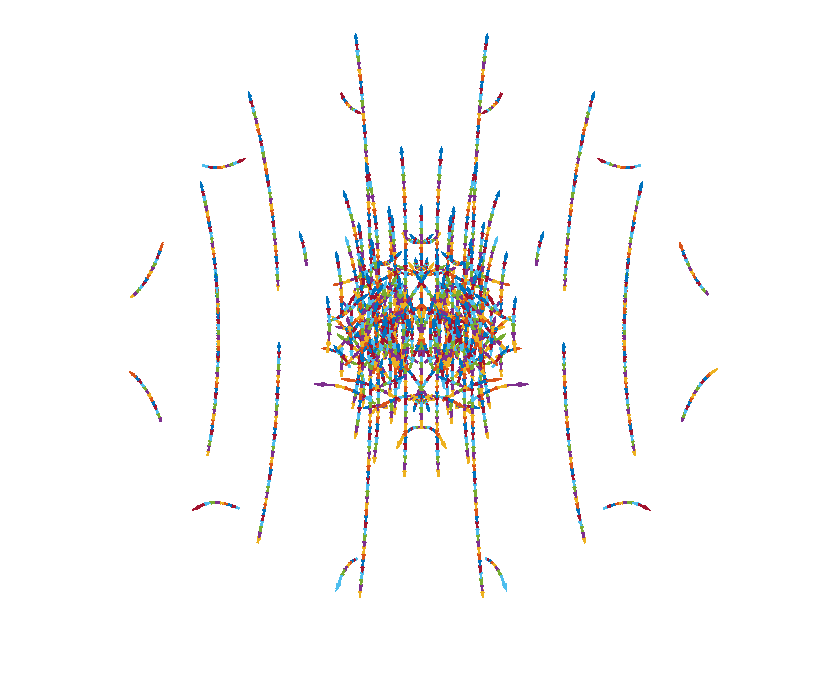
\includegraphics[width = 10cm]{figures/viva12_bigflux.eps}
\end{center}
\caption{Dráhy jednotlivých světelných stop svazků vycházejících z kamene VIVA12 získané pomocí simulačního programu  LADOK. Zobrazeny jsou pouze svazky s významnou energií vycházející v horního poloprostoru kamene. }

\label{fig:relativni pohyb graf}
\end{figure}

\newpage
Pro lepší představu o změně natočení jednotlivých svazků nám může být užitečný kruhový histogram znázorňující směr jejich pohybu (obr. \ref{fig:relativni pohyb graf}). Na něm vidíme, že větší část se pohybuje ve směru rotace kamene. Podstatná většina svazků se posouvá ve směru rotace kamene, což ovšem není příliš nápomocné při jejich identifikaci.

Existují však svazky, které jsou svým pohybem charakteristické a lze je tedy oddělit od ostatních. Kritériem pro rozpoznání svazků nemusí být pouze směr pohybu, ale jak vidíme na obr. \ref{fig:relativni pohyb graf} i velikost. V neposlední řadě přichází v úvahu i změna zářivého toku svazků, změna velikosti ocásků a další. 

\begin{figure}[h!]
 \begin{center}
 

   \begin{minipage}[c]{0.45\textwidth}
     \centering 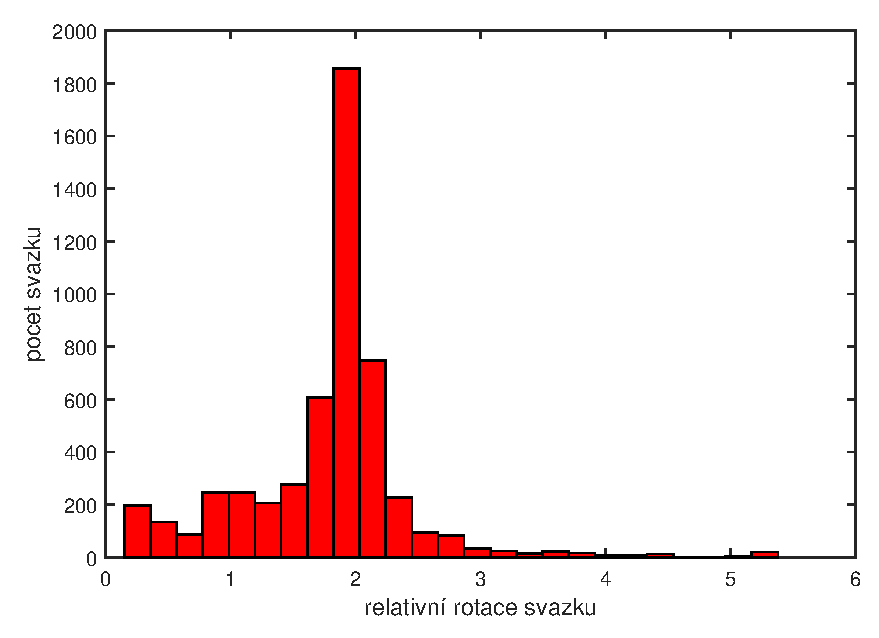
\includegraphics[height =4.5cm]{figures/relative.eps} 
   \end{minipage}
   \begin{minipage}[c]{0.45\textwidth}
     \centering 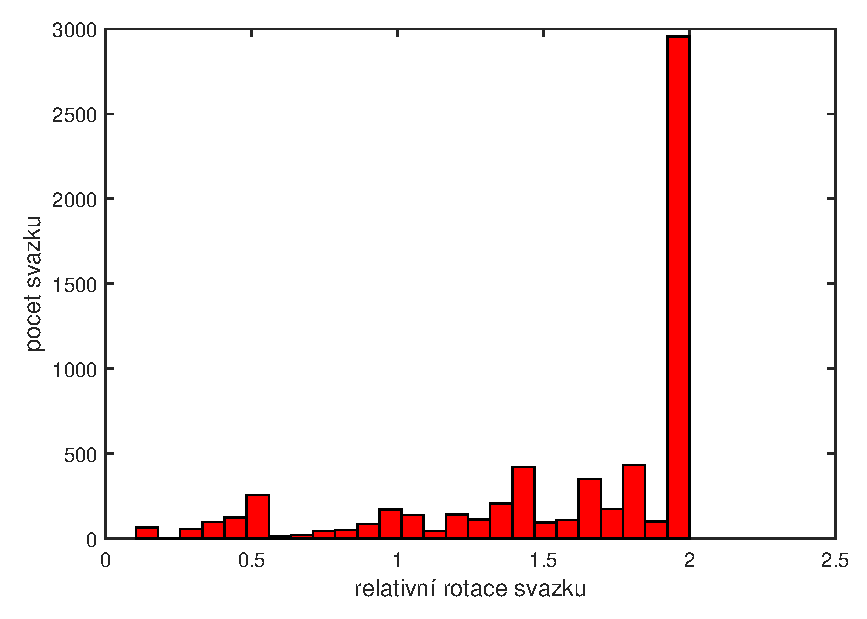
\includegraphics[height =4.5cm]{figures/relative_index1.eps} 
   \end{minipage}
 \end{center}
\caption{Vlevo histogram velikosti natočení světelných svazků kamene VIVA12 z obrázku \ref{fig:relativni pohyb graf}. Vlivem lomu je relativní natočení v mnoha případech vetší než 2. V okolí kritického úhlu roste změna k nekonečnu. Pokud ztotožníme indexy lomu kamene a okolí, tak relativní natočení nebude větší než 2. To lze vidět na histogramu vpravo.}

\label{fig:histogram relativni pohyb }

\end{figure}

Vykresleme si histogram (obr. \ref{fig:histogram relativni pohyb } vlevo) relativní velikosti natočení vystupujících svazků. Z něj je patrné, že řada svazků rotuje o více než dvojnásobek úhlu rotace kamene $\alpha$, což potvrzuje teorii o relativní změně velikosti natočení z rovnice \ref{eq:zmena velikosti posunu}. 



\begin{figure}[h!]
\begin{center}
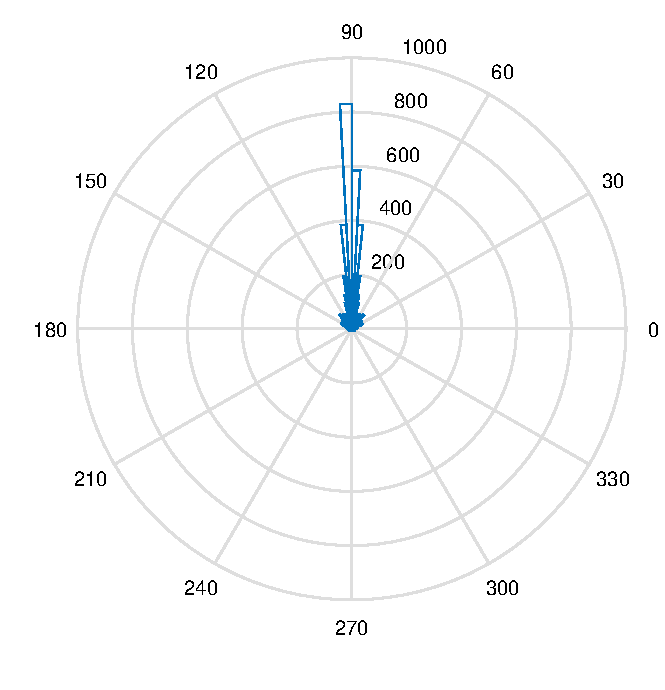
\includegraphics[width = 7cm]{figures/kruhovy_histogram.eps}
\end{center}
\caption{Kruhový histogram směru pohybu jednotlivých světelných svazků kamene VIVA12 z obrázku \ref{fig:relativni pohyb graf}. Většina stop se pohybuje ve směru rotace kamene.}
\label{fig:kruhovy histogram}
\end{figure}

Pokud vezmeme teoreticky kámen o stejném indexu lomu, jako je okolí, neměl by se v kameni lom objevovat. Potom by se velikost rotace výstupního svazku úhel větší než $2\alpha$, způsobená právě rozdílným indexem lomu,  neměla vůbec objevovat. Pro potvrzení této teorie jsme provedli stejnou simulaci jako v předchozím případě. Indexy lomu kamene a jeho okolí jsme ztotožnili a výsledek simulace ukázal, že rotace výstupních svazků úhel větší než $2\alpha$ se již nevyskytují. To nám dokládá zhotovený histogram (obr. \ref{fig:histogram relativni pohyb } vpravo).


\begin{figure}[h!]
\begin{center}
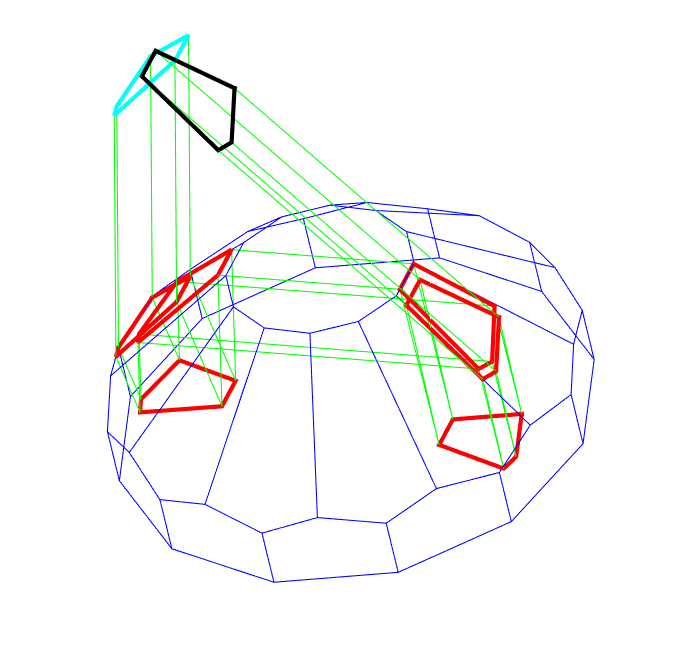
\includegraphics[width = 7cm]{figures/odraz.eps}
\end{center}
\caption{Průlet světelného svazku kamenem VIVA12. Příklad s velkou změnou vystupujícího úhlu. Dopad světelného svazku na fasetu kamene je znázorněn hranolem s modrým okrajem. Svazek vystupující z kamene je hranol s černým okrajem. Svazek kamenem putuje následovně: 1. lom do kamene, 2. odraz od spodku, 3. odraz od fasety, 4. odraz od fasety na protější straně, 5. odraz od spodku, 6. dopad na fasetu pod úhlem blízkým kritickému úhlu a lom z kamene.}

\label{fig:odrazy v kamenu}
\end{figure}
\newpage

Téměř konstantní směrovost rotace svazků u kamene VIVA12 zmenšuje význam příspěvku této vlastnosti k lepšímu rozpoznání světelných stop. Pokud ovšem provedeme stejný experiment na broušeném kameni jiného tvaru, dostaneme rozdílný výsledek. Například u šatonu, svým tvarem složitějším než VIVA12, je směr rotace svazků rozmanitější. Velká část z nich samozřejmě rotuje ve směru rotace kamene. Jak ale vidíme z kruhového histogramu (obr. \ref{fig:kruhovy histogram saton}), lze rozlišovat i velké množství stop pohybujících se např. pod úhlem $45^\circ$. U šatonu tedy může směr pohybu svazků nemalou měrou pomoci v jejich rozpoznání. 

\begin{figure}[h!]
\begin{center}
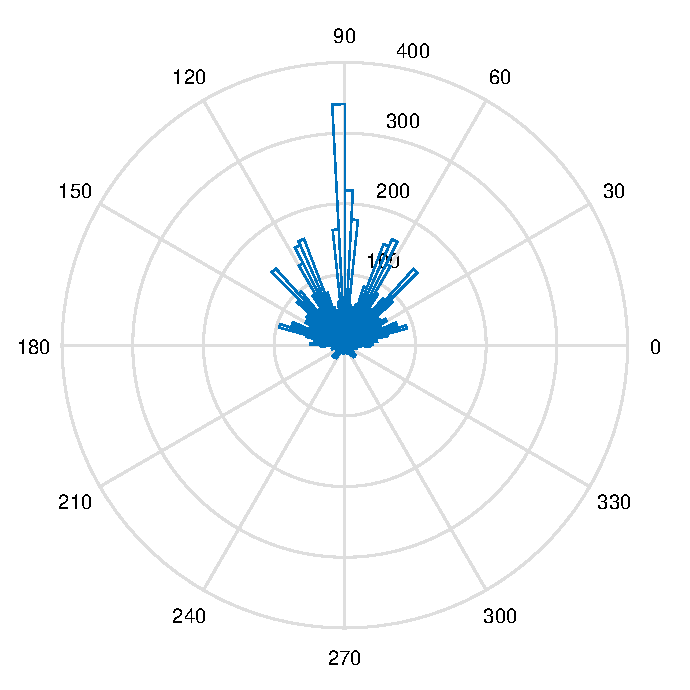
\includegraphics[width = 7cm]{figures/saton_smer.eps}
\end{center}
\caption{Kruhový histogram směru rotace jednotlivých světelných svazků u šatonu. Svazky se natáčí různými směry, kterými lze svazky charakterizovat.}

\label{fig:kruhovy histogram saton}
\end{figure}

  
%\clearpage
\part{Terminologie}

Je důležité rozlišit svazky získané pomocí simulace v LADOKu a svazky získané experimentálním měřením.   
Proto zavedeme \textit{simulované} a \textit{pozorované} svazky.
\vspace{4mm}
\section{Simulované svazky}
\begin{enumerate}

\item 	Získáme potřebné parametry kamene, který zkoumáme. Zdrojem může být technický výkres, nebo předchozí měření.  

\item	Sestavíme model, který bude přibližně určovat tvar kamene. Tento model budeme považovat za \textit{referenční}.

\item	V programu LADOK simulujeme průlet svazku \textit{referenčním} modelem. Pro simulaci je důležité znát polarizaci zdrojového svazku a index lomu kamene. 

\item	Výsledkem simulace jsou parametry \textit{simulovaných} svazků.

\end{enumerate}

\section{Pozorované svazky}
Předpokladem pro získání parametrů pozorovaných svazků je sestavení a kalibrace měřicí soustavy podle \cite{Drapela}. % odkay na kapitolu
\begin{enumerate}

\item 	Opracovaný kámen umístíme do měřicí soustavy.

\item	Provedeme experiment průchodu svazku kamenem podobný situaci v simulačním programu LADOK. 

\item	Získáme obraz dopadu svazků na stínítko. 

\item	V obraze detekujeme světelné stopy (kapitola \ref{sec:detection}).  

\item	Z detekovaných stop vypočítáme parametry \textit{pozorovaných} svazků (kapitola \ref{sec:beam parameters}).

\end{enumerate}

\clearpage
%Přecházíme k situaci, kdy máme dostupné informace o \textit{simulovaných} i \textit{reálných} svazcích. Mezi těmito dvěma množinami je třeba nalézt korespondence. Korespondující svazky si odpovídají seznamem faset kamene, na které při své cestě dopadají.  
%
%Pro korespondující páry určíme chybovou funkci a parametry budeme optimalizovat. Optimalizační algoritmus odhadne takové nastavení parametrů, aby bylo optimalizované kritérium co nejmenší. 
%
%Optimalizované parametry použijeme k výpočtu \textit{optimalizovaného} modelu kamene. Orientace faset broušeného kamene odečteme z \textit{optimalizovaného} modelu.   
\chapter{Optimalizace orientace faset}
	
\section{Postup optimalizace}
	Před tím, než přistoupíme k problému optimalizace, je třeba získat potřebná data. Důležité jsou informace o parametrech svazků, které lze rozdělit na \textit{simulované} a \textit{reálné}.

\subsection*{Simulované svazky}
\begin{enumerate}

\item 	Získáme potřebné parametry kamene, který zkoumáme. Zdrojem může být technický výkres, nebo předchozí měření.  

\item	Sestavíme model, který bude přibližně určovat tvar kamene. Tento model budeme považovat za \textit{referenční}.

\item	V programu LADOK simulujeme průlet svazku \textit{referenčním} modelem. Pro simulaci je důležité znát elektromagnetické vlastnosti laserového svazku a index lomu kamene. 

\item	Výsledkem simulace jsou parametry \textit{simulovaných} svazků.

\end{enumerate}

\subsection*{Reálné svazky}
Předpokladem pro získání parametrů \textit{reálných} svazků je sestavení a kalibrace měřicí soustavy podle \cite{Drapela}. % odkay na kapitolu
\begin{enumerate}

\item 	Opracovaný kámen umístíme do měřicí soustavy.

\item	Provedeme experiment průchodu svazku kamenem podobný situaci v simulačním programu LADOK. 

\item	Získáme obraz dopadu svazků na stínítko. 

\item	V obraze detekujeme světelné stopy (kapitola \ref{sec:detection}).  

\item	Z detekovaných stop vypočítáme parametry \textit{reálných} svazků (kapitola \ref{sec:beam parameters}).

\end{enumerate}

Přecházíme k situaci, kdy máme dostupné informace o \textit{simulovaných} i \textit{reálných} svazcích. Mezi těmito dvěma množinami je třeba nalézt korespondence. Korespondující svazky si odpovídají seznamem faset kamene, na které při své cestě dopadají.  

Pro korespondující páry určíme chybovou funkci a parametry budeme optimalizovat. Optimalizační algoritmus odhadne takové nastavení parametrů, aby bylo optimalizované kritérium co nejmenší. 

Optimalizované parametry použijeme k výpočtu \textit{optimalizovaného} modelu kamene. Orientace faset broušeného kamene odečteme z \textit{optimalizovaného} modelu.   

% diagram je vytvoren -> 500pm -> bitmap -> online to EPS -> latex to PDF -> load PDF
\begin{figure} [h!]
\centering
\includegraphics[width = \textwidth]{diagram.pdf}
\caption{Diagram with princip of cut stone facet orientation estimator.}
\label{fig:diagram}
\end{figure}

\clearpage

\section{Korespondence}

Zdrojový svazek odpadá na maximální možnou plochu kamene. Vlivem toho vystupuje z kamene velké množství svazků. Po dopadu svazků na stínítko je složité zpětně určit, které stopy náleží kterým svazkům.

\subsection{Podmíněnost}
Základní otázkou optimalizačního problému je, zda je systém dostatečně podmíněný. První podmínku, kterou musíme splnit je získat minimálně stejný počet nezávislých rovnic, jako je počet optimalizovaných parametrů. 

V optimalizačním kritériu máme celkem  $2\,r + q$ nezávislých rovnic. Základní podmínkou je, že počet korespondencí musí být minimálně $ s+q $.

To, jak dobře korespondující svazky podmiňují daný model do jisté míry závisí na počtu dopadových faset. Svazky s velkým počtem dopadových faset logicky 



Od tříd \textbf{1A} a \textbf{1B} lze obecně čekat velmi dobrou podmíněnost. Jednotlivý svazek z těchto tříd dopadne pouze na jednu fasetu a směr odraženého svazku jednoznačně určuje parametry fasety, od které se svazek odrazil. Pokud by máš matematický model přesně odpovídal reálnému experimentu, potom postačí nalézt korespondence třídy \textbf{1A} \textbf{1B}, abychom určili parametry všech faset kromě spodku. Tyto třídy nepodmiňují index lomu kamene, pokud bychom chtěli zjistit index
 
 
Teoreticky korespondencí svazků třídy \textbf{3A} (např. UF1-TOP-BOT) získáme 2 rovnice $\Delta e$ a $\Delta \alpha$, které jsou závislé na parametrech dopadových faset UF1, TOP a BOT. Problém spočívá v tom, že tato korespondence určuje pouze vzájemnou polohu dopadových faset a nelze u této třídy očekávat dobrou podmíněnost. 


\subsection{Výpočet odchylek parametrů}

1. možnost - kámen během optimalizace rotujeme. Výsledky rotace si zapamatujeme a odchylky faset budeme počítat vzhledem k parametrů faset rotovaného kamene. 

% je treba popsat, aby se tomu dalo rozumět
2.možnost - Kámen sice rotujeme a optimalizujeme, ale to nic nemění na tom, jak budeme počítat odchylky. Vezmeme si normály faset optimalizovaného a referenčního kamene. Nalezneme rotační matici mezi normálami spodku optimalizovaného a referenčního kamene. Rotační matici aplikujeme i na všechny ostatní fasety. Výsledkem bude to, že kamen srovnáme podle spodku. Chybové parametry pro spodek tak budou nulové.

Dále se postupuje tak, že se nalezne rotace mezi 

\subsection{Pozorování}

Simulujeme průlet světelného svazku optickým klínem (obr. \ref{fig:wedge}). Prostředí s indexy lomu $\eta_1$, $\eta_2$ a $\eta_3$ oddělují rozhraní $\rho_1$ a $\rho_2$. Tyto rozhraní mezi sebou svírají úhel $\alpha$.
\begin{figure}[h!]
\begin{center}
\scalebox{0.8}{ \input{xfig/mirror2.pstex_t}}
\end{center}
\caption{Lom a odraz paprsku v optickém klínu.}
\label{fig:wedge}
\end{figure}

\begin{equation}
\gamma = \arcsin{\left(\frac{\eta_1}{\eta_2}\sin{\beta}\right)}\,.
\end{equation}

\begin{equation}
\varepsilon_1 = \arcsin{\left(\frac{\eta_2}{\eta_1}\sin{\left(\gamma + 2\,\alpha\right)}\right)}\, 
\rightarrow \begin{cases}
\alpha > 0, & \varepsilon_3 > \varepsilon_2 > \varepsilon_1 > \beta\\
\alpha = 0, & \varepsilon_3 = \varepsilon_2 = \varepsilon_1 = \beta\\
\alpha > 0, & \varepsilon_3 < \varepsilon_2 < \varepsilon_1 < \beta
\end{cases}
\end{equation}


Svazek dopadá na rozhraní $\rho_1$ pod úhlem $\beta$. Na obrázku \ref{fig:wedge} je tento svazek reprezentován paprsek č.0. 

Svazek světla můžeme charakterizovat velikostí zářivého toku $\phi_e$. Z Fresnelových rovnic víme, že pokud na rozhraní $\rho_1$ nedochází k totálnímu odrazu, tak po dopadu svazku na rozhraní vznikne odražený a lomený svazek. Jaká bude velikost zářivého toku odraženého svazku $\phi_{e_{reflect}}$ závisí na polarizaci světla, dopadajícím úhlu a poměrem mezi indexy lomu prostředí, které odděluje rozhraní $\rho_1$.

\begin{equation}
\phi_e = \phi_{e_{reflect}} + \phi_{e_{refract}}\,.
\end{equation}

 Při dopadajícím úhlu $\beta = 0^\circ$ a indexech lomu $\eta_1 = 1$, $\eta_2 = 1.5$ se \SI{4}{\percent} dopadajícího zářivého toku odrazí. $\frac{\phi_{e_{reflect}}}{\phi_e} = 0.04$, $\frac{\phi_{e_{refract}}}{\phi_e} = 0.96$.

Z principu šíření světla optickým prostředím pozorujeme svazky 0 až 9, se specifickým směrem šíření. 

V šatonové růži nastává stejný optický jev mezi tabulkou (TOP) a spodkem (BOT), kde
\vspace{4mm}
\begin{tabular}{p{2cm} l}
$\eta_1$ & index lomu vzduchu,\\
$\eta_2$ & index lomu materiálu kamene,\\
$\eta_3$ & index lomu odrazivé vrstvy,\\
$\rho_1$ & tabulka\\
$\rho_2$ & spodek\\
\textbf{0} & zdrojový svazek,\\
\textbf{1} & svazek třídy \textbf{1B} - TOP,\\
\textbf{3} & svazek třídy \textbf{3B} - TOP-BOT-TOP,\\
\textbf{5} & svazek třídy \textbf{5E} - TOP-BOT-TOP-BOT-TOP,\\
\textbf{7} & svazek třídy \textbf{7H} - TOP-BOT-TOP-BOT-TOP-BOT-TOP,\\
\textbf{2,4,6,8} & tyto svazky nevznikají - na rozhraní $\rho_2$ dochází pouze k odrazu.\\
\end{tabular}
\vspace{4mm}

V reálné situaci nejsou fasety TOP a BOT rovnoběžné. Důsledkem toho svazky \textbf{1B}, \textbf{3B}, \textbf{5E} a \textbf{7H} svírají s normálou tabulky různý úhlem. Svazek třídy \textbf{3B} bude mít vždy největší zářivý tok. Zajímavé je, že tyto svazky leží ve stejné rovině. Tato rovina je určena vzájemnou orientací mezi normálou tabulky a normálou spodku.

Po dopadu svazků \textbf{1B}, \textbf{3B}, \textbf{5E} a \textbf{7H} na stínítko můžeme v obraze pozorovat stopy ležící na jedné přímce obr. \ref{fig:wedge_example_image}. 

\begin{figure} [h!]
\centering
\includegraphics[width = 0.9\textwidth]{wedge_example.pdf}
\caption{Zvýraznění obrazů svazků ve snímku. Svazky třídy \textbf{1B}, \textbf{3B}, \textbf{5E} a \textbf{7H} dopadají pouze na fasetu TOP a BOT. Svazky třídy \textbf{3A} a \textbf{5D} dopadnou nejprve na boční fasetu a poté následuje jeden resp. dva dopady na dvojici faset BOT-TOP.}
\label{fig:wedge_example_image}
\end{figure}

 Pokud bychom byli schopni přiřadit alespoň 2 tyto stopy ke svazkům můžeme určit orientaci tabulky a spodku. Situaci ovšem komplikuje fakt, že ne vždy můžeme nalézt obrazy těchto stop, protože jsou zastíněny podstavcem, na který pokládáme kámen. 
 
 U svazků třídy \textbf{3A} a \textbf{5D} dochází k podobnému optickému jevu pouze s tím rozdílem, že svazek do kamene nevstupuje tabulkou, ale boční fasetou. Můžeme si všimnout stejné orientace obrazů dvojice svazků se stejnou vstupující fasetou. Tato dvojice také určuje vzájemnou orientací mezi normálou tabulky a normálou spodku. Pro jednoznačné této orientace je však nutné znát orientaci bočních faset.   

\section{Optimalizované kritérium}
\label{sec:Optimalizace_crit}
Optimalizační algoritmus je převzat z práce \cite{Bodlak2005}. Některé části byly pozměněny. Ukážeme si stručný přehled metody optimalizace a zvýrazníme provedené úpravy. Optimalizační algoritmus používáme nejen k odhadu parametrů faset kamene, ale také k odhadu indexu lomu kamene a jeho orientace kamene v měřené soustavě 

Definujeme kriteriální funkci, kterou budeme optimalizovat. Funkci lze popsat vztahem 

\begin{equation}
\vec{\varepsilon} = h\left(\vec{x},\vec{v},\vec{l},\vec{p} \right)\,,
\end{equation}

\begin{tabular}{l p{12cm}}
$\vec{p}$ & Obsahuje směrové vektory \textit{reálných} svazků. Směr popisujeme pomocí souřadnic azimutu a elevace. Pokud pro výpočet optimalizačního kritéria použijeme $s$ \textit{reálných} svazků, bude mít vektor $\vec{p}$ délku $2\,s$. \\ & \\

$\vec{l}$ & Obsahuje seznam dopadových faset svazku. Tento seznam je využit pro výpočet směru výstupního svazku. Délka seznamu se musí rovnat $s$. \\ & \\

$\vec{v}$ & Popisuje směr zdrojového svazku světla\\ & \\  

$\vec{x}$ & Vektor parametrů, které nastavuje optimalizační algoritmus.
\paragraph{Parametry faset, index lomu}

 Jedná se převážně o parametry $r$ uvolněných faset. Každou fasetu lze parametrizovat pomocí úhlové změny normálového vektoru $\vec{n}$ (2 parametry) a změny vzdálenosti $d$ fasety od souřadného systému (1 parametr).\\
& Optimalizační metoda nemá dostatečnou citlivost na změny vzdálenosti $d$ fasety \cite{Bodlak2005}. Tento parametr proto považujeme za konstantu.\\
& Nově lze mezi optimalizované parametry přidat index lomu kamene $n_i$. Celkově máme $2\,r + q$ parametrů, kde $q$ je 1 pokud je mezi $\vec{x}$ parametr $n_i$, jinak je $q$ rovno 0.

\paragraph{Orientace} Orientaci kamene popisujeme rotací kolem vertikální osy $R_z$ a dvou parametrů definujících náklon kamene $R_x$, $R_y$. 
 \\ & \\

$\vec{\varepsilon}$ & Představuje vektor odchylek v elevaci a azimutu \textit{simulovaných} a \textit{reálných} svazků.\\ 
& V práci \cite{Bodlak2005} byla tato odchylka měřena jako chyba v pozici dopadu laserového svazku na stínítku. Důvodem proč bylo využíváno toto kritérium byla citlivější odezva při změně vektoru svazku. Hlavním důvodem volby azimutu a elevace pro výpočet optimalizačního kritéria je vyšší rychlost. Odpadá totiž potřebný výpočet, který transformuje směrový vektor do souřadnic na stínítku.\\ & Vektor $\vec{\varepsilon}$ má $2\,s$ prvků.\\ & \\

\end{tabular}

\section{Plná vs. zjednodušená simulace}
V optimalizačním cyklu je použito dvou simulací, které simulují průlet světla broušeným kamenem

\subsection{Plná simulace}
Plnou simulací rozumíme klasický program LADOK, který modeluje odraz a lom svazků v konvexním tělese. Nevýhodou algoritmu je ale to, že simulace trvá příliš dlouho na to, aby mohla být úspěšně použita v optimalizačním procesu.

\subsection{Zjednodušená simulace}
Základní myšlenkou je, že se optimalizované parametry $\vec{x}$ příliš nemění. Za tohoto předpokladu si podstatná část svazků zachová posloupnost dopadových faset. Vynecháme proto kontrolu vzniku či zániku svazků. 

Zjednodušená simulace vyřadí z plné simulace zbytečné výpočty, které v procesu optimalizace nevyžíváme. 
Jediné, co potřebujeme znát je směr výstupních svazků. Pro výpočet směru nahradíme svazky nekonečně tenkými paprsky a můžeme s nimi pracovat jako s vektory. Fasety kamene reprezentujeme pomocí normálového vektoru. 

Zjednodušená simulace přistupuje k paprsku jednotlivě. Funkci pro výpočet vektoru výstupního paprsku $\vec{v_o}$ lze vyjádřit jako  

\begin{equation}
\vec{v_o}= g\left(\vec{v_i},\vec{N} \right)\,,
\end{equation}
kde $\vec{v_i}$ je vektor vstupního paprsku. Vektor $\vec{N}$ obsahuje normály $\vec{n_1},\dots,\vec{n_m}$ faset na které svazek dopadá. Normály jsou seřazené v pořadí odpovídající dopadovým fasetám při šíření paprsku od zdroje ke stínítku. 

Při výpočtu musíme vědět, která faseta svazek odráží a která lomí. Situace je jednoduchá. Pokud $m = 1$, potom muselo dojít k odrazu. Pokud  $m > 1$  odpovídají normály $\vec{n_1}$ a $\vec{n_m}$ fasetám, přes které se svazek lomí. Na ostatních fasetách se svazek odrazí. 







Zjednodušená simulace v LAMu pracuje s jinou funkcí. Základním rozdílem je to že navíc počítá polohu, kam paprsek na fasetu dopadl. Výpočet odrazu a jsou v LAMu pomalejší přibližně o \SI{15}{\percent}.

\section{Klasifikace příznaků}



\section{Implementace}
	Uvedeme algoritmy využité pro hledání korespondencí měřených a referenčních svazků a popíšeme jejich aplikaci pro automatické určení náklonu faset broušených kamenů. 
	Předtím, než se začneme zabývat navrženými přístupy, je třeba sjednotit značení jednotlivých parametrů svazků. 
	
	Referenční svazky dělíme do tří množin. 
	
	\begin{tabular}{l l}
	$\mathcal{R}_c$ & - uspořádaná $r_c$-tice svazků, pro které byl nalezen korespondující měřený svazek,\\
	$\mathcal{R}$   & - uspořádaná $r$-tice svazků, ke kterým můžeme přiřadit korespondující měřený savek, \\
	$\mathcal{R}_o$ & - uspořádaná $r_o$-tice svazků, které není možné přidat do množiny korespondencí $\mathcal{C}$.  \\
	\end{tabular}	

Pro tyto množiny platí $\mathcal{R}_c \cap \mathcal{R} = \emptyset$, $\mathcal{R} \cap \mathcal{R}_o = \emptyset$, $\mathcal{R}_c \cap \mathcal{R}_o = \emptyset$, kde $\mathcal{R} = \left(\mathrm{R}_1 ,\,\dots,\, \mathrm{R}_r\right)$. Dále definujeme uspořádanou $r^\prime$-tici $\mathcal{R}^\prime = \mathcal{R} \cup \mathcal{R}_o$. $r^\prime = r +r_o $.
	
	Podobně dělíme měřené svazky na $\mathcal{M}_c$, $\mathcal{M}$, $\mathcal{M}_o$ a $ \mathcal{M}^\prime$, kde $\mathcal{M} = \left(\mathrm{M}_1 ,\,\dots,\, \mathrm{M}_m\right)$.
	 
	 Algoritmy pracují s informacemi o směru, obrazu a zářivém toku $\phi_e$ svazků. Směr vyjadřujeme pomocí azimutu $\alpha$ a elevace $\varepsilon$. Polohu obrazu svazku určuje $x$-ová a $y$-ová souřadnice.
	
	 Parametry referenčních svazků označujeme $\vv{\alpha}_{r}$, $\vv{\varepsilon}_{r}$, $\vv{\phi}_{e_{r}}$, $\vv{x}_r$  a $\vv{y}_r$. Pro měřené svazky platí označení $\vv{\alpha}_{m}$, $\vv{\varepsilon}_{m}$, $\vv{\phi}_{e_{m}}$, $\vv{x}_m$  a $\vv{y}_m$. Platí, že $\vv{\alpha}_{r} = \alpha_{r}\left(\mathcal{R}\right)$, $\vv{\alpha}_{m} = \alpha_{m}\left(\mathcal{M}\right)$ apod. 

Množinu korespondujících svazků značíme $\mathcal{C}$. Jednotlivá korespondence $\mathrm{C}_i$ je uspořádaná dvojice $\left(\mathrm{R}_j,\,\mathrm{M}_k \right)$, $\mathrm{C}_i \subseteq \mathcal{C}$. $\alpha_{r}(\mathrm{C}_i)$ označuje azimut referenčního svazku $\mathrm{R}_j$, kde $\mathrm{R}_j \subset \mathrm{C}_i$ a $\alpha_{r}(\mathcal{C})$ vektor $\left(\alpha_{r}(\mathrm{C}_1),\,\dots,\,\alpha_{r}(\mathrm{C}_n)\right)$, kde $n$ je počet uspořádaných dvojic v množině $\mathcal{C}$.
	
	 

\subsection{Použité algoritmy}
	Korespondence hledáme buď pro specifickou třídu třídu svazků nebo pro svazky, které splní požadované parametry. 

\subsubsection{Korespondence svazků třídy \textbf{1A}}
\label{sec: 1A}

Víme, že svazky třídy \textbf{1A} se odráží od faset \textbf{UF1} - \textbf{UF2}. Úhlová odchylka normály referenční fasety skutečné normály se projeví dvojnásobnou úhlovou odchylkou referenčního svazku od měřeného. Očekáváme, že rozdíl mezi referenčními a reálnými parametry faset není příliš velký. Proto lze očekávat, že měřené svazky třídy \textbf{1A} budou mít velmi podobný směr jako referenční. Přibližně tedy známe směr těchto svazků.

V blízkém okolí stop třídy \textbf{1A} se mohou nacházet pouze stopy s řádově nižším zářivým tokem. Tato vlastnost je zajištěna geometrií kamene \textit{viva12} a provedením experimentu. Pokud známe zářivý tok stop, můžeme v obraze snadno nalézt svazek třídy \textbf{1A}. 

\paragraph{Parametry algoritmu}
\hspace{1mm}
	 
	 \begin{tabular}{l l}
	 $d_{max}$ & - kvadrát maximální vzdálenosti měřeného svazku od referenčního,\\
	 $n_{min}$ & - minimální počet měřených svazků, v blízkém okolí referenčního svazku, s nižším zářivým tokem než zářivý tok potenciálního korespondujícího měřeného svazku. \\
	 \end{tabular}
	
\paragraph{Popis algoritmu} 

\begin{enumerate}
\item Definujeme proměnné $\alpha_{c} = 0$, $\varepsilon_{c} = 0$, $\mathcal{C} = \emptyset$, $\mathcal{C}_{l} = \emptyset$.

\item $i = 0$.

\item Vypočítáme kritérium hodnotící vzdálenost mezi svazky 

$\vv{d} = (\alpha_{r}(\mathrm{R}_i)\cdot\vv{\mathbf{1}}-\vv{\alpha}_{m}-\alpha_{c}\cdot\vv{\mathbf{1}})^2 + (\varepsilon_{r}(\mathrm{R}_i)\cdot\vv{\mathbf{1}}-\vv{\varepsilon}_{m}-\varepsilon_{c}\cdot\vv{\mathbf{1}})^2 $.

\item Vybereme uspořádanou $k$-tici svazků $\mathcal{N}$ z $\mathcal{M}$, která odpovídá rostoucí posloupnosti $\vv{d}$ a omezení na $\vv{d} < d_{max}$. $\mathcal{N}_1 \sim \argmin(d)\,$ tak, že $\mathcal{N} = \left(\mathrm{M}_a ,\,\dots,\, \mathrm{M}_b \right)$, kde $a = \argmin(\vv{d})$ a $b = \argmin\left(\dfrac{1}{\vv{d}-d_{max}}\right)$. Dále bude platit, že  $\mathrm{N}_1 = \mathrm{M}_a$ a $\mathrm{N}_k = \mathrm{M}_b$ apod. 

\item Nalezneme uspořádanou $k$-tici $\mathcal{O}$ takovou, že $\mathcal{O} = \left(\mathrm{N}_1 ,\,\mathrm{N}_e,\,\mathrm{N}_f ,\,\dots,\, \mathrm{N}_g \right)$, kde\\$e = \argmin\left( \phi_{e_{m}}\left(\mathrm{N}_1 \right),\, \phi_{e_{m}}\left(\mathrm{N}_2 \right)  \right)$, $f = \argmin\left( \phi_{e_{m}}\left(\mathrm{N}_1 \right),\, \phi_{e_{m}}\left(\mathrm{N}_2 \right),\, \phi_{e_{m}}\left(\mathrm{N}_3 \right)   \right)$ a \\  $g = \argmin\left( \phi_{e_{m}}\left(\mathrm{N}_1 \right),\,\dots,\, \phi_{e_{m}}\left(\mathrm{N}_k \right)  \right)$.  

\item Určíme vektor $\vv{n_\mathcal{O}}$ o velikosti $k$ udávající četnost prvků z množiny $\mathcal{N}$ v množině $\mathrm{O}$. Pokud $\mathrm{O}_q = \mathcal{O}_s$, tak $n_{\mathcal{O}}(q) = n_{\mathrm{O}}(s)$, pro $q = \lbrace1,\,\dots,\,k \rbrace$ a podobně $s = \lbrace 1,\,\dots,\,k \rbrace$.

\item Určíme minimální $l$, které splňuje alespoň jednu z podmínek $n_{\mathcal{O}}(l) > n_{min}$  a $l = k$. Do množiny $\mathcal{C}$ přidáme korespondenci $\left(\mathrm{R}_i,\,\mathrm{N}_l \right)$.

\item Pokud $i \neq r$, tak $i = i+1$ a opakujeme body 3) až 7).

\item Pokud $\mathcal{C}_{l} \neq \mathcal{C}$, vypočítáme korekční parametry $\alpha_{c} = median(\alpha_{r}(\mathcal{C})-\alpha_{m}(\mathcal{C}))$, \\ $\varepsilon_{c} = median(\varepsilon_{r}(\mathcal{C})-\varepsilon_{m}(\mathcal{C}))$, položíme $\mathcal{C}_{l}$ rovno $\mathcal{C}$  a opakujeme body 2) až 8).

\item Z $\mathcal{C}$ odstraníme prvky, ve kterých se obraz referenčního svazku nachází mimo obraz stínítka.

\item Optimalizujeme náklon kamene (kapitola \ref{sec:Optimalizace_crit}).

\item Podle výsledku optimalizace upravíme model kamene a přepočítáme parametry referenčních svazků. Opakujeme bod 1) až 10). V příští iteraci tento bod vynecháme. 

\item Z $\mathcal{C}$ odstraníme prvky, ve kterých se obraz referenčního svazku nachází mimo obraz stínítka.

\end{enumerate}
\newpage
\subsubsection{Korespondence svazků třídy \textbf{3A}}	
\label{sec:3A}
	Po optimalizaci podle třídy \textbf{1A} máme dobře odhadnuté parametry faset \textbf{UF1} - \textbf{UF12}. Pomocí rotace a náklonu kamene odhadneme přibližně parametry faset \textbf{TOP} a \textbf{BOT}. Podstatné je, že svazek třídy \textbf{3A} dopadá na tabulku \textbf{TOP} pod výrazně menším úhlem, než je kritický úhel. To zajišťuje přijatelnou citlivost směru svazků na změnu parametrů dopadových faset. 
	
	Referenční svazky třídy \textbf{3A} mají po třídě \textbf{3B} druhý nejvyšší zářivý tok. Ostatní třídy se vyznačují řádově nižším zářivým tokem. Podle zářivého toku $\phi_{e_r}$  lze tedy snadno oddělit svazky se třemi dopadovými fasetami od ostatních svazků. Referenčních svazků třídy \textbf{3A} a \textbf{3B} je celkem 13. Často nastává situace, že svazek třídy \textbf{3B} nedetekujeme, protože je jeho obraz zakrytý podstavcem na kámen. 
	
	Separaci podle zářivého toku  však nelze s jistotou použít u měřených svazků. Pokud dojde k překrytí obrazu svazků jiných tříd, může být zářivý tok tohoto shluku větší. Spolehlivý způsob, jak oddělit měřené svazky třídy \textbf{3A} a \textbf{3B} od ostatních, je porovnat maximální úrovně jasu v obrazech svazků.  
	
	Další vlastnost, která dobře charakterizuje svazky třídy \textbf{3A} jsou dlouhé a intenzivní ocásky. Při hledání korespondencí můžeme využít párování svazků podle charakteru ocásků (kapitola \ref{sec: korespondence_ocasky}). Výhodou algoritmu je to, že dokážeme za vhodného nastavení nalézt korespondující svazky, a to i v případě vysokých směrových odchylek svazků. Nevýhodou je necitlivost na ostatní parametry svazků. 

\paragraph{Popis algoritmu} 

\begin{enumerate}
	\item Redukujeme počet měřených svazků a vytvoříme uspořádanou 13-tici $\mathcal{M}$ obsahující prvních 13 měřených svazků s nejvyšší hodnotou jasu v obraze. 

	\item Podle podobnosti ocásků nalezneme počáteční odhad množiny korespondencí $\mathcal{C}$ (kapitola \ref{sec: korespondence_ocasky})). Parametry algoritmu: $\sigma = 0.2$, $L_{min} = 2$, $\Delta\alpha_{max} = 35^\circ$, $\Delta\varepsilon_{max} = 15^\circ$.
	
	\item Uvolníme pouze parametry faset \textbf{TOP} a \textbf{BOT}. V tomto kroku prohlásíme parametry těchto dvou faset za totožné a optimalizujeme parametry uvolněných faset (kapitola \ref{sec:Optimalizace_crit}). Pokud neznáme dostatečně přesně index lomu kamene optimalizujeme také index lomu. 
	
	\item Podle výsledku optimalizace upravíme model kamene a přepočítáme parametry referenčních svazků. Pro finální odhad množiny korespondencí $\mathcal{C}$ použijeme algoritmus v kapitole \ref{sec: 1A} od bodu 1) do bodu 10). $\mathcal{R}$ bude uspořádaná 24-tice referenčních svazků třídy \textbf{1A} a \textbf{3A}. $\mathcal{M}$ bude obsahovat všechny měřené svazky.  
	
	\item K optimalizovaným parametrům přidáme parametry faset \textbf{UF1} až \textbf{UF12} a optimalizujeme. 
		
\end{enumerate}

\newpage
\subsubsection{Korespondence svazků třídy \textbf{5D}}
\label{sec:5D}
	Svazky třídy \textbf{5D} můžeme v obraze pozorovat, pokud existuje úhlová odchylka mezi fasetou \textbf{TOP} a \textbf{BOT}. Předpokládáme, že pokud nějaká odchylka vznikne, bude max. \SI{1}{\degree}. Také předkládáme, že normály faset \textbf{UF1} až \textbf{UF12} nejsou vůči pravidelnému tvaru \textit{vivy12} příliš vychýleny.
	
	Podstatné je, že známe polohu svazků třídy \textbf{3A}. Za výše uvedených okolností lze pozorovat vzor určující vzájemnou polohu dvojice svazků třídy \textbf{3A} a \textbf{5D}, které mají v seznamu stejné dopadové fasety např. dvojice (UF1-TOP-BOT, UF1-TOP-BOT-TOP-BOT). Vzájemnou polohu mezi všemi těmito páry lze popsat pomocí polárních souřadnic vzdáleností $\rho$ a úhlem $\varphi$. 
	
	Polohu j-tého měřeného svazku popisujeme souřadnicemi $x_m(\mathrm{M}_j)$ a $y_m(\mathrm{M}_j)$. Měřené svazky rozdělíme na uspořádanou $n$-tici $\mathcal{N}$ obsahující 12 svazků třídy 3A a uspořádanou $o$-tici $\mathcal{O}$ obsahující zbylé svazky. 

\paragraph{Parametry algoritmu}
\hspace{1mm}

	 \begin{tabular}{l l}
	 $\rho_{max}$ & - maximální vzdálenost obrazu svazků třídy \textbf{3A} a \textbf{5D} v pixelech,\\
	 $\Delta\rho$ & - maximální absolutní odchylka úhlu v obraze mezi párem svazků třídy \textbf{3A} a \textbf{5D},\\
	 $\Delta\varphi$ & - maximální absolutní odchylka vzdálenosti v obraze mezi párem svazků třídy \textbf{3A} a \textbf{5D},\\
	 $p_{min}$ & - minimální počet nalezených dvojic.\\
	 \end{tabular}

\paragraph{Algoritmus}

\begin{enumerate}
\item Vypočítáme Euklidovu vzdálenost obrazů jednotlivých svazků

$\rho_{j,k} = \sqrt{\left( x_m(\mathrm{N}_j) - x_m(\mathrm{O}_k) \right)^2 + \left( y_m(\mathrm{N}_j) - y_m(\mathrm{O}_k) \right)^2}$ 

pro $j = \lbrace 1,\,\dots,\,n \rbrace$ a $k = \lbrace 1,\,\dots,\,o \rbrace$. 

Směrový úhel určíme podle vztahu $\varphi_{j,k} = \arctan\dfrac{y_m(\mathrm{N}_j) - y_m(\mathrm{O}_k)}{x_m(\mathrm{N}_j) - x_m(\mathrm{O}_k)}$.

\item Vybereme svazky vzdálené méně než $\rho_{max}$ a dostaneme vektor vzdáleností $\vv{\rho}$ a směrových úhlu $\vv{\varphi}$.

$\lbrace \varphi_{j,k} \subseteq \vv{\varphi},\,\rho_{j,k} \subseteq \vv{\rho}\,|\,\, \rho_{j,k} < \rho_{max} \rbrace$ pro $j = \lbrace 1,\,\dots,\,n \rbrace$ a $k = \lbrace 1,\,\dots,\,o \rbrace$,
 
 kde  $\vv{\varphi} = (\varphi_{{j_1},{k_1}},\,\dots,\,\varphi_{{j_s},{k_s}}) = (\varphi_{1},\,\dots,\,\varphi_{s})$ a $\vv{\rho} = (\rho_{{j_1},{k_1}},\,\dots,\,\rho_{{j_s},{k_s}}) = (\rho_{1},\,\dots,\,\rho_{s})$. 

\item Definujeme funkce $g(x)\rightarrow \begin{cases}
1, & |x| < \Delta\rho\\
0, & jinak
\end{cases}\,, \hspace{4mm}h(x) \rightarrow \begin{cases}
1, & |x| < \Delta\varphi\\
0, & jinak
\end{cases}$. 

Pro vektor $\vv{x}$ délky $n$ platí $g(\vv{x}) = \left(g(x_1),\,\dots,\,g(x_n)\right)$ a $h(\vv{x}) = \left(h(x_1),\,\dots,\,h(x_n)\right)$.

 Nechť $a = \underset{{q = \lbrace1,\,\dots,\,s\rbrace}}{\argmax}\,\, \overset{s}{\underset{{i = 1}}{\sum}} g\left(\varphi_i-\varphi_q\right)$, \hspace{4mm} $b = \underset{{q = \lbrace1,\,\dots,\,s\rbrace}}{\argmax}\,\, \overset{s}{\underset{{i = 1}}{\sum}} h\left(\rho_i-\rho_q\right)$, potom 

$\vv{\upsilon} = g\left(\vv{\varphi} - \varphi_a\cdot\vv{\mathbf{1}} \right) + h\left(\vv{\rho} - \rho_b\cdot\vv{\mathbf{1}} \right)$.


\item Nalezeme množinu potenciálních korespondencí $\mathcal{C^\prime}$. $\lbrace \left(\mathrm{R}_t,\mathrm{O}_{k_q}\right) \subseteq \mathcal{C^\prime} \,|\,\, \upsilon_q > 1 \rbrace$, pro $q = \lbrace1,\,\dots,\,s\rbrace$, kde $R_t$ je referenční svazek třídy \textbf{5D} se stejným seznamem dopadajících faset jako měřený svazek $\mathrm{N}_{j_q}$.

\item Pokud $\mathcal{C^\prime}$ obsahuje alespoň $p_{min}$ prvků, přidáme $\mathcal{C^\prime}$ do množiny korespondencí $\mathcal{C}$.

 
\end{enumerate}

\newpage
\subsubsection{Korespondence svazků podle polohy v obraze a zářivého toku}
	Tento algoritmus se snaží o to nalézt dvojici svazků, které se promítnou na podobnou pozici v obraze a mají vysoký zářivý tok. Snažili jsme se nalézt funkci, která by charakterizovala závislost mezi zářivým tokem $\phi_{e_{r}}$ referenčních stop a zářivým tokem $\phi_{e_{m}}$ měřených stop. Jednoduchou funkci jsme však nenašli. Ke korespondenci svazků budeme místo absolutního zářivého toku využívat jeho relativní velikosti vzhledem k ostatním svazkům v blízkém okolí. 

\paragraph{Parametry algoritmu}
\hspace{1mm}

	 \begin{tabular}{l l}
	 $\rho_{max}$ & - maximální vzdálenost obrazu svazků třídy \textbf{3A} a \textbf{5D} v pixelech,\\
	 $\Delta\rho$ & - maximální absolutní odchylka úhlu v obraze mezi párem svazků třídy \textbf{3A} a \textbf{5D},\\
	 $\Delta\varphi$ & - maximální absolutní odchylka vzdálenosti v obraze mezi párem svazků třídy \textbf{3A} a \textbf{5D},\\
	 $p_{min}$ & - minimální počet nalezených dvojic.\\
	 \end{tabular}

\paragraph{Algoritmus}

\begin{enumerate}
\item $j = 1$, $\vv{w}_{m^\prime} = \vv{\mathbf{1}}$, $\vv{w}_{r^\prime} = \vv{\mathbf{1}}$. 

\item Nalezneme 3 svazky $\left(\mathrm{M}^\prime_a,\,\mathrm{M}^\prime_b,\,\mathrm{M}^\prime_c \right) \subset \lbrace \mathcal{M}^\prime\setminus \mathrm{M}^\prime_j\rbrace$ s nejmenší Euklidovou vzdáleností obrazu $\left(d_a,\,d_b,\,d_c\right)$ od svazku $\mathrm{M}^\prime_j$.

$d_a = \sqrt{\left( x_{m}(\mathrm{M}_j^\prime) -  x_{m}(\mathrm{M}_a^\prime) \right)^2 + \left( y_{m}(\mathrm{M}_j^\prime) -  y_{m}(\mathrm{M}_a^\prime) \right)^2}$.

\item Nechť $f(\mathrm{M}^\prime_x)\rightarrow \begin{cases}
\phi_{e_{m}}\left(\mathrm{M}^\prime_x \right), & d_x < d_{m_{max}}\\
1, & jinak
\end{cases}$, $\phi_{e_{m}}(\mathrm{M}^\prime_j) > 1 $ potom 

$\phi_{m^\prime_{max}} = \max\left(\phi_{e_{m}}(\mathrm{M}^\prime_j),\,f(\mathrm{M}^\prime_a),\,f(\mathrm{M}^\prime_b),\,f(\mathrm{M}^\prime_c)  \right)$. 

\item Nastavíme váhy měřených svazků.

 $w_{m^\prime_{q}} = \dfrac{\phi_{max}}{f(\mathrm{M}^\prime_q)}$ pro $q = \lbrace j,\,a,\,b,\,c \rbrace$.
 
\item Nalezneme uspořádanou $s$-tici $\mathcal{S} = (\mathrm{S}_1,\,\dots,\,\mathrm{S}_s)$ referenčních svazků z $\mathcal{R}^\prime$. 

$\lbrace \mathrm{R}^\prime_i \subseteq \mathcal{S}\,|\,\, d_{i,j} < d_{r_{max}}  \rbrace$ pro $i = \lbrace 1,\,\dots,\, r^\prime \rbrace$, kde 

$d_{i,j} = \sqrt{\left( x_{m}(\mathrm{M}_j^\prime) -  x_{r}(\mathrm{R}_i^\prime) \right)^2 + \left( y_{m}(\mathrm{M}_j^\prime) -  y_{r}(\mathrm{R}_i^\prime) \right)^2}$.

\item $w_{r^\prime_j} = max\left( \phi_{e_r}(\mathcal{S}) \right)$.

\item Dokud $j \neq n^\prime$, $j = j+1$ a opakujme body 2) až 6). 

\item Nechť  $g(x)\rightarrow \begin{cases}
x, & x > 1\\
1, & jinak
\end{cases}$, potom můžeme určit kriteriální funkci 

$\mathbf{L}(i,j) = d_{i,j}\cdot w_{m^\prime_{j}} \cdot g \left(\dfrac{\phi_{r_i}(\mathcal{R}^\prime_i)}{w_{r^\prime_{j}}} \right)$. 


\item Potenciální korespondence $\mathcal{C}^\prime$ nalezneme podle vzájemně nejnižší velikosti  kritéria v $\mathbf{L}$, které nepřekročí hodnotu $L_{max}$. Korespondující dvojice $\left(\mathrm{R}^\prime_i,\,\mathrm{M}^\prime_j \right) \subseteq \mathcal{C}^\prime$, pokud\\ $i = \underset{{q = \lbrace1,\,\dots,\,r^\prime\rbrace}}{\argmin}\mathbf{L}(q,j)$, $j = \underset{{q = \lbrace1,\,\dots,\,m^\prime\rbrace}}{\argmin}\mathbf{L}(i,g)$ a  $\mathbf{L}(i,j) < L_{max}$. 

\item Vybereme korespondence z $\mathcal{C}^\prime$, které můžeme přidat do množiny korespondencí $\mathcal{C}$. 

 $\lbrace \mathrm{C}^\prime_l \in \mathcal{C}\,|\,\, \mathrm{C}^\prime_l \subseteq \lbrace\mathcal{R}_f \cup \mathcal{M}_f\rbrace \rbrace$.

 
\end{enumerate}

\newpage
\subsubsection{Korespondence svazků podle ocásků}
\label{sec: korespondence_ocasky}
		
	Ocásky svazků definujeme pomocí velikosti a směrového úhlu.
	
	Počet ocásků referenčního svazku závisí na počtu stran polygonu, kterým popisujeme tvar svazku. Intenzitu ocásku v simulaci určuje zářivý tok svazku a na velikost hrany, na které ocásek vzniká. 
	
	Velikost $\vv{\xi}_{r}\left(\mathrm{R_i}\right)$ a směrový úhel $\vv{\psi}_{r}\left(\mathrm{R_i}\right)$ ocásků  $i$-tého referenčního svazku $\mathrm{R_i}$ určuje vektor o délce $n_i$.\\
	 $\vv{\xi}_{r}\left(\mathrm{R_i}\right) = \left(\xi_{r_1}\left(\mathrm{R_i}\right),\,\dots,\,\xi_{r_{n_i}}\left(\mathrm{R_i}\right)\right)$, $\vv{\psi}_{r}\left(\mathrm{R_i}\right) = \left(\psi_{r_1}\left(\mathrm{R_i}\right),\,\dots,\,\psi_{r_{n_i}}\left(\mathrm{R_i}\right)\right)$, kde $n_i$ je počet ocásků $\mathrm{R_i}$. 
	
	Detekce ocásků měřeného svazku je popsána v kapitole \ref{sec:tails}. Obecně platí, že v obraze jsou detekovatelné ocásky, pro které byla v odpovídající simulaci vypočítána vysoká intenzita. 
	
	Velikost ocásků $j$-té měřené stopy značíme $\vv{\rho}_{m}\left(\mathrm{M_j}\right)$, směrový úhel $\vv{\varphi}_{m}\left(\mathrm{M_j}\right)$. 
	 
	 Podobnost ocásků hodnotíme podle kritéria, a to především na základě podobnosti směru ocásků. Velikost ocásků určuje váhu jednotlivých příspěvků.
	 
\paragraph{Parametry algoritmu}
\hspace{1mm}
	 
	 \begin{tabular}{l l}
	 $\Delta\alpha_{max}$ & - maximální absolutní odchylka azimutu měřeného svazku od referenčního,\\
	 $\Delta\varepsilon_{max}$ & - maximální absolutní odchylka elevace měřeného svazku od referenčního,\\
	 $\sigma$ & - citlivost kriteriální funkce na úhlovou odchylku ocásků,\\
	 $L_{min}$ &  - minimální velikost kritéria  $\mathbf{L} \in \mathbb{R}^{r\times m}$ pro přidání dvojice svazků do množiny korespondencí $\mathcal{C}$. \\
	 \end{tabular}
	
\paragraph{Algoritmus}

\begin{enumerate}
\item $i = 1$

\item Normujeme velikost referenčních ocásků $\vv{\xi}_r\left( \mathrm{R_i} \right) = \dfrac{\vv{\xi}_r\left( \mathrm{R_i} \right)}{\max \left( \vv{\xi}_r\left( \mathrm{R_i} \right) \right)}\,.$

\item Z referenčních ocásků vybereme pouze ty s dominantní intenzitou a získáme vektor velikost $\vv{\rho}_{r}\left(\mathrm{R_i}\right)$ a směr $\vv{\varphi}_{r}\left(\mathrm{R_i}\right)$ o délce $n_k$.\\ $\lbrace \psi_{r_k}\left(\mathrm{R_i}\right) \subseteq \vv{\varphi}_{r}\left(\mathrm{R_i}\right),\, \xi_{r_k}\left(\mathrm{R_i}\right) \subseteq \vv{\rho}_{r}\left(\mathrm{R_i}\right)\,|\,\, \xi_{r_k}\left(\mathrm{R_i}\right) > \xi_{min} \rbrace$, kde $k =\lbrace 1,\,\dots,\,n_i\rbrace $.

\item Nalezneme uspořádanou $n$-tici $\mathcal{N}$ z měřených svazků $\mathcal{M}$. \\$\lbrace \mathrm{M}_j \subseteq \mathcal{N} \,\,|\,\,|\alpha_r(\mathrm{R}_i) - \alpha_m(\mathrm{M}_j) | < \Delta\alpha_{max},\, |\varepsilon_r(\mathrm{R}_i) - \varepsilon_m(\mathrm{M}_j) | < \Delta\varepsilon_{max} \rbrace$, kde $j =\lbrace 1,\,\dots,\,m \rbrace $.


\item Pokud $ \mathrm{M}_j \subseteq \mathcal{N}$, \\
  $\mathbf{L}(i,\,j) = \overset{n_k}{\underset{{k = 1}}{\sum}}\, \overset{n_l}{\underset{{l = 1}}{\sum}}\,\dfrac{1}{\sqrt{2\pi}\, \sigma}\cdot e^{-\dfrac{\left(\varphi_{r_k}(\mathrm{R}_i)- \varphi_{m_l}(\mathrm{M}_j) \right)^2}{2\sigma^2}} \cdot \sqrt{\rho_{r_k}(\mathrm{R}_i)\, \rho_{m_l}(\mathrm{M}_j)}\,,$
  \\jinak $\mathbf{L}(i,j) = 0$, pro $j =\lbrace 1,\,\dots,\,m \rbrace $, kde $n_l$ je počet ocásků $\mathrm{M_j}$.
  

\item Pokud $i \neq r$, $i = i+1$ a opakujeme kroky 2) až 5).

\item Korespondující svazky nalezneme podle vzájemně nejvyššího kritéria v $\mathbf{L}$ s minimální velikostí $L_{min}$. Korespondující dvojice $\left(\mathrm{R}_i,\,\mathrm{M}_j \right) \subseteq \mathcal{C}$, pokud  $i = \underset{{q = \lbrace1,\,\dots,\,r\rbrace}}{\argmax}\mathbf{L}(q,j)$,\\ $j = \underset{{q = \lbrace1,\,\dots,\,m\rbrace}}{\argmax}\mathbf{L}(i,g)$ a  $\mathbf{L}(i,j) > L_{min}$. 

\end{enumerate}

\newpage
\subsection{Automatická optimalizace}
Kámen je do měřicí soustavy umístěn ručně tak, aby se vertikální osa kamene nacházela v těžišti dopadajícího zdrojového svazku. Kamen je položen na spodku a laserový svazek dopadá na tabulku a boční fasety. Takto je zajištěna poloha kamene, ovšem rotace kamene okolo vertikální osy může být libovolná a musí být nalezena před optimalizací parametrů faset kamene. 

Podle plochy, na kterou pokládáme kámen nemůžeme automaticky určit orientaci fasety BOT. Podstavec není pevně přichycen a mezi fasetou BOT a podstavcem je navíc reflexní vrstva. Pokud není reflexní vrstva nanesena rovnoměrně je kámen v měřicí soustavě nakloněn.

Náklon kamene určíme při hledání korespondencí svazků třídy \textbf{1A}. 




\section{Výsledky}

\subsection{}

















 \clearpage
\part{Korespondence svazků}

Kámen vložený do měřicí soustavy vytvoří na stínítku specifický obrazec. Pokud vytvoříme vhodný matematický model této situace a aplikujeme na něj optické zákony, dostaneme stejný obrazec. 

Úloha optimalizace náklonu faset spočívá v nalezení korespondujících svazků. Korespondence je uspořádaná dvojice měřeného a referenčního svazku. Korespondující svazky mají společnou posloupnost dopadových faset. 

\section{Složitost úlohy}
	Korespondence nelze nalézt všechny najednou. Ve snímku \ref{fig: kores_faze_0} jsou zobrazeny vzdálenosti korespondujících svazků po optimalizaci náklonu a rotace kamene. Vzdálenost většiny korespondujících svazků je příliš vysoká na to, abychom mohli korespondence nalézt. Situace je navíc komplikována tím, že řada referenčních svazků, kterým v odraze odpovídá měřený svazek neexistuje. Ve fázi optimalizace na obrázku \ref{fig: kores_faze_0} neexistuje \SI{36}{\percent} referenčních svazků, k nimž později přiřadíme korespondující měřený svazek. 
	
	  V prvním kroku lze nalézt korespondence pouze pro vybrané třídy svazků. Jedná se o třídy \textbf{1A}, \textbf{3A} a ne vždy detekované třídy \textbf{3B} a \textbf{5D} viz obr. \ref{fig:wedge_example_image}. 
	
	Čekali bychom, že pokud optimalizujeme náklon faset s korespondencemi svazků, které lze určit v počátku, budou obrazy ostatních korespondujících svazků téměř totožné. Na obr. \ref{fig: kores_faze_1} ovšem vidíme, že ani v tomto případě nelze určit všechny korespondence. Vzdálenosti obrazů korespondujících svazků stále znatelné. Zvláště pak máme problém nalézt korespondence v oblastech s vysokou hustotou svazků. Je zřejmé, že korespondence budeme muset nacházet ve více krocích a postupně parametry faset přibližovat ke konečnému výsledku náklonu. 

Indikátorem, zda jsme nastavili správně parametry faset kamene, je vzdálenost měřených a referenčních svazků. Po optimalizaci náklonu faset podle korespondujících svazků (obr. \ref{fig: kores_faze_2}) vidíme, že směry korespondujících svazků v mnoha případech nesouhlasí. Navíc můžeme pozorovat měřené svazky, ke kterým neexistuje vhodný referenční svazek a naopak vidíme také volné referenční svazky. Na tyto nepřesnosti má vliv zakřivení faset, neurčitost vzdálenosti faset, nepřesná kalibrace, detekce atd.  

 
 \begin{figure}[htbp]
    \centering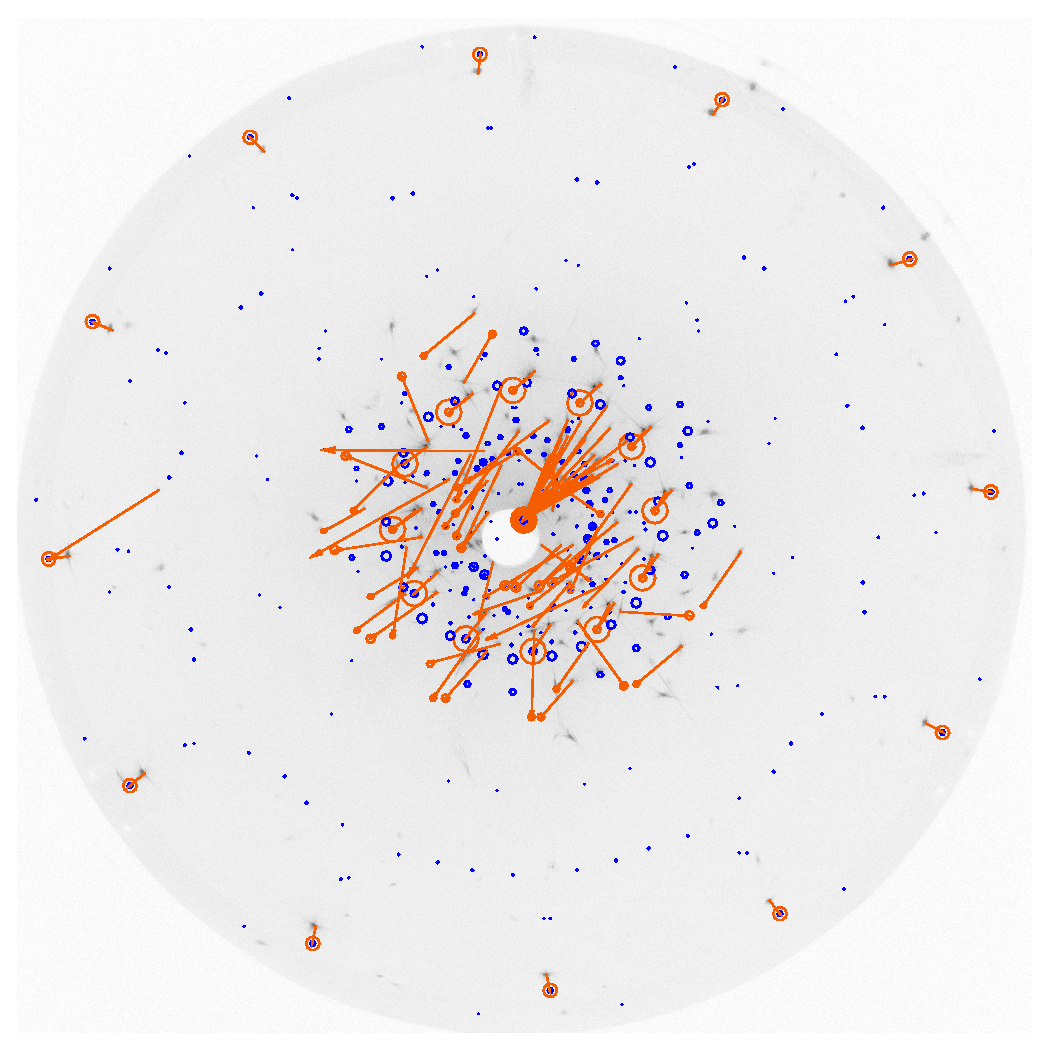
\includegraphics[width=\textwidth]{kores_faze_1.eps}
    \caption[Vzdálenost korespondujících svazků - fáze 0.]{Vzdálenost korespondujících svazků po optimalizaci náklonu a rotace kamene \textit{viva12}. Kružnice znázorňují referenční svazky. Čím vyšší je zářivý tok svazku, tím vyšší je poloměr kružnice. Vektory směřují od obrazu měřeného svazku k obrazu korespondujícího referenčního svazku. Modrou barvou jsou zobrazeny referenční svazky, pro které nebyl nalezen korespondující měřený svazek.}
 \label{fig: kores_faze_0}
 \end{figure}

 
 \begin{figure}[htbp]
    \centering\includegraphics[width=\textwidth]{kores_faze_3.eps}
    \caption[Vzdálenost korespondujících svazků - fáze 1.]{Vzdálenost korespondujících svazků po optimalizaci náklonu faset podle korespondencí, které lze spolehlivě nalézt. Kružnice znázorňují referenční svazky. Čím vyšší je zářivý tok svazku, tím vyšší je poloměr kružnice. Vektory směřují od obrazu měřeného svazku k obrazu korespondujícího referenčního svazku. Zelenou barvou jsou zobrazeny korespondence použité při optimalizaci parametrů kamene. Modrou barvou jsou zobrazeny referenční svazky, pro které nebyl nalezen korespondující měřený svazek. Detail na střední část snímku.}
 \label{fig: kores_faze_1}
 \end{figure}
 
  \begin{figure}[htbp]
    \centering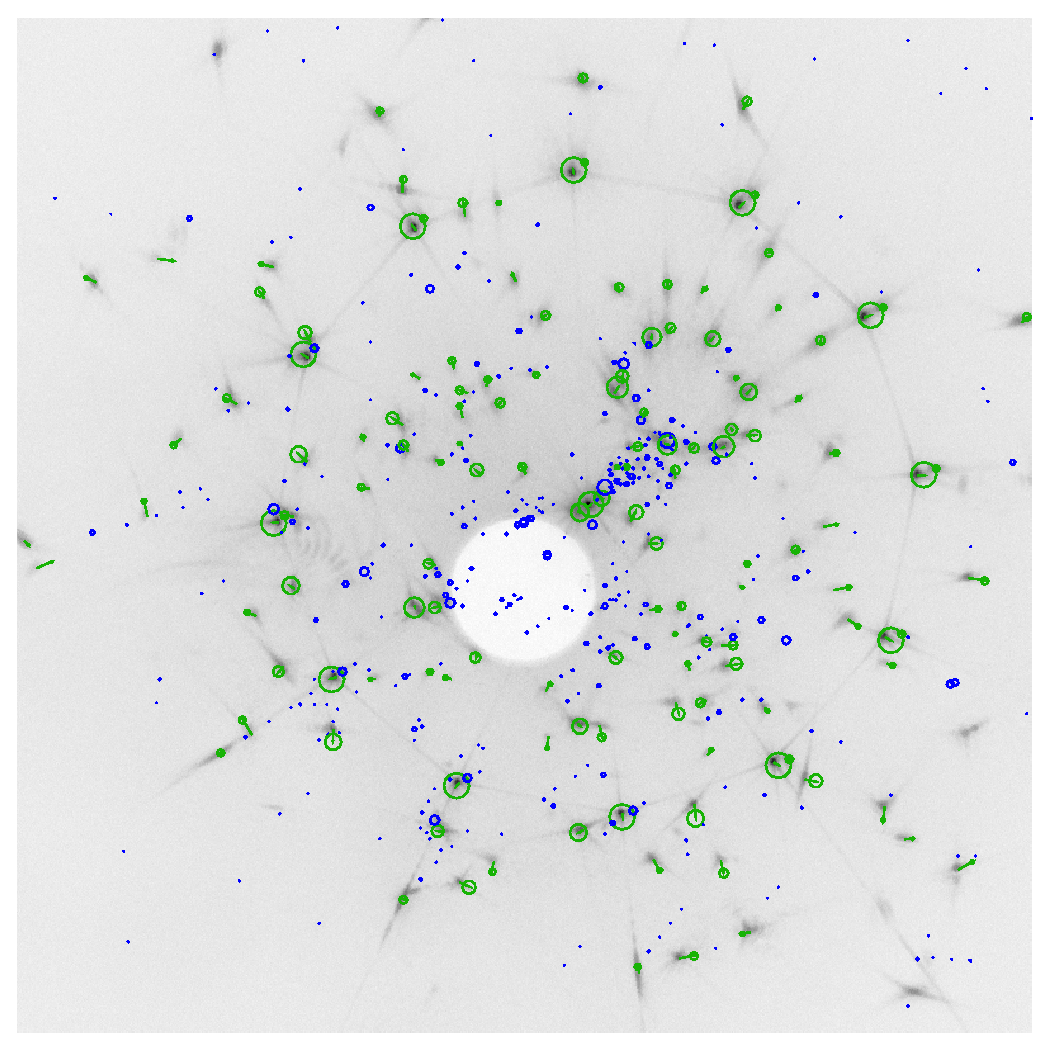
\includegraphics[width=\textwidth]{kores_faze_4.eps}
    \caption[Vzdálenost korespondujících svazků - konečná fáze.]{Vzdálenost korespondujících svazků po optimalizaci náklonu faset podle všech korespondujících svazků. Kružnice znázorňují referenční svazky. Čím vyšší je zářivý tok svazku, tím vyšší je poloměr kružnice. Vektory směřují od obrazu měřeného svazku k obrazu korespondujícího referenčního svazku. Zelenou barvou jsou zobrazeny korespondence použité při optimalizaci parametrů kamene. Modrou barvou jsou zobrazeny referenční svazky, pro které nebyl nalezen měřený svazek. Detail na střední část snímku. }
 \label{fig: kores_faze_2}
 \end{figure}
 
 \clearpage
\part{Klasifikace příznaků}

Nalézt korespondující dvojice pozorovaných a simulovaných svazků pouze pomocí směru svazků je prakticky nemožné. Proto se pokusíme využít další příznaky, které nám pomohou eliminovat nesprávné korespondence. Víme, že u pozorovaných svazků můžeme kromě směru určit zářivý tok a detekovat ocásky (kapitola \ref{sec:beam parameters}).   

Prozkoumáme parametry pozorovaných a simulovaných svazků s cílem navrhnout jednoduchý klasifikátor. Nalezení závislosti parametrů zjednoduší úlohu korespondence svazků.  
\vspace{4mm}

\section{Ground truth}

Abychom mohli hledat závislosti mezi parametry pozorovaných a simulovaných svazků, potřebujeme získat data s korespondujícími svazky. Toho dosáhneme tak, že ručně upravujeme množinu korespondencí a optimalizujeme náklon faset pomocí programu v příloze \ref{sec:handOptim}. Proces ručního přiřazování svazků ukončíme, když nalezneme dostatečně přesný sklon faset. Takto nalezené korespondence považujeme za správné.     

Ručně určené korespondence označujeme výrazem "\textit{ground truth}" podobně jako v oblasti strojového učení, kde slouží jako přesná data v trénovací množině pro určení statistických modelů. Použití výrazu "\textit{ground truth}" je ovšem v našem případě sporné, neboť určení množiny korespondencí závisí na osobě, která tato úlohu provádí. To, co v našem případě označujeme jako "\textit{ground truth}", je množina, o které se domníváme, že by měla obsahovat správné korespondence svazků, ale v našem případě nemůžeme s naprostou jistotou tvrdit, že tomu tak je. 

\section{Změna zářivého toku se změnou parametrů kamene}
\label{sec: zmena_tok }

	Chceme zjistit, jak je zářivý tok svazků závislý na změně parametrů faset. 

	Máme k dispozici korespondující svazky z měření 10 různých kamenů typu \textit{viva12}. Při určení "\textit{ground truth}" jsme zároveň odhadli skutečné sklony faset a matematické modely kamenů. Vezmeme si postupně každý z těchto modelů a měníme náklon normály vybrané fasety o jeden stupeň ve čtyřech kolmých směrech. Nakonec normálu vrátíme zpět na původní hodnotu. Takto nakloníme normály všech 14 faset kamene. Dostaneme 4$\times$14 modelů kamene plus jeden původní. 
	
	Nakloněním normály fasety vznikne nový model kamene. Pro tento model pomocí LADOKu  vypočítáme parametry svazků. Pokud se zářivý tok svazku od původního modelu změnil, zapamatujeme si jeho hodnotu. Pro jednotlivý svazek dostaneme vektor hodnot zá\-ři\-vé\-ho toku $\vv{\phi}_e$. 
	
	 Abychom mohli porovnat změnu zářivého toku, který se může u svazků řádově lišit, vyjádříme změnu toku pomocí variačního koeficientu $c_v$. Variační koeficient je výsledkem podílu směrodatné odchylky a střední hodnoty vektoru $\vv{\phi}_e$. 
	 
	 \begin{equation}	 
	 c_v = \frac{\sigma(\vv{\phi}_e)}{E(\vv{\phi}_e)}
	 \end{equation}
	 
Určíme variační koeficient simulovaných svazků a výsledek ze všech 10 kamenů zaneseme do histogramu na obr. \ref{fig: flux_var_coeff}. V histogramu vidíme, že existuje nezanedbatelný počet svazků, pro které změna náklonu fasety o \SI{1}{\degree} znamená změnu zářivého toku o více než polovinu původní hodnoty. Je zřejmé, že obdobně se bude měnit zářivý tok svazků při posunu fasety. 

 Výsledek naznačuje, že nebude snadné nalézt funkci, která by definovala vztah mezi zářivým tokem simulovaných a pozorovaných svazků.  

\begin{figure}[htps]
\centering
\includegraphics[width = 0.8\textwidth]{flux_var_coeff.eps}
\caption{Histogram variačního koeficientu zářivého toku svazků pro data z 10 snímků různých kamenů typu \textit{viva12}.}
\label{fig: flux_var_coeff}
\end{figure}



\section{Závislost zářivého toku}
\label{sec: tok_zavislost}
	Broušený kámen je ozářen laserovým svazkem o vlnové délce \SI{670}{\nano\metre}. Při průchodu svě\-tel\-né\-ho svazku kamenem se část záření absorbuje a přemění se na teplo. Absorpce záření závisí na odstínu kamene, proto si vybereme kameny stejného odstínu. V našem případě zvolíme odstín \textit{Hyacint}, který se vyznačuje nízkou absorpcí zdrojového svazku. 
	
	Korespondující svazky jsme určili pro 4 kameny odstínu \textit{Hyacint}, kde každý kámen byl 3$\times$ s různou rotací umístěn do měřicí soustavy. S korespondencemi z 12 snímků pracujeme jako s celkem a dostaneme množinu uspořádaných dvojic pozorovaných a simulovaných svazků. 
	
	Pozorované svazky charakterizuje zářivý tok $\vv{\phi}_{e_m}$ a simulované svazky zářivý tok $\vv{\phi}_{e_r}$. Cílem je nalézt funkci $h$, pro kterou
	
	\begin{equation}	
		\phi_{e_m} = h \left( \phi_{e_r} \right) \,.
		\label{eq: fi_fi}
	\end{equation}

Abychom mohli porovnat data z více měření, vyjádříme si zářivý tok pozorovaných svazků jako jejich poměr ku součtu zářivého toku všech pozorovaných svazků v jednotlivém snímku. 

Závislost $\phi_{e_m} =  f\left( \phi_{e_r} \right)$ vyneseme do grafu na obr. \ref{fig: flux_depend2}, kde jsou vykresleny pouze svazky s variačním koeficientem $c_v$ menším než $0.5$.

\begin{figure}[htps]
\centering
\includegraphics[width = 0.8\textwidth]{flux_depend2.eps}
\caption[Závislost zářivého toku simulovaných a pozorovaných svazků.]{Závislost velikosti zářivého toku pozorovaných svazků na velikosti zářivého toku simulovaných svazků. Zobrazeny jsou pouze svazky s variačním koeficientem zářivého toku větším než $0.5$. Výsledky pro odstín \textit{Hyacint}. Vynechány jsou svazky třídy \textbf{3B}. Přímky $\mathbf{b_0}$ a $\mathbf{b_1}$ naznačují, že rozptyl zářivého toku pozorovaných svazků roste s velikostí zářivého toku simulovaných svazků. Svazky třídy \textbf{3A} jsou zvýrazněny.}
\label{fig: flux_depend2}
\end{figure}

\begin{figure}[htps]
\centering
\includegraphics[width = 0.8\textwidth]{flux_depend1.eps}
\caption[Závislost zářivého toku simulovaných a pozorovaných svazků - detail.]{Detail obrázku \ref{fig: flux_depend2}. Vynechány jsou svazky třídy \textbf{3A} a \textbf{3B}. Svazky třídy \textbf{1A} jsou zvýrazněny.}
\label{fig: flux_depend1}
\end{figure}

  Výsledek není příliš optimistický. Data v grafu jsou příliš rozptýlena na to, abychom mohli nalézt spolehlivou funkci popisující závislost \ref{eq: fi_fi}. Důvodů může být hned několik. 

Víme, že v modelu kamene nejsou postihnuty všechny skutečnosti ovlivňující velikost zářivého toku stop. Můžeme zmínit například to, že v modelu není zahrnuta čistota materiálu, která nemusí a prakticky ani není v celém materiálu konstantní. Nedokonalé proleštění fasety ovlivňuje rozptylové parametry světelného svazku. Změna parametrů fasety vede ke změně plochy fasety, tedy i ke změně plochy svazku, který je omezen hranou této fasety. Malá změna parametrů fasety může vést k velké změně zářivého toku svazku, což jsme si ukázali v kapitole \ref{sec: zmena_tok }. Tyto a další vlastnosti v konečném důsledku vyústí v chybu údaje na ose $y$ v grafu na obr. \ref{fig: flux_depend2}.

Na druhé straně musíme počítat s nejistotou určení zářivého toku pozorovaných svazků vznikající při výpočtu parametrů svazků z obrazu. Mezi zásadní problémy patří šum, pře\-krý\-vá\-ní stop, difuzní odrazivost svazků či odhad pozadí snímku.  


\section{Závislost parametrů ocásků}

	Zajímáme se o to, jak může přispět znalost ocásků pozorovaných a simulovaných svazků k nalezení korespondující dvojice.  

  Korespondující ocásky nalezeme pomocí jednoduchého algoritmu založeného na podobnosti směru ocásků korespondujících stop. Takto nalezené korespondence zkontrolujeme a případně upravíme. Máme k dispozici data korespondujících ocásků pro 25 snímků celkem deseti kamenů \textit{viva12}. 
	
	Ocásky parametrizujeme pomocí velikosti $\rho$ a směrového úhlu $\phi$. Z korespondujících ocásků získáme parametry pozorovaných ocásků $\vv{\rho}_m$ a $\vv{\varphi}_m$ a k nim odpovídající simulované parametry $\vv{\rho}_r$ a $\vv{\varphi}_r$.
	

\subsection{Směrový úhel}
 U směrového úhlu potřebujeme vědět, do jaké míry souhlasí směr pozorovaného a směr simulovaného ocásku. Vypočítáme rozdíl směrových úhlů $\Delta\vv{\phi}$ a vyneseme do grafu \ref{fig: tail_depend1} rozložení pravděpodobnosti.  
 
 \begin{equation}
 \Delta\vv{\phi} = \vv{\varphi}_m - \vv{\varphi}_r
 \end{equation}
  
\begin{figure}[htps]
\centering
\includegraphics[width = 0.8\textwidth]{tails_gauss.eps}
\caption[Odhad pravděpodobnostní funkce rozdílu směrového úhlu mezi pozorovanými a simulovanými ocásky.]{Odhad pravděpodobnostní funkce rozdílu směrového úhlu mezi pozorovanými a simulovanými ocásky. Aproximace Gaussovou křivkou s parametry $\sigma = $ \SI{4.43}{\degree} a $\mu = $ \SI{-0.86}{\degree}. }
\label{fig: tail_depend1}
\end{figure}

Pravděpodobnostní rozdělení na obr. \ref{fig: tail_depend1} lze aproximovat Gaussovu funkcí

\begin{equation}
f(\Delta\varphi) = \frac{1}{\sigma\sqrt{2\pi}}\cdot e^{-\frac{\left(\Delta\varphi - \mu\right)^2}{2\sigma^2}}\, 
\end{equation}
s rozptylem $\sigma =  $ \SI{4.43}{\degree} = \SI{0.077}{\radian} a střední hodnotou $\mu = $ \SI{-0.86}{\degree} = \SI{-0.15}{\radian}. Tato funkce může sloužit jako základ pro určení podobnosti ocásků.   

\subsection{Velikost}
	Vykreslili jsme si závislost velikosti pozorovaných ocásků na velikosti simulovaných ocásků. Graf na obr. \ref{fig: tail_depend2} obsahuje pouze náhodně vybrané vzorky závislosti $\rho_m = f(\rho_r)$, kde $\rho_m$ a $\rho_r$ jsou normované velikost pozorovaných, resp. simulovaných ocásků. Zdá se, že mezi velikostí pozorovaných a simulovaných ocásků není takřka žádná souvislost. Nejsme schopni nalézt funkci $f$, která by popisovala závislost $\rho_m = f(\rho_r)$.
	
	\begin{figure}[htps]
\centering
\includegraphics[width = 0.8\textwidth]{tails_rho.eps}
\caption[Závislost velikosti simulovaných a pozorovaných ocásků.]{Závislost velikosti pozorovaných ocásků $\rho_m$  na velikosti  simulovaných ocásků $\rho_r$ pro náhodně vybranou podmnožinu korespondujících ocásků.}
\label{fig: tail_depend2}
\end{figure}

\clearpage
\part{Automatická optimalizace - algoritmy}
	Uvedeme algoritmy využité pro hledání korespondencí měřených a referenčních svazků a popíšeme jejich aplikaci pro automatické určení náklonu faset broušených kamenů. 
	Předtím, než se začneme zabývat navrženými přístupy, je třeba sjednotit značení jednotlivých parametrů svazků. 
	
	Referenční svazky dělíme do tří množin. 
	
	\begin{tabular}{l l}
	$\mathcal{R}_c$ & - uspořádaná $r_c$-tice svazků, pro které byl nalezen korespondující měřený svazek,\\
	$\mathcal{R}$   & - uspořádaná $r$-tice svazků, ke kterým můžeme přiřadit korespondující měřený savek, \\
	$\mathcal{R}_o$ & - uspořádaná $r_o$-tice svazků, které není možné přidat do množiny korespondencí $\mathcal{C}$.  \\
	\end{tabular}	

Pro tyto množiny platí $\mathcal{R}_c \cap \mathcal{R} = \emptyset$, $\mathcal{R} \cap \mathcal{R}_o = \emptyset$, $\mathcal{R}_c \cap \mathcal{R}_o = \emptyset$, kde $\mathcal{R} = \left(\mathrm{R}_1 ,\,\dots,\, \mathrm{R}_r\right)$. Dále definujeme uspořádanou $r^\prime$-tici $\mathcal{R}^\prime = \mathcal{R} \cup \mathcal{R}_o$. $r^\prime = r +r_o $.
	
	Podobně dělíme měřené svazky na $\mathcal{M}_c$, $\mathcal{M}$, $\mathcal{M}_o$ a $ \mathcal{M}^\prime$, kde $\mathcal{M} = \left(\mathrm{M}_1 ,\,\dots,\, \mathrm{M}_m\right)$.
	 
	 Algoritmy pracují s informacemi o směru, obrazu a zářivém toku $\phi_e$ svazků. Směr vyjadřujeme pomocí azimutu $\alpha$ a elevace $\varepsilon$. Polohu obrazu svazku určuje $x$-ová a $y$-ová souřadnice.
	
	 Parametry referenčních svazků označujeme $\vv{\alpha}_{r}$, $\vv{\varepsilon}_{r}$, $\vv{\phi}_{e_{r}}$, $\vv{x}_r$  a $\vv{y}_r$. Pro měřené svazky platí označení $\vv{\alpha}_{m}$, $\vv{\varepsilon}_{m}$, $\vv{\phi}_{e_{m}}$, $\vv{x}_m$  a $\vv{y}_m$. Platí, že $\vv{\alpha}_{r} = \alpha_{r}\left(\mathcal{R}\right)$, $\vv{\alpha}_{m} = \alpha_{m}\left(\mathcal{M}\right)$ apod. 

Množinu korespondujících svazků značíme $\mathcal{C}$. Jednotlivá korespondence $\mathrm{C}_i$ je uspořádaná dvojice $\left(\mathrm{R}_j,\,\mathrm{M}_k \right)$, $\mathrm{C}_i \subseteq \mathcal{C}$. $\alpha_{r}(\mathrm{C}_i)$ označuje azimut referenčního svazku $\mathrm{R}_j$, kde $\mathrm{R}_j \subset \mathrm{C}_i$ a $\alpha_{r}(\mathcal{C})$ vektor $\left(\alpha_{r}(\mathrm{C}_1),\,\dots,\,\alpha_{r}(\mathrm{C}_n)\right)$, kde $n$ je počet uspořádaných dvojic v množině $\mathcal{C}$.
	
	 

\section{Použité algoritmy}
	Korespondence hledáme buď pro specifickou třídu třídu svazků nebo pro svazky, které splní požadované parametry. 

\subsection{Korespondence svazků třídy \textbf{1A}}
\label{sec: 1A}

Víme, že svazky třídy \textbf{1A} se odráží od faset \textbf{UF1} - \textbf{UF2}. Úhlová odchylka normály referenční fasety skutečné normály se projeví dvojnásobnou úhlovou odchylkou referenčního svazku od měřeného. Očekáváme, že rozdíl mezi referenčními a reálnými parametry faset není příliš velký. Proto lze očekávat, že měřené svazky třídy \textbf{1A} budou mít velmi podobný směr jako referenční. Přibližně tedy známe směr těchto svazků.

V blízkém okolí stop třídy \textbf{1A} se mohou nacházet pouze stopy s řádově nižším zářivým tokem. Tato vlastnost je zajištěna geometrií kamene \textit{viva12} a provedením experimentu. Pokud známe zářivý tok stop, můžeme v obraze snadno nalézt svazek třídy \textbf{1A}. 

\paragraph{Parametry algoritmu}
\hspace{1mm}
	 
	 \begin{tabular}{l l}
	 $d_{max}$ & - kvadrát maximální vzdálenosti měřeného svazku od referenčního,\\
	 $n_{min}$ & - minimální počet měřených svazků, v blízkém okolí referenčního svazku, s nižším zářivým tokem než zářivý tok potenciálního korespondujícího měřeného svazku. \\
	 \end{tabular}
	
\paragraph{Popis algoritmu} 

\begin{enumerate}
\item Definujeme proměnné $\alpha_{c} = 0$, $\varepsilon_{c} = 0$, $\mathcal{C} = \emptyset$, $\mathcal{C}_{l} = \emptyset$.

\item $i = 0$.

\item Vypočítáme kritérium hodnotící vzdálenost mezi svazky 

$\vv{d} = (\alpha_{r}(\mathrm{R}_i)\cdot\vv{\mathbf{1}}-\vv{\alpha}_{m}-\alpha_{c}\cdot\vv{\mathbf{1}})^2 + (\varepsilon_{r}(\mathrm{R}_i)\cdot\vv{\mathbf{1}}-\vv{\varepsilon}_{m}-\varepsilon_{c}\cdot\vv{\mathbf{1}})^2 $.

\item Vybereme uspořádanou $k$-tici svazků $\mathcal{N}$ z $\mathcal{M}$, která odpovídá rostoucí posloupnosti $\vv{d}$ a omezení na $\vv{d} < d_{max}$. $\mathcal{N}_1 \sim \argmin(d)\,$ tak, že $\mathcal{N} = \left(\mathrm{M}_a ,\,\dots,\, \mathrm{M}_b \right)$, kde $a = \argmin(\vv{d})$ a $b = \argmin\left(\dfrac{1}{\vv{d}-d_{max}}\right)$. Dále bude platit, že  $\mathrm{N}_1 = \mathrm{M}_a$ a $\mathrm{N}_k = \mathrm{M}_b$ apod. 

\item Nalezneme uspořádanou $k$-tici $\mathcal{O}$ takovou, že $\mathcal{O} = \left(\mathrm{N}_1 ,\,\mathrm{N}_e,\,\mathrm{N}_f ,\,\dots,\, \mathrm{N}_g \right)$, kde\\$e = \argmin\left( \phi_{e_{m}}\left(\mathrm{N}_1 \right),\, \phi_{e_{m}}\left(\mathrm{N}_2 \right)  \right)$, $f = \argmin\left( \phi_{e_{m}}\left(\mathrm{N}_1 \right),\, \phi_{e_{m}}\left(\mathrm{N}_2 \right),\, \phi_{e_{m}}\left(\mathrm{N}_3 \right)   \right)$ a \\  $g = \argmin\left( \phi_{e_{m}}\left(\mathrm{N}_1 \right),\,\dots,\, \phi_{e_{m}}\left(\mathrm{N}_k \right)  \right)$.  

\item Určíme vektor $\vv{n_\mathcal{O}}$ o velikosti $k$ udávající četnost prvků z množiny $\mathcal{N}$ v množině $\mathrm{O}$. Pokud $\mathrm{O}_q = \mathcal{O}_s$, tak $n_{\mathcal{O}}(q) = n_{\mathrm{O}}(s)$, pro $q = \lbrace1,\,\dots,\,k \rbrace$ a podobně $s = \lbrace 1,\,\dots,\,k \rbrace$.

\item Určíme minimální $l$, které splňuje alespoň jednu z podmínek $n_{\mathcal{O}}(l) > n_{min}$  a $l = k$. Do množiny $\mathcal{C}$ přidáme korespondenci $\left(\mathrm{R}_i,\,\mathrm{N}_l \right)$.

\item Pokud $i \neq r$, tak $i = i+1$ a opakujeme body 3) až 7).

\item Pokud $\mathcal{C}_{l} \neq \mathcal{C}$, vypočítáme korekční parametry $\alpha_{c} = median(\alpha_{r}(\mathcal{C})-\alpha_{m}(\mathcal{C}))$, \\ $\varepsilon_{c} = median(\varepsilon_{r}(\mathcal{C})-\varepsilon_{m}(\mathcal{C}))$, položíme $\mathcal{C}_{l}$ rovno $\mathcal{C}$  a opakujeme body 2) až 8).

\item Z $\mathcal{C}$ odstraníme prvky, ve kterých se obraz referenčního svazku nachází mimo obraz stínítka.

\item Optimalizujeme náklon kamene (kapitola \ref{sec:Optimalizace_crit}).

\item Podle výsledku optimalizace upravíme model kamene a přepočítáme parametry referenčních svazků. Opakujeme bod 1) až 10). V příští iteraci tento bod vynecháme. 

\item Z $\mathcal{C}$ odstraníme prvky, ve kterých se obraz referenčního svazku nachází mimo obraz stínítka.

\end{enumerate}
\newpage
\subsection{Korespondence svazků třídy \textbf{3A}}	
\label{sec:3A}
	Po optimalizaci podle třídy \textbf{1A} máme dobře odhadnuté parametry faset \textbf{UF1} - \textbf{UF12}. Pomocí rotace a náklonu kamene odhadneme přibližně parametry faset \textbf{TOP} a \textbf{BOT}. Podstatné je, že svazek třídy \textbf{3A} dopadá na tabulku \textbf{TOP} pod výrazně menším úhlem, než je kritický úhel. To zajišťuje přijatelnou citlivost směru svazků na změnu parametrů dopadových faset. 
	
	Referenční svazky třídy \textbf{3A} mají po třídě \textbf{3B} druhý nejvyšší zářivý tok. Ostatní třídy se vyznačují řádově nižším zářivým tokem. Podle zářivého toku $\phi_{e_r}$  lze tedy snadno oddělit svazky se třemi dopadovými fasetami od ostatních svazků. Referenčních svazků třídy \textbf{3A} a \textbf{3B} je celkem 13. Často nastává situace, že svazek třídy \textbf{3B} nedetekujeme, protože je jeho obraz zakrytý podstavcem na kámen. 
	
	Separaci podle zářivého toku  však nelze s jistotou použít u měřených svazků. Pokud dojde k překrytí obrazu svazků jiných tříd, může být zářivý tok tohoto shluku větší. Spolehlivý způsob, jak oddělit měřené svazky třídy \textbf{3A} a \textbf{3B} od ostatních, je porovnat maximální úrovně jasu v obrazech svazků.  
	
	Další vlastnost, která dobře charakterizuje svazky třídy \textbf{3A} jsou dlouhé a intenzivní ocásky. Při hledání korespondencí můžeme využít párování svazků podle charakteru ocásků (kapitola \ref{sec: korespondence_ocasky}). Výhodou algoritmu je to, že dokážeme za vhodného nastavení nalézt korespondující svazky, a to i v případě vysokých směrových odchylek svazků. Nevýhodou je necitlivost na ostatní parametry svazků. 

\paragraph{Popis algoritmu} 

\begin{enumerate}
	\item Redukujeme počet měřených svazků a vytvoříme uspořádanou 13-tici $\mathcal{M}$ obsahující prvních 13 měřených svazků s nejvyšší hodnotou jasu v obraze. 

	\item Podle podobnosti ocásků nalezneme počáteční odhad množiny korespondencí $\mathcal{C}$ (kapitola \ref{sec: korespondence_ocasky})). Parametry algoritmu: $\sigma = 0.2$, $L_{min} = 2$, $\Delta\alpha_{max} = 35^\circ$, $\Delta\varepsilon_{max} = 15^\circ$.
	
	\item Uvolníme pouze parametry faset \textbf{TOP} a \textbf{BOT}. V tomto kroku prohlásíme parametry těchto dvou faset za totožné a optimalizujeme parametry uvolněných faset (kapitola \ref{sec:Optimalizace_crit}). Pokud neznáme dostatečně přesně index lomu kamene optimalizujeme také index lomu. 
	
	\item Podle výsledku optimalizace upravíme model kamene a přepočítáme parametry referenčních svazků. Pro finální odhad množiny korespondencí $\mathcal{C}$ použijeme algoritmus v kapitole \ref{sec: 1A} od bodu 1) do bodu 10). $\mathcal{R}$ bude uspořádaná 24-tice referenčních svazků třídy \textbf{1A} a \textbf{3A}. $\mathcal{M}$ bude obsahovat všechny měřené svazky.  
	
	\item K optimalizovaným parametrům přidáme parametry faset \textbf{UF1} až \textbf{UF12} a optimalizujeme. 
		
\end{enumerate}

\newpage
\subsection{Korespondence svazků třídy \textbf{5D}}
\label{sec:5D}
	Svazky třídy \textbf{5D} můžeme v obraze pozorovat, pokud existuje úhlová odchylka mezi fasetou \textbf{TOP} a \textbf{BOT}. Předpokládáme, že pokud nějaká odchylka vznikne, bude max. \SI{1}{\degree}. Také předkládáme, že normály faset \textbf{UF1} až \textbf{UF12} nejsou vůči pravidelnému tvaru \textit{vivy12} příliš vychýleny.
	
	Podstatné je, že známe polohu svazků třídy \textbf{3A}. Za výše uvedených okolností lze pozorovat vzor určující vzájemnou polohu dvojice svazků třídy \textbf{3A} a \textbf{5D}, které mají v seznamu stejné dopadové fasety např. dvojice (UF1-TOP-BOT, UF1-TOP-BOT-TOP-BOT). Vzájemnou polohu mezi všemi těmito páry lze popsat pomocí polárních souřadnic vzdáleností $\rho$ a úhlem $\varphi$. 
	
	Polohu j-tého měřeného svazku popisujeme souřadnicemi $x_m(\mathrm{M}_j)$ a $y_m(\mathrm{M}_j)$. Měřené svazky rozdělíme na uspořádanou $n$-tici $\mathcal{N}$ obsahující 12 svazků třídy 3A a uspořádanou $o$-tici $\mathcal{O}$ obsahující zbylé svazky. 

\paragraph{Parametry algoritmu}
\hspace{1mm}

	 \begin{tabular}{l l}
	 $\rho_{max}$ & - maximální vzdálenost obrazu svazků třídy \textbf{3A} a \textbf{5D} v pixelech,\\
	 $\Delta\rho$ & - maximální absolutní odchylka úhlu v obraze mezi párem svazků třídy \textbf{3A} a \textbf{5D},\\
	 $\Delta\varphi$ & - maximální absolutní odchylka vzdálenosti v obraze mezi párem svazků třídy \textbf{3A} a \textbf{5D},\\
	 $p_{min}$ & - minimální počet nalezených dvojic.\\
	 \end{tabular}

\paragraph{Algoritmus}

\begin{enumerate}
\item Vypočítáme Euklidovu vzdálenost obrazů jednotlivých svazků

$\rho_{j,k} = \sqrt{\left( x_m(\mathrm{N}_j) - x_m(\mathrm{O}_k) \right)^2 + \left( y_m(\mathrm{N}_j) - y_m(\mathrm{O}_k) \right)^2}$ 

pro $j = \lbrace 1,\,\dots,\,n \rbrace$ a $k = \lbrace 1,\,\dots,\,o \rbrace$. 

Směrový úhel určíme podle vztahu $\varphi_{j,k} = \arctan\dfrac{y_m(\mathrm{N}_j) - y_m(\mathrm{O}_k)}{x_m(\mathrm{N}_j) - x_m(\mathrm{O}_k)}$.

\item Vybereme svazky vzdálené méně než $\rho_{max}$ a dostaneme vektor vzdáleností $\vv{\rho}$ a směrových úhlu $\vv{\varphi}$.

$\lbrace \varphi_{j,k} \subseteq \vv{\varphi},\,\rho_{j,k} \subseteq \vv{\rho}\,|\,\, \rho_{j,k} < \rho_{max} \rbrace$ pro $j = \lbrace 1,\,\dots,\,n \rbrace$ a $k = \lbrace 1,\,\dots,\,o \rbrace$,
 
 kde  $\vv{\varphi} = (\varphi_{{j_1},{k_1}},\,\dots,\,\varphi_{{j_s},{k_s}}) = (\varphi_{1},\,\dots,\,\varphi_{s})$ a $\vv{\rho} = (\rho_{{j_1},{k_1}},\,\dots,\,\rho_{{j_s},{k_s}}) = (\rho_{1},\,\dots,\,\rho_{s})$. 

\item Definujeme funkce $g(x)\rightarrow \begin{cases}
1, & |x| < \Delta\rho\\
0, & jinak
\end{cases}\,, \hspace{4mm}h(x) \rightarrow \begin{cases}
1, & |x| < \Delta\varphi\\
0, & jinak
\end{cases}$. 

Pro vektor $\vv{x}$ délky $n$ platí $g(\vv{x}) = \left(g(x_1),\,\dots,\,g(x_n)\right)$ a $h(\vv{x}) = \left(h(x_1),\,\dots,\,h(x_n)\right)$.

 Nechť $a = \underset{{q = \lbrace1,\,\dots,\,s\rbrace}}{\argmax}\,\, \overset{s}{\underset{{i = 1}}{\sum}} g\left(\varphi_i-\varphi_q\right)$, \hspace{4mm} $b = \underset{{q = \lbrace1,\,\dots,\,s\rbrace}}{\argmax}\,\, \overset{s}{\underset{{i = 1}}{\sum}} h\left(\rho_i-\rho_q\right)$, potom 

$\vv{\upsilon} = g\left(\vv{\varphi} - \varphi_a\cdot\vv{\mathbf{1}} \right) + h\left(\vv{\rho} - \rho_b\cdot\vv{\mathbf{1}} \right)$.


\item Nalezeme množinu potenciálních korespondencí $\mathcal{C^\prime}$. $\lbrace \left(\mathrm{R}_t,\mathrm{O}_{k_q}\right) \subseteq \mathcal{C^\prime} \,|\,\, \upsilon_q > 1 \rbrace$, pro $q = \lbrace1,\,\dots,\,s\rbrace$, kde $R_t$ je referenční svazek třídy \textbf{5D} se stejným seznamem dopadajících faset jako měřený svazek $\mathrm{N}_{j_q}$.

\item Pokud $\mathcal{C^\prime}$ obsahuje alespoň $p_{min}$ prvků, přidáme $\mathcal{C^\prime}$ do množiny korespondencí $\mathcal{C}$.

 
\end{enumerate}

\newpage
\subsection{Korespondence svazků podle polohy v obraze a zářivého toku}
\label{sec: poloha_tok}
	Tento algoritmus se snaží o to nalézt dvojici svazků, které se promítnou na podobnou pozici v obraze a mají vysoký zářivý tok. Snažili jsme se nalézt funkci, která by charakterizovala závislost mezi zářivým tokem $\phi_{e_{r}}$ referenčních stop a zářivým tokem $\phi_{e_{m}}$ měřených stop. Jednoduchou funkci jsme však nenašli. Ke korespondenci svazků budeme místo absolutního zářivého toku využívat jeho relativní velikosti vzhledem k ostatním svazkům v blízkém okolí. 

\paragraph{Parametry algoritmu}
\hspace{1mm}
	 
	 \begin{tabular}{l l}
	 $d_{m_{max}}$ & - maximální vzdálenost měřených svazků v pixelech  $d_{m_{max}} = $ \SI{80}{\px},\\
	 $d_{r_{max}}$ & - maximální vzdálenost referenčního svazku od měřeného svazku v pixelech $d_{r_{max}} = $ \SI{50}{\px},\\
	 $\mathbf{L}_{max}$ &  - maximální velikost kritéria  $\mathbf{L} \in \mathbb{R}^{r^\prime\times m^\prime}$ pro přidání dvojice svazků do množiny korespondencí $\mathcal{C}$. \\
	 \end{tabular}

\paragraph{Algoritmus}

\begin{enumerate}
\item $j = 1$, $\vv{w}_{m^\prime} = \vv{\mathbf{1}}$, $\vv{w}_{r^\prime} = \vv{\mathbf{1}}$. 

\item Nalezneme 3 svazky $\left(\mathrm{M}^\prime_a,\,\mathrm{M}^\prime_b,\,\mathrm{M}^\prime_c \right) \subset \lbrace \mathcal{M}^\prime\setminus \mathrm{M}^\prime_j\rbrace$ s nejmenší Euklidovou vzdáleností obrazu $\left(d_a,\,d_b,\,d_c\right)$ od svazku $\mathrm{M}^\prime_j$.

$d_a = \sqrt{\left( x_{m}(\mathrm{M}_j^\prime) -  x_{m}(\mathrm{M}_a^\prime) \right)^2 + \left( y_{m}(\mathrm{M}_j^\prime) -  y_{m}(\mathrm{M}_a^\prime) \right)^2}$.

\item Nechť $f(\mathrm{M}^\prime_x)\rightarrow \begin{cases}
\phi_{e_{m}}\left(\mathrm{M}^\prime_x \right), & d_x < d_{m_{max}}\\
1, & jinak
\end{cases}$, $\phi_{e_{m}}(\mathrm{M}^\prime_j) > 1 $ potom 

$\phi_{m^\prime_{max}} = \max\left(\phi_{e_{m}}(\mathrm{M}^\prime_j),\,f(\mathrm{M}^\prime_a),\,f(\mathrm{M}^\prime_b),\,f(\mathrm{M}^\prime_c)  \right)$. 

\item Nastavíme váhy měřených svazků.

 $w_{m^\prime_{q}} = \dfrac{\phi_{max}}{f(\mathrm{M}^\prime_q)}$ pro $q = \lbrace j,\,a,\,b,\,c \rbrace$.
 
\item Nalezneme uspořádanou $s$-tici $\mathcal{S} = (\mathrm{S}_1,\,\dots,\,\mathrm{S}_s)$ referenčních svazků z $\mathcal{R}^\prime$. 

$\lbrace \mathrm{R}^\prime_i \subseteq \mathcal{S}\,|\,\, d_{i,j} < d_{r_{max}}  \rbrace$ pro $i = \lbrace 1,\,\dots,\, r^\prime \rbrace$, kde 

$d_{i,j} = \sqrt{\left( x_{m}(\mathrm{M}_j^\prime) -  x_{r}(\mathrm{R}_i^\prime) \right)^2 + \left( y_{m}(\mathrm{M}_j^\prime) -  y_{r}(\mathrm{R}_i^\prime) \right)^2}$.

\item $w_{r^\prime_j} = max\left( \phi_{e_r}(\mathcal{S}) \right)$.

\item Dokud $j \neq n^\prime$, $j = j+1$ a opakujme body 2) až 6). 

\item Nechť  $g(x)\rightarrow \begin{cases}
x, & x > 1\\
1, & jinak
\end{cases}$, potom můžeme určit kriteriální funkci 

\begin{equation}
\mathbf{L}(i,j) = d_{i,j}\cdot w_{m^\prime_{j}} \cdot g \left(\dfrac{\phi_{r_i}(\mathcal{R}^\prime_i)}{w_{r^\prime_{j}}} \right)\,. 
\label{eq: L_tok}
\end{equation}


\item Potenciální korespondence $\mathcal{C}^\prime$ nalezneme podle vzájemně nejnižší velikosti  kritéria v $\mathbf{L}$, které nepřekročí hodnotu $L_{max}$. Korespondující dvojice $\left(\mathrm{R}^\prime_i,\,\mathrm{M}^\prime_j \right) \subseteq \mathcal{C}^\prime$, pokud\\ $i = \underset{{q = \lbrace1,\,\dots,\,r^\prime\rbrace}}{\argmin}\mathbf{L}(q,j)$, $j = \underset{{q = \lbrace1,\,\dots,\,m^\prime\rbrace}}{\argmin}\mathbf{L}(i,g)$ a  $\mathbf{L}(i,j) < L_{max}$. 

\item Vybereme korespondence z $\mathcal{C}^\prime$, které můžeme přidat do množiny korespondencí $\mathcal{C}$. 

 $\lbrace \mathrm{C}^\prime_l \in \mathcal{C}\,|\,\, \mathrm{C}^\prime_l \subseteq \lbrace\mathcal{R}_f \cup \mathcal{M}_f\rbrace \rbrace$.

 
\end{enumerate}

\newpage
\subsection{Korespondence svazků podle ocásků}
\label{sec: korespondence_ocasky}
		
	Ocásky svazků definujeme pomocí velikosti a směrového úhlu.
	
	Počet ocásků referenčního svazku závisí na počtu stran polygonu, kterým popisujeme tvar svazku. Intenzitu ocásku v simulaci určuje zářivý tok svazku a na velikost hrany, na které ocásek vzniká. 
	
	Velikost $\vv{\xi}_{r}\left(\mathrm{R_i}\right)$ a směrový úhel $\vv{\psi}_{r}\left(\mathrm{R_i}\right)$ ocásků  $i$-tého referenčního svazku $\mathrm{R_i}$ určuje vektor o délce $n_i$.\\
	 $\vv{\xi}_{r}\left(\mathrm{R_i}\right) = \left(\xi_{r_1}\left(\mathrm{R_i}\right),\,\dots,\,\xi_{r_{n_i}}\left(\mathrm{R_i}\right)\right)$, $\vv{\psi}_{r}\left(\mathrm{R_i}\right) = \left(\psi_{r_1}\left(\mathrm{R_i}\right),\,\dots,\,\psi_{r_{n_i}}\left(\mathrm{R_i}\right)\right)$, kde $n_i$ je počet ocásků $\mathrm{R_i}$. 
	
	Detekce ocásků měřeného svazku je popsána v kapitole \ref{sec:tails}. Obecně platí, že v obraze jsou detekovatelné ocásky, pro které byla v odpovídající simulaci vypočítána vysoká intenzita. 
	
	Velikost ocásků $j$-té měřené stopy značíme $\vv{\rho}_{m}\left(\mathrm{M_j}\right)$, směrový úhel $\vv{\varphi}_{m}\left(\mathrm{M_j}\right)$. 
	 
	 Podobnost ocásků hodnotíme podle kritéria, a to především na základě podobnosti směru ocásků. Velikost ocásků určuje váhu jednotlivých příspěvků.
	 
\paragraph{Parametry algoritmu}
\hspace{1mm}
	 
	 \begin{tabular}{l l}
	 $\Delta\alpha_{max}$ & - maximální absolutní odchylka azimutu měřeného svazku od referenčního,\\
	 $\Delta\varepsilon_{max}$ & - maximální absolutní odchylka elevace měřeného svazku od referenčního,\\
	 $\sigma$ & - citlivost kriteriální funkce na úhlovou odchylku ocásků,\\
	 $L_{min}$ &  - minimální velikost kritéria  $\mathbf{L} \in \mathbb{R}^{r\times m}$ pro přidání dvojice svazků do množiny korespondencí $\mathcal{C}$. \\
	 \end{tabular}
	
\paragraph{Algoritmus}

\begin{enumerate}
\item $i = 1$

\item Normujeme velikost referenčních ocásků $\vv{\xi}_r\left( \mathrm{R_i} \right) = \dfrac{\vv{\xi}_r\left( \mathrm{R_i} \right)}{\max \left( \vv{\xi}_r\left( \mathrm{R_i} \right) \right)}\,.$

\item Z referenčních ocásků vybereme pouze ty s dominantní intenzitou a získáme vektor velikost $\vv{\rho}_{r}\left(\mathrm{R_i}\right)$ a směr $\vv{\varphi}_{r}\left(\mathrm{R_i}\right)$ o délce $n_k$.\\ $\lbrace \psi_{r_k}\left(\mathrm{R_i}\right) \subseteq \vv{\varphi}_{r}\left(\mathrm{R_i}\right),\, \xi_{r_k}\left(\mathrm{R_i}\right) \subseteq \vv{\rho}_{r}\left(\mathrm{R_i}\right)\,|\,\, \xi_{r_k}\left(\mathrm{R_i}\right) > \xi_{min} \rbrace$, kde $k =\lbrace 1,\,\dots,\,n_i\rbrace $.

\item Nalezneme uspořádanou $n$-tici $\mathcal{N}$ z měřených svazků $\mathcal{M}$. \\$\lbrace \mathrm{M}_j \subseteq \mathcal{N} \,\,|\,\,|\alpha_r(\mathrm{R}_i) - \alpha_m(\mathrm{M}_j) | < \Delta\alpha_{max},\, |\varepsilon_r(\mathrm{R}_i) - \varepsilon_m(\mathrm{M}_j) | < \Delta\varepsilon_{max} \rbrace$, kde $j =\lbrace 1,\,\dots,\,m \rbrace $.


\item Pokud $ \mathrm{M}_j \subseteq \mathcal{N}$, 

\begin{equation}
\mathbf{L}(i,\,j) = \overset{n_k}{\underset{{k = 1}}{\sum}}\, \overset{n_l}{\underset{{l = 1}}{\sum}}\,\dfrac{1}{\sqrt{2\pi}\, \sigma}\cdot e^{-\dfrac{\left(\varphi_{r_k}(\mathrm{R}_i)- \varphi_{m_l}(\mathrm{M}_j) \right)^2}{2\sigma^2}} \cdot \sqrt{\rho_{r_k}(\mathrm{R}_i)\, \rho_{m_l}(\mathrm{M}_j)}\,,
\label{eq:L_tails}
\end{equation}

  
jinak $\mathbf{L}(i,j) = 0$, pro $j =\lbrace 1,\,\dots,\,m \rbrace $, kde $n_l$ je počet ocásků $\mathrm{M_j}$.
  

\item Pokud $i \neq r$, $i = i+1$ a opakujeme kroky 2) až 5).

\item Korespondující svazky nalezneme podle vzájemně nejvyššího kritéria v $\mathbf{L}$ s minimální velikostí $L_{min}$. Korespondující dvojice $\left(\mathrm{R}_i,\,\mathrm{M}_j \right) \subseteq \mathcal{C}$, pokud  $i = \underset{{q = \lbrace1,\,\dots,\,r\rbrace}}{\argmax}\mathbf{L}(q,j)$,\\ $j = \underset{{q = \lbrace1,\,\dots,\,m\rbrace}}{\argmax}\mathbf{L}(i,g)$ a  $\mathbf{L}(i,j) > L_{min}$. 

\end{enumerate}

\newpage
\section{Automatická optimalizace}
\label{sec: auto}

Náklon kamene určíme při hledání korespondencí svazků třídy \textbf{1A}. 

U jednotlivých algoritmů budeme uvádět použité množiny referenčních $\mathcal{R}$ a měřených $\mathcal{M}$ svazků.  a maximální počet odrazů $n_b$ referenčních svazků při jejich výpočtu na novém modelu. Referenční svazky se přepočítávají vždy, když dojde ke změně parametrů kamene. Dále uvádíme parametry použitých algoritmů. 

Před zahájením optimalizace je třeba změřit zkoumaný kámen a určit parametry kamene $d_{TOP}$, $d_{BOT}$, $h$ a $h_{RF}$ (viz kapitola \ref{sec: parametryVIVA12}). 

Pokud neuvedeme, které fasety optimalizujeme, budou optimalizovány stejné parametry jako v předchozím kroku.

Pokud nalezneme dvojici korespondujících svazků, automaticky ji přidáme do množiny korespondencí $\mathcal{C}$.  

\paragraph{Postup optimalizace}
\begin{enumerate}
\item Detekujeme měřené svazky v obraze a určíme jejich parametry. 

\item Podle naměřených parametrů sestavíme model kamene a vyřešíme referenční svazky jednou dopadovou fasetou. 

\item Požijeme algoritmus uvedený v kapitole \ref{sec: 1A} a  nalezneme korespondence svazků třídy \textbf{1A}. Optimalizujeme nejdříve náklon a rotaci kamene a poté parametry faset \textbf{UF1}-\textbf{UF12}.

$\mathcal{R}$ - referenční svazky třídy \textbf{1A}. $\mathcal{M}$ - všechny měřené svazky. Pro první optimalizaci $n_b= 1$, pro druhou optimalizaci $n_b= 4$. Parametry algoritmu jsou následující $d_{max} =  $ \SI{0.051}{\radian^2}, $n_{min} = 5$.

\item Požijeme algoritmus uvedený v kapitole \ref{sec:3A} a  nalezneme korespondence svazků třídy \textbf{3A}. Optimalizujeme parametry faset \textbf{UF1}-\textbf{UF12}, \textbf{TOP} a \textbf{BOT}, u faset \textbf{TOP} a \textbf{BOT} zachováme rovnoběžnost. 

$\mathcal{R}$ - referenční svazky třídy \textbf{3A}. $\mathcal{M}$ - všechny volné měřené svazky. $n_b= 5$. Parametry algoritmu jsou popsány v  v kapitole \ref{sec:3A}.

\item Nalezneme svazky třídy \textbf{5D} podle algoritmu v \ref{sec:5D}. Pokud je detekce svazků třídy \textbf{5D} neúspěšná, zachováme rovnoběžnost faset \textbf{TOP} a \textbf{BOT} a optimalizujeme parametry faset.

$\mathcal{R}$ - referenční svazky třídy \textbf{5D}. $\mathcal{M}$ - všechny volné měřené svazky. $n_b= 7$. Parametry algoritmu: $\rho_{max} = $ \SI{35}{\px}, $\Delta\rho = $\SI{2.5}{\px},  $\Delta\varphi = $ \SI{0.3}{\radian},   $p_{min} = 5 $.

\item Pokud existují referenční svazky třídy \textbf{3C} nalezneme k nim odpovídající měřené svazky. Použijeme algoritmus pro hledání korespondencí podle ocásků \ref{sec: korespondence_ocasky}. Pokud jsme nalezli nějakou korespondenci, optimalizujeme parametry faset.

$\mathcal{R}$ - referenční svazky třídy \textbf{3C}. $\mathcal{M}$ - všechny volné měřené svazky. $n_b= 7$. Parametry algoritmu: $\Delta\alpha_{max}$ = \SI{2}{\degree} ,$\Delta\varepsilon_{max}$ \SI{5}{\degree}, $\sigma = 0.05$, $L_{min} = 10$.

	Máme množinu korespondujících dvojic svazků $\mathcal{C}$ obsahující svazky třídy \textbf{1A}, \textbf{3A}, \textbf{3C} a \textbf{5D}. Tyto korespondence jsou ve většině případů bezchybné, proto zavedeme referenční množinu korespondencí $\mathcal{C}_{ref} = \mathcal{C}$.    

\item Položíme $C = C_{ref}$. Nalezneme korespondence svazků tříd \textbf{6A}, \textbf{6B}, \textbf{6C} a \textbf{6D}. Postup lze rozdělit na více kroků. 

\begin{enumerate}[label={\alph*)}]
	\item Nalezneme potenciální množinu korespondencí $\mathcal{C}^\prime$. Použijeme algoritmus \ref{sec: poloha_tok} s parametrem  $\mathbf{L}_{max} = 30$.
	
	\item Pro potenciální korespondence $\mathcal{C}^\prime$ vypočítáme kritérium podobnosti $\mathbf{L}$ podle ocásků \ref{eq:L_tails}. Pokud je pro pro danou dvojici svazků kritérium větší než 10, přidáme korespondenci do množiny $\mathcal{C}$. 
	
	\item Pro zbylé referenční svazky tříd \textbf{6A}, \textbf{6B}, \textbf{6C} a \textbf{6D} nalezneme korespondence podle ocásků \ref{sec: korespondence_ocasky}. Nastavení parametrů algoritmu: $\Delta\alpha_{max}$ = \SI{7}{\degree} ,$\Delta\varepsilon_{max}$ \SI{5}{\degree}, $\sigma = 0.05$, $L_{min} = 10$.
\end{enumerate}

\item Nalezneme obraz referenčních svazků třídy \textbf{7C} a \textbf{7D}. Tyto svazky jsou v ideálním případě rovnoběžné. Pokud bude nastavení faset takové, že se tyto svazky dostatečně rozbíhají, pokusíme se k nim nalézt korespondující svazky podle bodu 7a) a 7b). 

\item Pokud v bodě 7) a 8) nalezneme méně než tři korespondující svazky, vybereme volné referenční svazky s $\phi_{e_r} > $ \SI{1}{\permille} a elevací větší než \SI{15}{\degree}. Pro vybrané referenční svazky nalezneme korespondující svazky podle ocásků \ref{sec: korespondence_ocasky} s parametry $\Delta\alpha_{max}$ = \SI{25}{\degree} ,$\Delta\varepsilon_{max}$ \SI{10}{\degree}, $\sigma = 0.2$, $L_{min} = 8$.

\item Optimalizujeme parametry faset a 2$\times$ opakujeme body 7) až 9), po nichž opět proběhne optimalizace faset.  

\item Hledáme korespondence v oblastech, kde je malá hustota měřených svazků.  Nalezneme měřené svazky, které mají v obraze nejbližší sousední měřený svazek dále než \SI{50}{\px}. Vybereme referenční svazky se zářivým tokem minimálně  \SI{0.1}{\permille} a elevací minimálně $\min(\varepsilon_r(\mathcal{C}))$. Pro nalezení korespondencí použijeme algoritmus \ref{sec: poloha_tok} s parametrem $\mathbf{L}_{max} = 50$ a optimalizujeme parametry faset. Opakujeme 2$\times$.

\item Současnou množinu korespondencí budeme uvažovat pouze jako potenciální $\mathcal{C}^\prime = \mathcal{C}$ a ponecháme si pouze referenční korespondence $\mathcal{C} = \mathcal{C}_{ref}$. 

\item Vybereme referenční svazky se zářivým tokem minimálně \SI{0.1}{\permille} a elevací minimálně \\ $\min\left( \varepsilon_r( \lbrace\mathcal{C} \cup \mathcal{C}^\prime\rbrace ) \right) - $ \SI{3}{\degree}. Svazky spárujeme pomocí algoritmu \ref{sec: poloha_tok} s parametrem $\mathbf{L}_{max} = 20$.

\item Bod 13) 2$\times$ opakujeme a poté optimalizujeme parametry faset. 

\item Určení korespondencí a optimalizaci podle bodů 12), 13) a 14) dvakrát a dostaneme konečný výsledek  náklonu faset broušených kamenů.

\end{enumerate}

\clearpage
\part{Ověření správnosti korespondencí}	
	
	Máme k dispozici algoritmy, pomocí kterých jsme schopni nalézt korespondující svazky. U~některých, zvlášť u algoritmů v kapitole  \ref{sec: korespondence_ocasky} a \ref{sec: poloha_tok}, můžeme kromě správných korespondencí nalézt řadu falešných  dvojic svazků.
	
	Chceme nalézt metodu schopnou rozhodnout, zda jsou korespondence správné či nesprávné. 
	\vspace{4mm}
	
\section{Množiny korespondencí}
Přicházíme s nápadem rozdělit množiny na čtyři disjunktní množiny.

	\begin{itemize}
	\item \textbf{Optimalizované} -  Do množiny optimalizovaných korespondencí patří korespondence, o kterých jsme si velmi jisti, že jsou správné. Tato množina korespondencí určuje model kamene. 
	
	\item \textbf{Kriteriální} - Kriteriální množina korespondencí složí k výpočtu hodnotícího kritéria. Do této množiny patří, stejně jako do množiny optimalizovaných korespondencí, spolehlivě určitelné korespondence.  
	
	\item \textbf{Kandidátské} - Korespondence, o kterých chceme rozhodnout, zda jsou či nejsou správné.  
	
	\item \textbf{Ostatní} - Korespondence nehodící se ani do jedné z předchozích množin. Typicky svazky příliš vzdálené a svazky s nízkým zářivým tokem.  
\end{itemize}		
	
\section{Rozhodovací algoritmus}
	Množina optimalizovaných korespondencí určujme model kamene. Pro tento model je pro kriteriální množinu korespondencí vypočítáno optimalizační kritérium z rovnice \ref{eq: opt_criter} (dále pouze jako \textit{kritérium}) a určen jeho součet $\varepsilon_0 = \sum\vec{\varepsilon}$.
	 
	Vybereme jednu korespondenci z množiny kandidátů a přidáme ji do množiny optimalizovaných korespondencí. Podle množiny optimalizovaných korespondencí odhadneme nový model kamene. Na tomto modelu  vypočítáme srovnávací \textit{kritérium} pro množinu kriteriálních korespondencí $\varepsilon_c = \sum\vec{\varepsilon}$. 
	
	Změna optimalizačního kritéria je potom 
	
	\begin{equation}
	\Delta\varepsilon  = \varepsilon_0 - \varepsilon_c\,.
	\end{equation}
	
	Pokud je $\Delta\varepsilon  > \varepsilon_t$, kde $\varepsilon_t$ je rozhodovací práh, prohlásíme tuto korespondenci za správnou a ponecháme v množině optimalizovaných korespondencí. V opačném případě korespondenci odstraníme.
	
	Čekali bychom, že optimální práh $\varepsilon_t$ by mohl být roven nule. Po přidání správné korespondence do množiny optimalizovaných bude  $\varepsilon_0 > \varepsilon_c$ a pokud přidáme falešnou korespondenci, tak $\varepsilon_0 < \varepsilon_c$. 

\section{Simulace dat}
\label{sec: sber dat}
	Pro ověření vhodnosti metody použijeme simulační programu LADOK. 	
	
	Vytvoříme ideální model kamene \textit{viva12}. Změníme náhodně náklon faset ideálního modelu a z faset vytvoříme \textit{deformovaný} model kamene. Změna náklonu je náhodně vybrána z normálního rozdělení se střední hodnotou $\mu = 0$ a směrodatnou odchylkou $\sigma = $ \SI{0.5}{\degree}. 
	
	 Pro \textit{deformovaný} model vypočítáme pomocí programu LADOK výstupní svazky s maximálně 11-ti dopadovými fasetami. Svazky promítneme do obrazu. Pozici svazků v obraze zašumíme náhodným výběrem z normálního rozdělení se střední hodnotou $\mu = 0$ a směrodatnou odchylkou, která odpovídá polovině maximální citlivosti dopadových faset svazku výstupního úhlu. Odrazová faseta má citlivost 2. U lomu za citlivost fasety dosazujeme $\dfrac{\mathrm{d}\alpha_2}{\mathrm{d}\alpha_1}$ z rovnice \ref{eq:derivace uhlu} tj. změnu lomeného úhlu $\alpha_2$ na změně úhlu dopadu $\alpha_1$ (kapitola \ref{sec: zmena smeru}). Zašuměné pozice svazků představují simulaci pozorovaných svazků.  
	 
	Vybereme korespondence do optimalizované množiny korespondencí. Podle množiny optimalizovaných korespondencí optimalizujeme kámen a dostaneme referenční optimalizovaný model. 
	
	Zvolíme množinu kriteriálních korespondencí a vypočítáme $\varepsilon_0$. 
	
	Vybereme množinu kandidátských korespondencí a ke každému kandidátovi nalezneme podle kritéria $\mathbf{L}$ z rovnice  \ref{eq: L_tok} nejbližší nesprávnou korespondenci. 
	
	Do optimalizované množiny přidáváme jednotlivě správné či nesprávné kandidátské korespondence. Podle rozšířené množiny optimalizovaných korespondencí optimalizujeme sklon faset kamene, určíme $\varepsilon_c$ a následně $\Delta\varepsilon$.   	
	
	Metoda předpokládá, že po optimalizaci se model nezmění natolik, aby se mohly zaniknout některé svazky, obsaženy v  množině kriteriálních korespondencí. 		

\section{Oddělitelnost}
	Ke každé správné kandidátské korespondenci máme určenou jednu špatnou. Počet správných a špatných korespondencí je stejný a je roven $n_c$. 

	Máme daný rozhodovací práh $\varepsilon_{t_0}$.	Číslo $n_t$ určuje počet správných korespondencí, pro které $\Delta\varepsilon  < \varepsilon_{t_0}$ a $n_f$ počet falešných korespondencí s $\Delta\varepsilon  > \varepsilon_{t_0}$. 
	
	Potom oddělitelnost definujeme jako 
	
	\begin{equation}
		S = 1 - \frac{1}{2} \cdot \frac{n_t+n_f}{n_c}\,. 
	\label{eq: S}
	\end{equation}
	
	Z rovnice \ref{eq: S} je zřejmé, že $S \in \left\langle0,\,1 \right\rangle$ a v ideálním případě, kdy prahem oddělíme všechny správné a špatné korespondence, je $S$ rovno 1. Optimální práh $\varepsilon_{t}$ určujeme pro $S$ maximální. Oddělitelnosti kandidátských korespondencí budeme dále uvažovat pouze pro optimální práh. 
	
	 
\section{Rozdělení svazků do množin}

Množiny optimalizovaných a kriteriálních korespondencí jsme se rozhodli sestavit z korespondencí deseti tříd \textbf{1A}, \textbf{3A}, \textbf{6A}, \textbf{6B}, \textbf{6C}, \textbf{6D}, \textbf{7A}, \textbf{7B}, \textbf{8A} a \textbf{9A}. Korespondence svazků třídy \textbf{1A} a \textbf{3A} nalezneme spolehlivě (kapitoly \ref{sec: 1A} a \ref{sec:3A}). 

Svazky tříd \textbf{6A}, \textbf{6B}, \textbf{6C}, \textbf{6D}, \textbf{7A} a \textbf{7B} dobře určují ocásky a zářivý tok. Jejich korespondence jsou s vysokou pravděpodobností správné. 

Hustota ostatních svazků v blízkém okolí svazků tříd \textbf{8A} a \textbf{9A} je nízká, proto pro mě snadněji nalezneme korespondující svazky. 

V době, kdy jsme testovali tuto metodu, jsme nebyli schopni spolehlivě nalézt korespondence svazků třídy \textbf{5D}. Sběr dat je extrémně časově náročný, proto jsme tuto třídu zařadili pouze do množiny kriteriálních korespondencí. Kriteriální množina obsahuje dalších 26 tříd svazků, které lze často detekovat v našich experimentech a mají ve své cestě maximálně 9 dopadových faset. 


\section{Vhodné zvolení optimalizační a kriteriální množiny}
\label{sec: vhodnostOpt}
	Připravili jsme experiment hodnotící vhodnost kombinace tříd svazků v optimalizované a kriteriální množině. Máme na výběr z 10-ti tříd. Pokud chceme, aby v každé množině byla alespoň jedna třída svazků, dostaneme 1022 možných kombinací. Pro tolik kombinací nejsme z časového omezení schopni provést dostatečný počet výpočtů, abychom mohli zjistit, která z kombinací je nejvhodnější. 

	Počet kombinací omezíme. Množina optimalizovaných korespondencí bude obsahovat 6 tříd svazků a kriteriální množina zbývající 4 třídy svazků. Optimalizované korespondence vybereme tak, abychom zajistili, že optimalizační úloha bude dobře podmíněna a my bychom mohli při optimalizaci uvolnit všechny fasety. V optimalizační množině tak bude  minimálně jedna třída z dvojice tříd \textbf{1A} a \textbf{3A}, minimálně 3 třídy ze čtveřice \textbf{6A}, \textbf{6B}, \textbf{6C} a \textbf{6D} a minimálně minimálně jedna ze čtveřice \textbf{7A}, \textbf{7B}, \textbf{8A} a \textbf{9A}. Tímto způsobem je možné sestavit 72 kombinací optimalizované a kriteriální množiny. 
	
	Data sbíráme podle bodu \ref{sec: sber dat}. Jeden stejný \textit{deformovaný} model a simulované měřené svazky použijeme pro všechny možné kombinace optimalizované a kriteriální množiny. Pro každou kombinaci získáme hodnoty $\Delta\varepsilon$ pro správné a špatné korespondence a určíme oddělitelnost $S$. Po výpočtu pro všechny kombinace vypočítáme nový \textit{deformovaný} model a simulované měřené svazky a výpočet opakujeme. 
	
	Celkem jsme provedli výpočet pro 10 \textit{deformovaných} modelů a dostali 10 hodnot $S$ pro každou kombinaci. Při použití procesoru o frekvenci \SI{2.4}{\giga\Hz} je doba výpočtu přibližně 42 dní. 
	
	Střední hodnota $S$ pro jednotlivé kombinace je zapsána v tabulkách \ref{table: MeanSeperability1} a \ref{table: MeanSeperability2} a znázorněna v grafu \ref{fig: oddelitelnost}. Mezi výslednými hodnotami $S$ není u jednotlivých korespondencí výrazný rozdíl. Z tabulky lze vypozorovat, že korespondence třídy\textbf{1A} je dobré umístit do optimalizované množiny a třídu \textbf{3A} do množiny kriteriálních korespondencí. Nejméně vhodná se zdá kombinace č. 47.  
	
\begin{table}[h!]
\centering
\scalebox{0.97}{
\begin{tabular}{|c||c|c|c|c|c|c||c|c|c|c||c|}
\hline
Kombinace č. &  \multicolumn{6}{l||}{Optimalizační množina} & \multicolumn{4}{l||}{Kriteriální množina} & $S$ \\
\hline \hline 
\textbf{38} & 1A & 6A & 6C & 6D & 8A & 9A & 3A & 6B & 7A & 7B & 0.853 \\
\hline
\textbf{20} & 1A & 6A & 6B & 6C & 6D & 9A & 3A & 7A & 7B & 8A & 0.849 \\
\hline
\textbf{26} & 1A & 6A & 6B & 6C & 8A & 9A & 3A & 6D & 7A & 7B & 0.847 \\
\hline
\textbf{24} & 1A & 6A & 6B & 6C & 7B & 8A & 3A & 6D & 7A & 9A & 0.846 \\
\hline
\textbf{34} & 1A & 6A & 6C & 6D & 7A & 8A & 3A & 6B & 7B & 9A & 0.845 \\
\hline
\textbf{40} & 1A & 6B & 6C & 6D & 7A & 8A & 3A & 6A & 7B & 9A & 0.844 \\
\hline
\textbf{32} & 1A & 6A & 6B & 6D & 8A & 9A & 3A & 6C & 7A & 7B & 0.844 \\
\hline
\textbf{30} & 1A & 6A & 6B & 6D & 7B & 8A & 3A & 6C & 7A & 9A & 0.842 \\
\hline
\textbf{36} & 1A & 6A & 6C & 6D & 7B & 8A & 3A & 6B & 7A & 9A & 0.841 \\
\hline
\textbf{41} & 1A & 6B & 6C & 6D & 7A & 9A & 3A & 6A & 7B & 8A & 0.841 \\
\hline
\textbf{42} & 1A & 6B & 6C & 6D & 7B & 8A & 3A & 6A & 7A & 9A & 0.840 \\
\hline
\textbf{18} & 1A & 6A & 6B & 6C & 6D & 7B & 3A & 7A & 8A & 9A & 0.840 \\
\hline
\textbf{11} & 1A & 3A & 6A & 6C & 6D & 8A & 6B & 7A & 7B & 9A & 0.840 \\
\hline
\textbf{10} & 1A & 3A & 6A & 6C & 6D & 7B & 6B & 7A & 8A & 9A & 0.840 \\
\hline
\textbf{64} & 3A & 6A & 6C & 6D & 7B & 8A & 1A & 6B & 7A & 9A & 0.839 \\
\hline
\textbf{22} & 1A & 6A & 6B & 6C & 7A & 8A & 3A & 6D & 7B & 9A & 0.839 \\
\hline
\textbf{66} & 3A & 6A & 6C & 6D & 8A & 9A & 1A & 6B & 7A & 7B & 0.839 \\
\hline
\textbf{33} & 1A & 6A & 6C & 6D & 7A & 7B & 3A & 6B & 8A & 9A & 0.838 \\
\hline
\textbf{44} & 1A & 6B & 6C & 6D & 8A & 9A & 3A & 6A & 7A & 7B & 0.838 \\
\hline
\textbf{28} & 1A & 6A & 6B & 6D & 7A & 8A & 3A & 6C & 7B & 9A & 0.838 \\
\hline
\textbf{13} & 1A & 3A & 6B & 6C & 6D & 7A & 6A & 7B & 8A & 9A & 0.838 \\
\hline
\textbf{2} & 1A & 3A & 6A & 6B & 6C & 7B & 6D & 7A & 8A & 9A & 0.837 \\
\hline
\textbf{4} & 1A & 3A & 6A & 6B & 6C & 9A & 6D & 7A & 7B & 8A & 0.837 \\
\hline
\textbf{12} & 1A & 3A & 6A & 6C & 6D & 9A & 6B & 7A & 7B & 8A & 0.836 \\
\hline
\textbf{16} & 1A & 3A & 6B & 6C & 6D & 9A & 6A & 7A & 7B & 8A & 0.836 \\
\hline
\textbf{6} & 1A & 3A & 6A & 6B & 6D & 7B & 6C & 7A & 8A & 9A & 0.836 \\
\hline
\textbf{39} & 1A & 6B & 6C & 6D & 7A & 7B & 3A & 6A & 8A & 9A & 0.836 \\
\hline
\textbf{27} & 1A & 6A & 6B & 6D & 7A & 7B & 3A & 6C & 8A & 9A & 0.835 \\
\hline
\textbf{69} & 3A & 6B & 6C & 6D & 7A & 9A & 1A & 6A & 7B & 8A & 0.834 \\
\hline
\textbf{7} & 1A & 3A & 6A & 6B & 6D & 8A & 6C & 7A & 7B & 9A & 0.834 \\
\hline
\textbf{9} & 1A & 3A & 6A & 6C & 6D & 7A & 6B & 7B & 8A & 9A & 0.834 \\
\hline
\textbf{14} & 1A & 3A & 6B & 6C & 6D & 7B & 6A & 7A & 8A & 9A & 0.834 \\
\hline
\textbf{17} & 1A & 6A & 6B & 6C & 6D & 7A & 3A & 7B & 8A & 9A & 0.834 \\
\hline
\textbf{56} & 3A & 6A & 6B & 6D & 7A & 8A & 1A & 6C & 7B & 9A & 0.833 \\
\hline
\textbf{37} & 1A & 6A & 6C & 6D & 7B & 9A & 3A & 6B & 7A & 8A & 0.833 \\
\hline
\textbf{58} & 3A & 6A & 6B & 6D & 7B & 8A & 1A & 6C & 7A & 9A & 0.833 \\
\hline
\textbf{60} & 3A & 6A & 6B & 6D & 8A & 9A & 1A & 6C & 7A & 7B & 0.833 \\
\hline
\textbf{25} & 1A & 6A & 6B & 6C & 7B & 9A & 3A & 6D & 7A & 8A & 0.832 \\
\hline
\textbf{43} & 1A & 6B & 6C & 6D & 7B & 9A & 3A & 6A & 7A & 8A & 0.831 \\
\hline
\textbf{8} & 1A & 3A & 6A & 6B & 6D & 9A & 6C & 7A & 7B & 8A & 0.830 \\
\hline
\textbf{1} & 1A & 3A & 6A & 6B & 6C & 7A & 6D & 7B & 8A & 9A & 0.830 \\
\hline
\textbf{19} & 1A & 6A & 6B & 6C & 6D & 8A & 3A & 7A & 7B & 9A & 0.829 \\
\hline
\textbf{35} & 1A & 6A & 6C & 6D & 7A & 9A & 3A & 6B & 7B & 8A & 0.829 \\
\hline
\textbf{48} & 3A & 6A & 6B & 6C & 6D & 9A & 1A & 7A & 7B & 8A & 0.827 \\
\hline
\textbf{29} & 1A & 6A & 6B & 6D & 7A & 9A & 3A & 6C & 7B & 8A & 0.827 \\
\hline
\end{tabular}
}
\caption[Střední hodnota $S$ - tabulka č. 1.]{Tabulka středních hodnot oddělitelnosti $S$ pro kombinace optimalizované a kriteriální množiny č. 1.}
\label{table: MeanSeperability1}
\end{table}

\clearpage

 
 \begin{table}[h!]
\centering
\scalebox{0.97}{
\begin{tabular}{|c||c|c|c|c|c|c||c|c|c|c||c|}
\hline
Kombinace č. &  \multicolumn{6}{l||}{Optimalizační množina} & \multicolumn{4}{l||}{Kriteriální množina} & $S$ \\
\hline \hline 
\textbf{29} & 1A & 6A & 6B & 6D & 7A & 9A & 3A & 6C & 7B & 8A & 0.827 \\
\hline
\textbf{5} & 1A & 3A & 6A & 6B & 6D & 7A & 6C & 7B & 8A & 9A & 0.827 \\
\hline
\textbf{23} & 1A & 6A & 6B & 6C & 7A & 9A & 3A & 6D & 7B & 8A & 0.826 \\
\hline
\textbf{21} & 1A & 6A & 6B & 6C & 7A & 7B & 3A & 6D & 8A & 9A & 0.826 \\
\hline
\textbf{31} & 1A & 6A & 6B & 6D & 7B & 9A & 3A & 6C & 7A & 8A & 0.826 \\
\hline
\textbf{51} & 3A & 6A & 6B & 6C & 7A & 9A & 1A & 6D & 7B & 8A & 0.825 \\
\hline
\textbf{50} & 3A & 6A & 6B & 6C & 7A & 8A & 1A & 6D & 7B & 9A & 0.825 \\
\hline
\textbf{71} & 3A & 6B & 6C & 6D & 7B & 9A & 1A & 6A & 7A & 8A & 0.822 \\
\hline
\textbf{54} & 3A & 6A & 6B & 6C & 8A & 9A & 1A & 6D & 7A & 7B & 0.822 \\
\hline
\textbf{55} & 3A & 6A & 6B & 6D & 7A & 7B & 1A & 6C & 8A & 9A & 0.821 \\
\hline
\textbf{53} & 3A & 6A & 6B & 6C & 7B & 9A & 1A & 6D & 7A & 8A & 0.820 \\
\hline
\textbf{3} & 1A & 3A & 6A & 6B & 6C & 8A & 6D & 7A & 7B & 9A & 0.820 \\
\hline
\textbf{63} & 3A & 6A & 6C & 6D & 7A & 9A & 1A & 6B & 7B & 8A & 0.820 \\
\hline
\textbf{65} & 3A & 6A & 6C & 6D & 7B & 9A & 1A & 6B & 7A & 8A & 0.816 \\
\hline
\textbf{62} & 3A & 6A & 6C & 6D & 7A & 8A & 1A & 6B & 7B & 9A & 0.814 \\
\hline
\textbf{57} & 3A & 6A & 6B & 6D & 7A & 9A & 1A & 6C & 7B & 8A & 0.813 \\
\hline
\textbf{72} & 3A & 6B & 6C & 6D & 8A & 9A & 1A & 6A & 7A & 7B & 0.811 \\
\hline
\textbf{45} & 3A & 6A & 6B & 6C & 6D & 7A & 1A & 7B & 8A & 9A & 0.810 \\
\hline
\textbf{59} & 3A & 6A & 6B & 6D & 7B & 9A & 1A & 6C & 7A & 8A & 0.809 \\
\hline
\textbf{15} & 1A & 3A & 6B & 6C & 6D & 8A & 6A & 7A & 7B & 9A & 0.806 \\
\hline
\textbf{46} & 3A & 6A & 6B & 6C & 6D & 7B & 1A & 7A & 8A & 9A & 0.806 \\
\hline
\textbf{61} & 3A & 6A & 6C & 6D & 7A & 7B & 1A & 6B & 8A & 9A & 0.806 \\
\hline
\textbf{67} & 3A & 6B & 6C & 6D & 7A & 7B & 1A & 6A & 8A & 9A & 0.801 \\
\hline
\textbf{49} & 3A & 6A & 6B & 6C & 7A & 7B & 1A & 6D & 8A & 9A & 0.799 \\
\hline
\textbf{52} & 3A & 6A & 6B & 6C & 7B & 8A & 1A & 6D & 7A & 9A & 0.794 \\
\hline
\textbf{70} & 3A & 6B & 6C & 6D & 7B & 8A & 1A & 6A & 7A & 9A & 0.793 \\
\hline
\textbf{68} & 3A & 6B & 6C & 6D & 7A & 8A & 1A & 6A & 7B & 9A & 0.792 \\
\hline
\textbf{47} & 3A & 6A & 6B & 6C & 6D & 8A & 1A & 7A & 7B & 9A & 0.780 \\
\hline
\end{tabular}
}
\caption[Střední hodnota $S$ - tabulka č. 2.]{Tabulka středních hodnot oddělitelnosti $S$ pro kombinace optimalizované a kriteriální množiny č. 2.}
\label{table: MeanSeperability2}
\end{table}

\begin{figure}[h!]
\centering
\includegraphics[width = 0.75\textwidth]{oddelitelnost.eps}
\caption[Graf oddělitelnosti $S$.]{Graf oddělitelnosti $S$ z tabulky \ref{table: MeanSeperability1} a \ref{table: MeanSeperability2}.}.
\label{fig: oddelitelnost}
\end{figure}

\clearpage

\section{Výběr kriteriální množiny}
	Data z experimentu v kapitole \ref{sec: vhodnostOpt} použijeme, abychom prozkoumali, které třídy svazků jsou vhodné pro výpočet referenčního kritéria $\varepsilon_0$.
	
	Postupujeme pro všechny jednotlivé třídy svazků. Vybereme případy, kdy daná třída svazků byla použita k výpočtu $\varepsilon_0$. Pro správné i nesprávné korespondence vypočítáme novou hodnotu $\Delta\varepsilon$, kde je kriteriální množina omezená pouze na danou třídu. Pro všechny nově vypočítané $\Delta\varepsilon$ určíme celkovou oddělitelnost $S$. Výsledky jsou znázorněny v tabulce \ref{table: GroupSeperability}. 
	
	Z výsledků vyplývá, že nejméně vhodné třídy pro zařazení do množiny kriteriálních korespondencí jsou třídy \textbf{6A} a \textbf{6B}. 

  \begin{table}[h!]
\centering
\begin{tabular}{|c||c|c|c|c|c|c|c|c|c|c|}
\hline
Třída & \textbf{1A} & \textbf{3A} & \textbf{6A}  & \textbf{6B} & \textbf{6C} & \textbf{6D} & \textbf{7A} & \textbf{7B}& \textbf{8A} & \textbf{9A}\\
\hline
$S$   &0.778 & 0.795 & 0.795 & 0.676 & 0.644 & 0.791 & 0.794 & 0.793 & 0.716 & 0.804 \\
\hline
\end{tabular}
\caption{Tabulka oddělitelnosti $S$ pro třídy svazků v kriteriální množině.}
\label{table: GroupSeperability}
\end{table}

\subsection{Výběr množiny kandidátů }
	K nejzajímavějším výsledkům se dostaneme pokud se podíváme na výsledky z hlediska vhodnosti třídy svazků v kandidátské množině. 
	
	Postupujeme jednotlivě pro třídy svazků v kandidátské množině. Vezmeme data z experimentu \ref{sec: vhodnostOpt} a vybereme pouze taková $\Delta\varepsilon$, která odpovídají dané třídě svazků.
	
	 Opět tedy dostaneme data s $\Delta\varepsilon$ pro správné a špatné korespondence, ze kterých spočítáme oddělitelnost $S$. Nyní jsou tyto data rozděleny podle tříd svazků v množině kriteriálních korespondencí. 
	 
	 Velikosti $S$  pro jednotlivé třídy svazků jsou zapsány v tabulce \ref{table: CritSeperability}. Z výsledků je zřejmé, že korespondence některých tříd lze prahováním  $\Delta\varepsilon$ spolehlivě rozdělit na správné a špatné korespondence (třída \textbf{8B}, \textbf{8C}, \textbf{8D} a \textbf{9D}). Naopak pro korespondence třídy \textbf{5B}, \textbf{7C} a \textbf{7D} tato metoda nevede k efektivnímu třídění korespondencí. 

\begin{table}[h!]
\centering
\begin{tabular}{|c|c|c|c|c|c|c|c|c|c|c|c|c|c|c|c|c|c|c|c|c|c|c|c|c|c|c|}
\hline
Třída & \textbf{1B} & \textbf{3B} & \textbf{5A}  & \textbf{5B} & \textbf{5C} & \textbf{5D} & \textbf{5E} & \textbf{6E} & \textbf{6F} & \textbf{7C} \\
\hline
$S$	  & 0.982		& 0.924 	  & 0.954 		 & \textbf{0.454} 	   & 0.936 	     & 0.975 	   & 
0.614 		& 0.912 	  & 0.925 	    & 0.583 \\
\hline 
\cline{1-11}
Třída & \textbf{7D} & \textbf{7E} & \textbf{7F}  & \textbf{7G} & \textbf{7H} & \textbf{8B} & \textbf{8C} & \textbf{8D} & \textbf{9B} & \textbf{9C} \\
\hline
$S$   & 0.594        & 0.914      & 0.940        & 0.671       & 0.829       & \textbf{1.000} & 
0.996        & 0.998      & 0.963       & 0.935 \\
\hline 
\cline{1-8}
Třída & \textbf{9D} & \textbf{9E} & \textbf{9F}  & \textbf{9G} & \textbf{9H} & \textbf{9I} & \textbf{9J} \\
\cline{1-8}
$S$& \textbf{1.000} & 0.883 & 0.914 & 0.949 & 0.972 & 0.925 & 0.932 \\
\cline{1-8}
\end{tabular}
\caption{Tabulka oddělitelnosti $S$ pro třídy svazků z množině kandidátů.}
\label{table: CritSeperability}
\end{table}




\begin{figure}[htps]
\centering
\includegraphics[width = \textwidth]{epsilon1.eps}
\caption[Změna kritéria korespondencí třídy \textbf{9G}.] {Graf $\Delta\varepsilon$ pro prvních 500 korespondencí třídy \textbf{9G}. Správné a špatné korespondence oddělíme prahem $\varepsilon_t = -9.0$. Výsledná oddělitelnost $S = 0.949$.}
\label{fig: epsilon1}
\end{figure}

\begin{figure}[htps]
\centering
\includegraphics[width = \textwidth]{epsilon2.eps}
\caption[Změna kritéria korespondencí třídy \textbf{7D}.]{Graf $\Delta\varepsilon$ pro prvních 500 korespondencí třídy \textbf{7D}. Třídění korespondencí podle prahu $\varepsilon_t = -6.0$ nevede ke uspokojivému výsledku. Výsledná oddělitelnost $S = 0.594$.}
\label{fig: epsilon2}
\end{figure}

\clearpage
  
\part{Výsledky}

\section{Vybrané kameny}

Navržené algoritmy jsme použili pro automatickou optimalizaci kamenů tvaru \textit{viva12} podle algoritmu z kapitoly \ref{sec: auto}. Vybrali jsme 14 kamenů pěti odstínů. Nejčastěji zastoupený odstín je \textit{Crystal}, průhledné sklo. Soupis použitých kamenů je v tabulce \ref{tab:viva12desc}. 

\section{Uložení broušených kamenů při měření}

 	Každý z kamenů jsme do měřicí soustavy umístili minimálně 3$\times$. Uložení kamene se při dalším měření  lišilo hlavně v rotaci kamene kolem svislé osy.

	Abychom mohli porovnat výsledky optimalizace parametrů faset u jednotlivých kamenů, potřebujeme znát uložení kamene. Snažili jsme se o to, aby byly kameny otočeny přibližně o~\SI{120}{\degree} v případě tří vzorků a \SI{90}{\degree} pro čtyři vzorky. Přesnou rotaci kamene však neznáme.
	
	Za ideálního stavu, kdy je kámen souměrný, nejsme schopni dobře odhadnout vzájemnou rotaci uložení kamene při opakovaném měření. U použitých kamenů jsou fasety náhodně vychýleny od ideálního náklonu a vzájemnou rotaci kamene proto odhadneme, pokud docílíme maximální shody sklonů faset.   
	
	Výsledky automatické optimalizace kamene upravíme na shodnou orientaci kamene. 
	
\section{Přesnost počátečního odhadu}
	
	Na výsledek optimalizace orientace faset má vliv počáteční odhad parametrů faset. Chyba počátečního odhadu orientace faset nesmí být příliš vysoká, abychom byli schopni nalézt korespondence základních tříd svazků (\textbf{1A}, \textbf{3A} a \textbf{5D}). Při optimalizaci sklonu faset podle základních tříd svazků poté optimalizační algoritmus nalezne zpravidla stejné lokální minimum nezávisle na počátečním odhadu orientace. 
	
	Na výsledek optimalizace má v dalším postupu zásadní vliv počáteční odhad vzdáleností faset od počátku souřadného systému kamene. Optimalizační algoritmus vzdálenost faset nemění. Chyba odhadu vzdáleností faset se projeví nejen ve velikosti zářivého toku simulovaných svazků, ale také v přítomnosti některých svazků, což může snadno vést k nesprávnému určení korespondujících svazků. Bohužel nemáme k dispozici přístroj, kterým bychom vzdá\-le\-nost faset změřili, proto nesmí být chyba počátečního odhadu vzdálenosti fasety od počátku sou\-řad\-né\-ho systému kamene příliš vysoká. 
	
	
\newpage
\section{Vyhodnocení přesnosti metody}

\paragraph{Chyby odhadu azimutu a elevace}
\hspace{1mm}

	Orientaci normál parametrizujeme za pomocí azimutu a elevace. Pro jednotlivé fasety UF1$-$UF12 vy\-po\-čí\-tá\-me směrodatnou odchylku azimutů a směrodatnou odchylku elevací. Střední hodnota směrodatných odchylek azimutů je v tabulce \ref{tab:viva12desc} značena jako $\mathrm{E}(\sigma_{\alpha})$ a pro elevaci jako $\mathrm{E}(\sigma_{\varepsilon})$. Pro fasety TOP a BOT nemá cenu určovat azimut a elevaci, protože tyto normály jsou blízko singulárního bodu. 

\paragraph{Směr normál}
\hspace{1mm}	

	Pro každé dva výsledky optimalizace sklonu fasety nalezneme úhel, který mezi sebou svírají normály hodnocené fasety. Pro $n$ měření fasety dostaneme $(n-1)!$ hodnot s velikostí úhlového rozdílu. Střední hodnota úhlových rozdílů pro všechny kombinace dané fasety a pro všechny fasety je v~tabulce \ref{tab:viva12desc} zapsána ve sloupci $\mathrm{E}(\delta_n)$. 
	
\paragraph{Chyba orientace vybroušených faset}
\hspace{1mm}	

Tento parametr hodnotí nepřesnost výroby jednotlivých kamenů. Uvádíme ji zde pro porovnání chyby měření a chyby výroby. U jednotlivých kamenů aplikujeme vektorový součet na všechny 3 resp. 4 výsledky normál fasety. Nalezneme úhel $\Delta\varphi$, který svírá vektor vzniklý vektorovým součtem s výkresovou normálou fasety. Střední hodnota úhlu $\Delta\varphi$ pro všech faset kamene je v tabulce \ref{tab:viva12desc} zapsána ve sloupci $\mathrm{E}(\Delta\varphi)$.

\begin{table}[htps]
\centering
	\begin{tabular}{|C{1.2cm}|C{1.9cm}|C{1.2cm}|C{1.2cm}|C{1.2cm}|c||C{1.2cm}|C{1.2cm}|C{1.2cm}|C{1.2cm}|}
	\hline
	Kámen č. & Odstín 	& $d_{BOT}$ [\SI{}{\milli\metre}] 	& $h$ [\SI{}{\milli\metre}]  & $d_{TOP}$ [\SI{}{\milli\metre}] & $n$ & $\mathrm{E}(\sigma_{\alpha})$ [\SI{}{\degree}]  & $\mathrm{E}(\sigma_{\varepsilon})$ [\SI{}{\degree}]  & $\mathrm{E}(\delta_n)$ [\SI{}{\degree}]  & $\mathrm{E}(\Delta\varphi)$ [\SI{}{\degree}] \\ \hline \hline
	1 & Hyacint		&	$2.90$		& $1.24$    &	$1.10$		&	3 & 0.16& 0.07 & 0.16 &1.39\\ \hline
	2 & Violet		&	$2.82$		& $1.16$	&	$1.15$		&	3 & 0.33& 0.16 & 0.36&3.72\\ \hline
	3 & Citrine  	&	$2.86$		& $1.14$	&	$1.20$		&	3 & 0.17& 0.12 & 0.23& 3.03\\ \hline
	4 & Hyacint		&	$2.90$		& $1.24$	&	$1.10$		&	3 & 0.19& 0.01 & 0.20& 5.10\\ \hline
	5 & Hyacint		&	$2.90$		& $1.28$	&	$1.10$		&	3 & 0.18& 0.14 & 0.24& 6.15\\ \hline
	6 & Hyacint		&	$2.88$		& $1.28$	&	$1.00$		&	4 & 0.20& 0.21 & 0.32& 1.01\\ \hline
	7 & Crystal		&	$2.88$		& $1.26$	&	$1.10$		&	3 & 0.23&0.38 &  0.48& 2.88\\ \hline
	8 & Crystal		&	$2.88$		& $1.26$	&	$1.15$		&	3 & 0.22&0.22 &0.33 &4.36\\ \hline
	9 & Light Amethyst	& $2.82$    & $1.10$	&   $1.10$      &	3 & 0.44& 0.31 & 0.53  & 3.53\\ \hline % 21
	10 & Crystal	&	$4.80$		& $1.90$	&	$1.86$		&	3 & 0.25 & 0.23 & 0.35 & 1.63\\ \hline % 22
	11 & Crystal	&	$4.78$		& $1.80$	&	$2.10$		&	3 & 0.36& 0.22 & 0.39&2.61\\ \hline % 23
	12 & Crystal	&	$3.96$		& $1.60$	&	$1.60$		&	4 & 0.39&0.32 & 0.48 & 1.48\\ \hline % 24
	13 & Crystal	&	$2.00$		& $0.94$	&	$0.80$		&	3 & 0.24&0.46 & 0.57& 3.13\\  \hline% 27
	14 & Crystal	&	$2.00$		& $0.92$	&	$0.80$		&	3 & 0.40 & 0.40 & 0.60 & 3.92\\ \hline  \hline% 29
	\multicolumn{6}{|l||}{Průměr} &0.27 & 0.23 &0.37 & 3.14 \\ \hline
	\end{tabular}
	\caption[Výsledek automatické optimalizace orientace faset.]{Popis rozměrů a barvy kamenů typu \textit{viva12} použitých při experimentech s výsledky automatické optimalizace orientace faset.}
	\label{tab:viva12desc}
\end{table}
	
	
	


 \clearpage
\part{Závěr}
	V rámci této práce byl navrhnut, implementován a experimentálně vyzkoušen postup pro automatický odhad orientace faset broušených kamenů typu \textit{viva12} o rozměrech v jednotkách milimetrů. Vstupem do optimalizačního algoritmu je snímek s~obrazy svazků na stínítku, které vystupujících z~ozářeného kamene. Princip odhadu orientace faset spočívá v porovnání geometrie naměřených svazků s geometrií simulovaných svazků.
	
První část práce se zabývá detekcí světelných stop v obraze. Detekce spočívala ve zpracování výsledku detekce maximálně stabilních extrémních oblastí. Úspěšnost navržené detekce stop je srovnatelná s výsledkem detekce komerčně využívaného programu pro detekci hvězd na noční obloze. U pozorovaných svazků byl určen zářivý tok, směr šíření a detekovány ocásky vznikající v okolí obrazu svazku z důvodu neostrých hran kamene.

Druhá část práce byla zaměřena na hledání korespondencí simulovaných a pozorovaných svazků. Bylo ukázáno, že úloha korespondence svazků je obtížná. Byl navrhnut a implementován iterativní postup pro nalezení korespondujících svazků. 

Výsledky automatické optimalizace ukazují, že orientaci faset kamene lze podle navrženého postupu opakovaně odhadnout s přesností v řádech desetin úhlového stupně, zatímco pozorovaná výrobní chyby jsou v řádech stupňů.

Byla navržena metoda pro ověření správnosti korespondujících dvojic svazků.  Aplikovatelnost metody byla prozkoumána pomocí simulace v programu LADOK. Bylo ukázáno, že tato metoda funguje spolehlivě pouze pro korespondence vybraných tříd svazků. %Metoda spočívá v rozdělení korespondencí do čtyř disjunktních množin. První množina určuje model kamene, druhá množina slouží v výpočtu hodnotícího kritéria, třetí množina 

V této práci byl zároveň popsán nový příznak svazku definující směr a velikost úhlu rotace svazku při rotaci kamene. Znalost tohoto příznaku může zjednodušit úlohu korespondencí svazků zejména pro složitější tvary kamenů.\\

Tato práce přináší návod, jak postupovat při odhadu orientace faset broušených kamenů. Využití práce pro jiné tvary kamenů vyžaduje podrobný průzkum parametrů vystupujících svazků z ozářeného kamene.
	
	 
	  
	 
	   
	
	

\appendix
%% literatura %%%%%%%%%%%%%%%%%%%%%%%%%%%%%%%%%%%%%%%%%%%%
\clearpage
\nocite{*}
\printbibliography 
%\bibliography{mt}
%% obsah CD %%%%%%%%%%%%%%%%%%%%%%%%%%%%%%%%%%%%%%%%%%%%%%
\clearpage
\thispagestyle{empty}

\appendix
\addtocontents{lof}{\protect\addvspace{10pt}}%
\addtocontents{lot}{\protect\addvspace{10pt}}%
\part*{Přílohy}
\addcontentsline{toc}{part}{Přílohy}
\renewcommand*{\thesection}{\Alph{section}}
\numberwithin{table}{section}
\numberwithin{figure}{section}
\section{Rozdělení svazků do tříd}
Typ svazku definujeme podle pořadí dopadových faset, pro svazky s vyšším počet dopadových faset popis podle dopadových faset nepřehledný. Pro lepší orientaci v textu  dělíme svazky do tříd. 

Název je u všech tříd dvouciferný. První cifra udává počet dopadových faset. Zde se pohybujeme od 1 do 9. Svazky s větším počtem dopadových faset než 9 nejsme schopni na stínítku rozpoznat a definovat je nemá smysl. 
  
 Na pozici druhé cifry se objevují znaky abecedy \textit{A-Z}. Svazky s jednotným počtem odrazů se začínají značit od písmene \textit{A}. Svazky, které nemají dostatečný zářivý tok a nelze je spařit na stínítku neuvádíme. 
  
  Svazky popisujeme pro situaci, kdy směrový vektor zdrojového svazku je přibližně kolmý k rovině spodku. Pokud bychom kámen orientovali jinak, řada svazků by přestala existovat a zároveň by se objevily i nové nepopsané třídy svazků. 
  
  Rozdělení svazků do tříd je zapsáno v tabulkách \ref{table:TableClasses1}, \ref{table:TableClasses2}, \ref{table:TableClasses3}, \ref{table:TableClasses4}, \ref{table:TableClasses5} a \ref{table:TableClasses6}.
 
 \begin{figure}[ht]
\centering
\begin{minipage}[c]{0.325\textwidth}
\includegraphics[width=\textwidth]{group3B.pdf}
\end{minipage}
\begin{minipage}[c]{0.325\textwidth}
\includegraphics[width=\textwidth]{group9J.pdf}
\end{minipage}
\caption[Svazky třídy 3C a 9J.]{Příklad 3D pohledu na svazek třídy 3C vlevo a třídy 9J vpravo.}
\label{fig:modelClass3D1}
\end{figure}
 
  
\begin{table}[h!]
\centering
\begin{tabular}{|l|c|c|c|c|c|c|c|c|c|c|c|c|}
\hline
Třída &  \multicolumn{9}{l}{Dopadové fasety} \vline  & Počet\\
\hline \hline
\textbf{1A} & UF1 & UF2 & UF3 & UF4 & UF5 & UF6 & UF7 & UF8 & $\dots$ & 12\\
\hline \hline
\textbf{1B} & \multicolumn{9}{l}{TOP} \vline  & 1\\
\hline \hline
\textbf{3A} & UF1 & UF2 & UF3 & UF4 & UF5 & UF6 & UF7 & UF8 & $\dots$ & 12\\
 & BOT & BOT & BOT & BOT & BOT & BOT & BOT & BOT & $\dots$ & \\
 & TOP & TOP & TOP & TOP & TOP & TOP & TOP & TOP & $\dots$ & \\
\hline \hline
\textbf{3B} & \multicolumn{9}{l}{TOP-BOT-TOP} \vline  & 1\\
\hline \hline
\textbf{3C}  & BOT & BOT & BOT & BOT & BOT & BOT & BOT & BOT & $\dots$ & \\
 & TOP & TOP & TOP & TOP & TOP & TOP & TOP & TOP & $\dots$ & \\
 & UF1 & UF2 & UF3 & UF4 & UF5 & UF6 & UF7 & UF8 & $\dots$ & 12\\
\hline \hline
\textbf{5A} & UF1 & UF2 & UF3 & UF4 & UF5 & UF6 & UF7 & UF8 & $\dots$ & 12\\
 & BOT & BOT & BOT & BOT & BOT & BOT & BOT & BOT & $\dots$ & \\
 & TOP & TOP & TOP & TOP & TOP & TOP & TOP & TOP & $\dots$ & \\
 & BOT & BOT & BOT & BOT & BOT & BOT & BOT & BOT & $\dots$ & \\
 & UF6 & UF7 & UF8 & UF9 & UF10 & UF11 & UF12 & UF1 & $\dots$ & \\
\hline \hline
\textbf{5B} & UF1 & UF2 & UF3 & UF4 & UF5 & UF6 & UF7 & UF8 & $\dots$ & 12\\
 & BOT & BOT & BOT & BOT & BOT & BOT & BOT & BOT & $\dots$ & \\
 & TOP & TOP & TOP & TOP & TOP & TOP & TOP & TOP & $\dots$ & \\
 & BOT & BOT & BOT & BOT & BOT & BOT & BOT & BOT & $\dots$ & \\
 & UF7 & UF8 & UF9 & UF10 & UF11 & UF12 & UF1 & UF2 & $\dots$ & \\
\hline \hline
\textbf{5C} & UF1 & UF2 & UF3 & UF4 & UF5 & UF6 & UF7 & UF8 & $\dots$ & 12\\
 & BOT & BOT & BOT & BOT & BOT & BOT & BOT & BOT & $\dots$ & \\
 & TOP & TOP & TOP & TOP & TOP & TOP & TOP & TOP & $\dots$ & \\
 & BOT & BOT & BOT & BOT & BOT & BOT & BOT & BOT & $\dots$ & \\
 & UF8 & UF9 & UF10 & UF11 & UF12 & UF1 & UF2 & UF3 & $\dots$ & \\
\hline \hline
\textbf{5D} & UF1 & UF2 & UF3 & UF4 & UF5 & UF6 & UF7 & UF8 & $\dots$ & 12\\
 & BOT & BOT & BOT & BOT & BOT & BOT & BOT & BOT & $\dots$ & \\
 & TOP & TOP & TOP & TOP & TOP & TOP & TOP & TOP & $\dots$ & \\
 & BOT & BOT & BOT & BOT & BOT & BOT & BOT & BOT & $\dots$ & \\
 & TOP & TOP & TOP & TOP & TOP & TOP & TOP & TOP & $\dots$ & \\
\hline \hline
\textbf{5E} & \multicolumn{9}{l}{TOP-BOT-TOP-BOT-TOP} \vline  & 1\\
\hline 
\end{tabular}
\caption{Dopadové fasety svazků tříd 1A-5E.}
\label{table:TableClasses1}
\end{table}




\begin{table}[h!]
\centering
\begin{tabular}{|l|c|c|c|c|c|c|c|c|c|c|c|c|}
\hline
Třída &  \multicolumn{9}{l}{Dopadové fasety} \vline  & Počet\\
\hline \hline
\textbf{6A} & UF1 & UF2 & UF3 & UF4 & UF5 & UF6 & UF7 & UF8 & $\dots$ & 12\\
 & BOT & BOT & BOT & BOT & BOT & BOT & BOT & BOT & $\dots$ & \\
 & UF1 & UF2 & UF3 & UF4 & UF5 & UF6 & UF7 & UF8 & $\dots$ & \\
 & UF6 & UF7 & UF8 & UF9 & UF10 & UF11 & UF12 & UF1 & $\dots$ & \\
 & BOT & BOT & BOT & BOT & BOT & BOT & BOT & BOT & $\dots$ & \\
 & UF8 & UF9 & UF10 & UF11 & UF12 & UF1 & UF2 & UF3 & $\dots$ & \\
\hline \hline
\textbf{6B} & UF1 & UF2 & UF3 & UF4 & UF5 & UF6 & UF7 & UF8 & $\dots$ & 12\\
 & BOT & BOT & BOT & BOT & BOT & BOT & BOT & BOT & $\dots$ & \\
 & UF12 & UF1 & UF2 & UF3 & UF4 & UF5 & UF6 & UF7 & $\dots$ & \\
 & UF6 & UF7 & UF8 & UF9 & UF10 & UF11 & UF12 & UF1 & $\dots$ & \\
 & BOT & BOT & BOT & BOT & BOT & BOT & BOT & BOT & $\dots$ & \\
 & UF7 & UF8 & UF9 & UF10 & UF11 & UF12 & UF1 & UF2 & $\dots$ & \\
\hline \hline
\textbf{6C} & UF1 & UF2 & UF3 & UF4 & UF5 & UF6 & UF7 & UF8 & $\dots$ & 12\\
 & BOT & BOT & BOT & BOT & BOT & BOT & BOT & BOT & $\dots$ & \\
 & UF2 & UF3 & UF4 & UF5 & UF6 & UF7 & UF8 & UF9 & $\dots$ & \\
 & UF8 & UF9 & UF10 & UF11 & UF12 & UF1 & UF2 & UF3 & $\dots$ & \\
 & BOT & BOT & BOT & BOT & BOT & BOT & BOT & BOT & $\dots$ & \\
 & UF7 & UF8 & UF9 & UF10 & UF11 & UF12 & UF1 & UF2 & $\dots$ & \\
\hline \hline
\textbf{6D} & UF1 & UF2 & UF3 & UF4 & UF5 & UF6 & UF7 & UF8 & $\dots$ & 12\\
 & BOT & BOT & BOT & BOT & BOT & BOT & BOT & BOT & $\dots$ & \\
 & UF1 & UF2 & UF3 & UF4 & UF5 & UF6 & UF7 & UF8 & $\dots$ & \\
 & UF8 & UF9 & UF10 & UF11 & UF12 & UF1 & UF2 & UF3 & $\dots$ & \\
 & BOT & BOT & BOT & BOT & BOT & BOT & BOT & BOT & $\dots$ & \\
 & UF6 & UF7 & UF8 & UF9 & UF10 & UF11 & UF12 & UF1 & $\dots$ & \\
\hline \hline
\textbf{6E} & TOP & TOP & TOP & TOP & TOP & TOP & TOP & TOP & $\dots$ & 12\\
 & BOT & BOT & BOT & BOT & BOT & BOT & BOT & BOT & $\dots$ & \\
 & UF2 & UF3 & UF4 & UF5 & UF6 & UF7 & UF8 & UF9 & $\dots$ & \\
 & UF8 & UF9 & UF10 & UF11 & UF12 & UF1 & UF2 & UF3 & $\dots$ & \\
 & BOT & BOT & BOT & BOT & BOT & BOT & BOT & BOT & $\dots$ & \\
 & UF8 & UF9 & UF10 & UF11 & UF12 & UF1 & UF2 & UF3 & $\dots$ & \\
\hline \hline
\textbf{6F} & UF1 & UF2 & UF3 & UF4 & UF5 & UF6 & UF7 & UF8 & $\dots$ & 12\\
 & BOT & BOT & BOT & BOT & BOT & BOT & BOT & BOT & $\dots$ & \\
 & UF1 & UF2 & UF3 & UF4 & UF5 & UF6 & UF7 & UF8 & $\dots$ & \\
 & UF7 & UF8 & UF9 & UF10 & UF11 & UF12 & UF1 & UF2 & $\dots$ & \\
 & BOT & BOT & BOT & BOT & BOT & BOT & BOT & BOT & $\dots$ & \\
 & TOP & TOP & TOP & TOP & TOP & TOP & TOP & TOP & $\dots$ & \\
\hline \hline
\textbf{7A} & UF1 & UF2 & UF3 & UF4 & UF5 & UF6 & UF7 & UF8 & $\dots$ & 12\\
 & BOT & BOT & BOT & BOT & BOT & BOT & BOT & BOT & $\dots$ & \\
 & UF1 & UF2 & UF3 & UF4 & UF5 & UF6 & UF7 & UF8 & $\dots$ & \\
 & TOP & TOP & TOP & TOP & TOP & TOP & TOP & TOP & $\dots$ & \\
 & UF6 & UF7 & UF8 & UF9 & UF10 & UF11 & UF12 & UF1 & $\dots$ & \\
 & BOT & BOT & BOT & BOT & BOT & BOT & BOT & BOT & $\dots$ & \\
 & UF7 & UF8 & UF9 & UF10 & UF11 & UF12 & UF1 & UF2 & $\dots$ & \\
\hline 
\end{tabular}
\caption{Dopadové fasety svazků tříd 6A-7A.}
\label{table:TableClasses2}
\end{table}

\begin{table}[h!]
\centering
\begin{tabular}{|l|c|c|c|c|c|c|c|c|c|c|c|c|}
\hline
Třída &  \multicolumn{9}{l}{Dopadové fasety} \vline  & Počet\\
\hline \hline
\textbf{7B} & UF1 & UF2 & UF3 & UF4 & UF5 & UF6 & UF7 & UF8 & $\dots$ & 12\\
 & BOT & BOT & BOT & BOT & BOT & BOT & BOT & BOT & $\dots$ & \\
 & UF1 & UF2 & UF3 & UF4 & UF5 & UF6 & UF7 & UF8 & $\dots$ & \\
 & TOP & TOP & TOP & TOP & TOP & TOP & TOP & TOP & $\dots$ & \\
 & UF8 & UF9 & UF10 & UF11 & UF12 & UF1 & UF2 & UF3 & $\dots$ & \\
 & BOT & BOT & BOT & BOT & BOT & BOT & BOT & BOT & $\dots$ & \\
 & UF7 & UF8 & UF9 & UF10 & UF11 & UF12 & UF1 & UF2 & $\dots$ & \\
\hline \hline
\textbf{7C} & UF1 & UF2 & UF3 & UF4 & UF5 & UF6 & UF7 & UF8 & $\dots$ & 12\\
 & BOT & BOT & BOT & BOT & BOT & BOT & BOT & BOT & $\dots$ & \\
 & UF1 & UF2 & UF3 & UF4 & UF5 & UF6 & UF7 & UF8 & $\dots$ & \\
 & TOP & TOP & TOP & TOP & TOP & TOP & TOP & TOP & $\dots$ & \\
 & UF7 & UF8 & UF9 & UF10 & UF11 & UF12 & UF1 & UF2 & $\dots$ & \\
 & BOT & BOT & BOT & BOT & BOT & BOT & BOT & BOT & $\dots$ & \\
 & UF7 & UF8 & UF9 & UF10 & UF11 & UF12 & UF1 & UF2 & $\dots$ & \\
\hline \hline
\textbf{7D} & UF1 & UF2 & UF3 & UF4 & UF5 & UF6 & UF7 & UF8 & $\dots$ & 12\\
 & BOT & BOT & BOT & BOT & BOT & BOT & BOT & BOT & $\dots$ & \\
 & UF2 & UF3 & UF4 & UF5 & UF6 & UF7 & UF8 & UF9 & $\dots$ & \\
 & TOP & TOP & TOP & TOP & TOP & TOP & TOP & TOP & $\dots$ & \\
 & UF8 & UF9 & UF10 & UF11 & UF12 & UF1 & UF2 & UF3 & $\dots$ & \\
 & BOT & BOT & BOT & BOT & BOT & BOT & BOT & BOT & $\dots$ & \\
 & UF7 & UF8 & UF9 & UF10 & UF11 & UF12 & UF1 & UF2 & $\dots$ & \\
\hline \hline
\textbf{7E} & UF1 & UF2 & UF3 & UF4 & UF5 & UF6 & UF7 & UF8 & $\dots$ & 12\\
 & BOT & BOT & BOT & BOT & BOT & BOT & BOT & BOT & $\dots$ & \\
 & UF2 & UF3 & UF4 & UF5 & UF6 & UF7 & UF8 & UF9 & $\dots$ & \\
 & TOP & TOP & TOP & TOP & TOP & TOP & TOP & TOP & $\dots$ & \\
 & UF8 & UF9 & UF10 & UF11 & UF12 & UF1 & UF2 & UF3 & $\dots$ & \\
 & BOT & BOT & BOT & BOT & BOT & BOT & BOT & BOT & $\dots$ & \\
 & UF8 & UF9 & UF10 & UF11 & UF12 & UF1 & UF2 & UF3 & $\dots$ & \\
\hline \hline
\textbf{7F} & UF1 & UF2 & UF3 & UF4 & UF5 & UF6 & UF7 & UF8 & $\dots$ & 12\\
 & BOT & BOT & BOT & BOT & BOT & BOT & BOT & BOT & $\dots$ & \\
 & UF12 & UF1 & UF2 & UF3 & UF4 & UF5 & UF6 & UF7 & $\dots$ & \\
 & TOP & TOP & TOP & TOP & TOP & TOP & TOP & TOP & $\dots$ & \\
 & UF6 & UF7 & UF8 & UF9 & UF10 & UF11 & UF12 & UF1 & $\dots$ & \\
 & BOT & BOT & BOT & BOT & BOT & BOT & BOT & BOT & $\dots$ & \\
 & UF6 & UF7 & UF8 & UF9 & UF10 & UF11 & UF12 & UF1 & $\dots$ & \\
\hline \hline
\textbf{7G} & UF1 & UF2 & UF3 & UF4 & UF5 & UF6 & UF7 & UF8 & $\dots$ & 12\\
 & BOT & BOT & BOT & BOT & BOT & BOT & BOT & BOT & $\dots$ & \\
 & UF12 & UF1 & UF2 & UF3 & UF4 & UF5 & UF6 & UF7 & $\dots$ & \\
 & TOP & TOP & TOP & TOP & TOP & TOP & TOP & TOP & $\dots$ & \\
 & UF6 & UF7 & UF8 & UF9 & UF10 & UF11 & UF12 & UF1 & $\dots$ & \\
 & BOT & BOT & BOT & BOT & BOT & BOT & BOT & BOT & $\dots$ & \\
 & UF7 & UF8 & UF9 & UF10 & UF11 & UF12 & UF1 & UF2 & $\dots$ & \\
\hline \hline
\textbf{7H} & \multicolumn{9}{l}{TOP-BOT-TOP-BOT-TOP-BOT-TOP} \vline  & 1\\
\hline 
\end{tabular}
\caption{Dopadové fasety svazků tříd 7B-7H.}
\label{table:TableClasses3}
\end{table}


\begin{table}[h!]
\centering
\begin{tabular}{|l|c|c|c|c|c|c|c|c|c|c|c|c|}
\hline
Třída &  \multicolumn{9}{l}{Dopadové fasety} \vline  & Počet\\
\hline \hline
\textbf{8A} & UF1 & UF2 & UF3 & UF4 & UF5 & UF6 & UF7 & UF8 & $\dots$ & 12\\
 & BOT & BOT & BOT & BOT & BOT & BOT & BOT & BOT & $\dots$ & \\
 & UF1 & UF2 & UF3 & UF4 & UF5 & UF6 & UF7 & UF8 & $\dots$ & \\
 & UF8 & UF9 & UF10 & UF11 & UF12 & UF1 & UF2 & UF3 & $\dots$ & \\
 & BOT & BOT & BOT & BOT & BOT & BOT & BOT & BOT & $\dots$ & \\
 & UF6 & UF7 & UF8 & UF9 & UF10 & UF11 & UF12 & UF1 & $\dots$ & \\
 & BOT & BOT & BOT & BOT & BOT & BOT & BOT & BOT & $\dots$ & \\
 & UF1 & UF2 & UF3 & UF4 & UF5 & UF6 & UF7 & UF8 & $\dots$ & \\
\hline \hline
\textbf{8B} & UF1 & UF2 & UF3 & UF4 & UF5 & UF6 & UF7 & UF8 & $\dots$ & 12\\
 & BOT & BOT & BOT & BOT & BOT & BOT & BOT & BOT & $\dots$ & \\
 & UF1 & UF2 & UF3 & UF4 & UF5 & UF6 & UF7 & UF8 & $\dots$ & \\
 & UF6 & UF7 & UF8 & UF9 & UF10 & UF11 & UF12 & UF1 & $\dots$ & \\
 & BOT & BOT & BOT & BOT & BOT & BOT & BOT & BOT & $\dots$ & \\
 & UF8 & UF9 & UF10 & UF11 & UF12 & UF1 & UF2 & UF3 & $\dots$ & \\
 & BOT & BOT & BOT & BOT & BOT & BOT & BOT & BOT & $\dots$ & \\
 & UF12 & UF1 & UF2 & UF3 & UF4 & UF5 & UF6 & UF7 & $\dots$ & \\
\hline \hline
\textbf{8C} & UF1 & UF2 & UF3 & UF4 & UF5 & UF6 & UF7 & UF8 & $\dots$ & 12\\
 & BOT & BOT & BOT & BOT & BOT & BOT & BOT & BOT & $\dots$ & \\
 & UF1 & UF2 & UF3 & UF4 & UF5 & UF6 & UF7 & UF8 & $\dots$ & \\
 & UF6 & UF7 & UF8 & UF9 & UF10 & UF11 & UF12 & UF1 & $\dots$ & \\
 & BOT & BOT & BOT & BOT & BOT & BOT & BOT & BOT & $\dots$ & \\
 & UF8 & UF9 & UF10 & UF11 & UF12 & UF1 & UF2 & UF3 & $\dots$ & \\
 & BOT & BOT & BOT & BOT & BOT & BOT & BOT & BOT & $\dots$ & \\
 & UF1 & UF2 & UF3 & UF4 & UF5 & UF6 & UF7 & UF8 & $\dots$ & \\
\hline \hline
\textbf{8D} & UF1 & UF2 & UF3 & UF4 & UF5 & UF6 & UF7 & UF8 & $\dots$ & 12\\
 & BOT & BOT & BOT & BOT & BOT & BOT & BOT & BOT & $\dots$ & \\
 & UF1 & UF2 & UF3 & UF4 & UF5 & UF6 & UF7 & UF8 & $\dots$ & \\
 & UF8 & UF9 & UF10 & UF11 & UF12 & UF1 & UF2 & UF3 & $\dots$ & \\
 & BOT & BOT & BOT & BOT & BOT & BOT & BOT & BOT & $\dots$ & \\
 & UF6 & UF7 & UF8 & UF9 & UF10 & UF11 & UF12 & UF1 & $\dots$ & \\
 & BOT & BOT & BOT & BOT & BOT & BOT & BOT & BOT & $\dots$ & \\
 & UF2 & UF3 & UF4 & UF5 & UF6 & UF7 & UF8 & UF9 & $\dots$ & \\
\hline \hline
\textbf{9A} & UF6 & UF7 & UF8 & UF9 & UF10 & UF11 & UF12 & UF1 & $\dots$ & 12\\
 & BOT & BOT & BOT & BOT & BOT & BOT & BOT & BOT & $\dots$ & \\
 & UF6 & UF7 & UF8 & UF9 & UF10 & UF11 & UF12 & UF1 & $\dots$ & \\
 & TOP & TOP & TOP & TOP & TOP & TOP & TOP & TOP & $\dots$ & \\
 & UF12 & UF1 & UF2 & UF3 & UF4 & UF5 & UF6 & UF7 & $\dots$ & \\
 & BOT & BOT & BOT & BOT & BOT & BOT & BOT & BOT & $\dots$ & \\
 & UF12 & UF1 & UF2 & UF3 & UF4 & UF5 & UF6 & UF7 & $\dots$ & \\
 & BOT & BOT & BOT & BOT & BOT & BOT & BOT & BOT & $\dots$ & \\
 & UF6 & UF7 & UF8 & UF9 & UF10 & UF11 & UF12 & UF1 & $\dots$ & \\
\hline 
\end{tabular}
\caption{Dopadové fasety svazků tříd 8A-9A.}
\label{table:TableClasses4}
\end{table}

\begin{table}[h!]
\centering
\begin{tabular}{|l|c|c|c|c|c|c|c|c|c|c|c|c|}
\hline
Třída &  \multicolumn{9}{l}{Dopadové fasety} \vline  & Počet\\
\hline \hline
\textbf{9B} & UF1 & UF2 & UF3 & UF4 & UF5 & UF6 & UF7 & UF8 & $\dots$ & 12\\
 & BOT & BOT & BOT & BOT & BOT & BOT & BOT & BOT & $\dots$ & \\
 & UF1 & UF2 & UF3 & UF4 & UF5 & UF6 & UF7 & UF8 & $\dots$ & \\
 & UF7 & UF8 & UF9 & UF10 & UF11 & UF12 & UF1 & UF2 & $\dots$ & \\
 & BOT & BOT & BOT & BOT & BOT & BOT & BOT & BOT & $\dots$ & \\
 & UF8 & UF9 & UF10 & UF11 & UF12 & UF1 & UF2 & UF3 & $\dots$ & \\
 & UF2 & UF3 & UF4 & UF5 & UF6 & UF7 & UF8 & UF9 & $\dots$ & \\
 & BOT & BOT & BOT & BOT & BOT & BOT & BOT & BOT & $\dots$ & \\
 & UF2 & UF3 & UF4 & UF5 & UF6 & UF7 & UF8 & UF9 & $\dots$ & \\
\hline \hline
\textbf{9C} & UF1 & UF2 & UF3 & UF4 & UF5 & UF6 & UF7 & UF8 & $\dots$ & 12\\
 & BOT & BOT & BOT & BOT & BOT & BOT & BOT & BOT & $\dots$ & \\
 & UF1 & UF2 & UF3 & UF4 & UF5 & UF6 & UF7 & UF8 & $\dots$ & \\
 & UF7 & UF8 & UF9 & UF10 & UF11 & UF12 & UF1 & UF2 & $\dots$ & \\
 & BOT & BOT & BOT & BOT & BOT & BOT & BOT & BOT & $\dots$ & \\
 & UF7 & UF8 & UF9 & UF10 & UF11 & UF12 & UF1 & UF2 & $\dots$ & \\
 & UF1 & UF2 & UF3 & UF4 & UF5 & UF6 & UF7 & UF8 & $\dots$ & \\
 & BOT & BOT & BOT & BOT & BOT & BOT & BOT & BOT & $\dots$ & \\
 & UF1 & UF2 & UF3 & UF4 & UF5 & UF6 & UF7 & UF8 & $\dots$ & \\
\hline \hline
\textbf{9D} & UF1 & UF2 & UF3 & UF4 & UF5 & UF6 & UF7 & UF8 & $\dots$ & 12\\
 & BOT & BOT & BOT & BOT & BOT & BOT & BOT & BOT & $\dots$ & \\
 & UF1 & UF2 & UF3 & UF4 & UF5 & UF6 & UF7 & UF8 & $\dots$ & \\
 & UF7 & UF8 & UF9 & UF10 & UF11 & UF12 & UF1 & UF2 & $\dots$ & \\
 & BOT & BOT & BOT & BOT & BOT & BOT & BOT & BOT & $\dots$ & \\
 & UF6 & UF7 & UF8 & UF9 & UF10 & UF11 & UF12 & UF1 & $\dots$ & \\
 & UF12 & UF1 & UF2 & UF3 & UF4 & UF5 & UF6 & UF7 & $\dots$ & \\
 & BOT & BOT & BOT & BOT & BOT & BOT & BOT & BOT & $\dots$ & \\
 & UF12 & UF1 & UF2 & UF3 & UF4 & UF5 & UF6 & UF7 & $\dots$ & \\
\hline \hline
\textbf{9E} & UF1 & UF2 & UF3 & UF4 & UF5 & UF6 & UF7 & UF8 & $\dots$ & 12\\
 & BOT & BOT & BOT & BOT & BOT & BOT & BOT & BOT & $\dots$ & \\
 & UF2 & UF3 & UF4 & UF5 & UF6 & UF7 & UF8 & UF9 & $\dots$ & \\
 & UF8 & UF9 & UF10 & UF11 & UF12 & UF1 & UF2 & UF3 & $\dots$ & \\
 & BOT & BOT & BOT & BOT & BOT & BOT & BOT & BOT & $\dots$ & \\
 & UF7 & UF8 & UF9 & UF10 & UF11 & UF12 & UF1 & UF2 & $\dots$ & \\
 & UF1 & UF2 & UF3 & UF4 & UF5 & UF6 & UF7 & UF8 & $\dots$ & \\
 & BOT & BOT & BOT & BOT & BOT & BOT & BOT & BOT & $\dots$ & \\
 & UF1 & UF2 & UF3 & UF4 & UF5 & UF6 & UF7 & UF8 & $\dots$ & \\
\hline \hline
\textbf{9F} & UF1 & UF2 & UF3 & UF4 & UF5 & UF6 & UF7 & UF8 & $\dots$ & 12\\
 & BOT & BOT & BOT & BOT & BOT & BOT & BOT & BOT & $\dots$ & \\
 & UF2 & UF3 & UF4 & UF5 & UF6 & UF7 & UF8 & UF9 & $\dots$ & \\
 & UF8 & UF9 & UF10 & UF11 & UF12 & UF1 & UF2 & UF3 & $\dots$ & \\
 & BOT & BOT & BOT & BOT & BOT & BOT & BOT & BOT & $\dots$ & \\
 & UF7 & UF8 & UF9 & UF10 & UF11 & UF12 & UF1 & UF2 & $\dots$ & \\
 & UF1 & UF2 & UF3 & UF4 & UF5 & UF6 & UF7 & UF8 & $\dots$ & \\
 & BOT & BOT & BOT & BOT & BOT & BOT & BOT & BOT & $\dots$ & \\
 & UF2 & UF3 & UF4 & UF5 & UF6 & UF7 & UF8 & UF9 & $\dots$ & \\
\hline  
\end{tabular}
\caption{Dopadové fasety svazků tříd 9B-9F.}
\label{table:TableClasses5}
\end{table}

\clearpage

\begin{table}[h!]
\centering
\begin{tabular}{|l|c|c|c|c|c|c|c|c|c|c|c|c|}
\hline
Třída &  \multicolumn{9}{l}{Dopadové fasety} \vline  & Počet\\
\hline \hline
\textbf{9G} & UF1 & UF2 & UF3 & UF4 & UF5 & UF6 & UF7 & UF8 & $\dots$ & 12\\
 & BOT & BOT & BOT & BOT & BOT & BOT & BOT & BOT & $\dots$ & \\
 & UF2 & UF3 & UF4 & UF5 & UF6 & UF7 & UF8 & UF9 & $\dots$ & \\
 & UF8 & UF9 & UF10 & UF11 & UF12 & UF1 & UF2 & UF3 & $\dots$ & \\
 & BOT & BOT & BOT & BOT & BOT & BOT & BOT & BOT & $\dots$ & \\
 & UF7 & UF8 & UF9 & UF10 & UF11 & UF12 & UF1 & UF2 & $\dots$ & \\
 & UF2 & UF3 & UF4 & UF5 & UF6 & UF7 & UF8 & UF9 & $\dots$ & \\
 & BOT & BOT & BOT & BOT & BOT & BOT & BOT & BOT & $\dots$ & \\
 & UF1 & UF2 & UF3 & UF4 & UF5 & UF6 & UF7 & UF8 & $\dots$ & \\
\hline \hline
\textbf{9H} & UF1 & UF2 & UF3 & UF4 & UF5 & UF6 & UF7 & UF8 & $\dots$ & 12\\
 & BOT & BOT & BOT & BOT & BOT & BOT & BOT & BOT & $\dots$ & \\
 & UF12 & UF1 & UF2 & UF3 & UF4 & UF5 & UF6 & UF7 & $\dots$ & \\
 & UF6 & UF7 & UF8 & UF9 & UF10 & UF11 & UF12 & UF1 & $\dots$ & \\
 & BOT & BOT & BOT & BOT & BOT & BOT & BOT & BOT & $\dots$ & \\
 & UF7 & UF8 & UF9 & UF10 & UF11 & UF12 & UF1 & UF2 & $\dots$ & \\
 & UF1 & UF2 & UF3 & UF4 & UF5 & UF6 & UF7 & UF8 & $\dots$ & \\
 & BOT & BOT & BOT & BOT & BOT & BOT & BOT & BOT & $\dots$ & \\
 & UF1 & UF2 & UF3 & UF4 & UF5 & UF6 & UF7 & UF8 & $\dots$ & \\
\hline \hline
\textbf{9I} & UF1 & UF2 & UF3 & UF4 & UF5 & UF6 & UF7 & UF8 & $\dots$ & 12\\
 & BOT & BOT & BOT & BOT & BOT & BOT & BOT & BOT & $\dots$ & \\
 & UF12 & UF1 & UF2 & UF3 & UF4 & UF5 & UF6 & UF7 & $\dots$ & \\
 & UF6 & UF7 & UF8 & UF9 & UF10 & UF11 & UF12 & UF1 & $\dots$ & \\
 & BOT & BOT & BOT & BOT & BOT & BOT & BOT & BOT & $\dots$ & \\
 & UF7 & UF8 & UF9 & UF10 & UF11 & UF12 & UF1 & UF2 & $\dots$ & \\
 & UF1 & UF2 & UF3 & UF4 & UF5 & UF6 & UF7 & UF8 & $\dots$ & \\
 & BOT & BOT & BOT & BOT & BOT & BOT & BOT & BOT & $\dots$ & \\
 & UF12 & UF1 & UF2 & UF3 & UF4 & UF5 & UF6 & UF7 & $\dots$ & \\
\hline\hline
\textbf{9J} & UF1 & UF2 & UF3 & UF4 & UF5 & UF6 & UF7 & UF8 & $\dots$ & 12\\
 & BOT & BOT & BOT & BOT & BOT & BOT & BOT & BOT & $\dots$ & \\
 & UF12 & UF1 & UF2 & UF3 & UF4 & UF5 & UF6 & UF7 & $\dots$ & \\
 & UF6 & UF7 & UF8 & UF9 & UF10 & UF11 & UF12 & UF1 & $\dots$ & \\
 & BOT & BOT & BOT & BOT & BOT & BOT & BOT & BOT & $\dots$ & \\
 & UF7 & UF8 & UF9 & UF10 & UF11 & UF12 & UF1 & UF2 & $\dots$ & \\
 & UF12 & UF1 & UF2 & UF3 & UF4 & UF5 & UF6 & UF7 & $\dots$ & \\
 & BOT & BOT & BOT & BOT & BOT & BOT & BOT & BOT & $\dots$ & \\
 & UF1 & UF2 & UF3 & UF4 & UF5 & UF6 & UF7 & UF8 & $\dots$ & \\
\hline 
\end{tabular}
\caption{Dopadové fasety svazků tříd 9G-9J.}
\label{table:TableClasses6}
\end{table}


\begin{figure}[htps]
\centering
\begin{minipage}[c]{0.325\textwidth}
\includegraphics[width=\textwidth]{group1A.pdf}
\end{minipage}
\begin{minipage}[c]{0.325\textwidth}
\includegraphics[width=\textwidth]{group1B.pdf}
\end{minipage}
\begin{minipage}[c]{0.325\textwidth}
\includegraphics[width=\textwidth]{group3A.pdf}
\end{minipage}\\

\begin{minipage}[c]{0.325\textwidth}
\includegraphics[width=\textwidth]{group3C.pdf}
\end{minipage}
\begin{minipage}[c]{0.325\textwidth}
\includegraphics[width=\textwidth]{group5A.pdf}
\end{minipage}
\begin{minipage}[c]{0.325\textwidth}
\includegraphics[width=\textwidth]{group5B.pdf}
\end{minipage}\\

\begin{minipage}[c]{0.325\textwidth}
\includegraphics[width=\textwidth]{group5C.pdf}
\end{minipage}
\begin{minipage}[c]{0.325\textwidth}
\includegraphics[width=\textwidth]{group5D.pdf}
\end{minipage}
\begin{minipage}[c]{0.325\textwidth}
\includegraphics[width=\textwidth]{group5E.pdf}
\end{minipage}\\

\begin{minipage}[c]{0.325\textwidth}
\includegraphics[width=\textwidth]{group6A.pdf}
\end{minipage}
\begin{minipage}[c]{0.325\textwidth}
\includegraphics[width=\textwidth]{group6B.pdf}
\end{minipage}
\begin{minipage}[c]{0.325\textwidth}
\includegraphics[width=\textwidth]{group6C.pdf}
\end{minipage}

\caption[Svazky třídy 1A-6B.]{Příklad 3D pohledu na svazek tříd 1A, 1B, 3A, 3B, 5A, 5B, 5C, 5D, 5E, 6A a 6B. Značeno zleva doprava a shora dolů.}
\label{fig:modelClass3D2}
\end{figure}



\begin{figure}[htps]
\centering
\begin{minipage}[c]{0.325\textwidth}
\includegraphics[width=\textwidth]{group6D.pdf}
\end{minipage}
\begin{minipage}[c]{0.325\textwidth}
\includegraphics[width=\textwidth]{group6E.pdf}
\end{minipage}
\begin{minipage}[c]{0.325\textwidth}
\includegraphics[width=\textwidth]{group6F.pdf}
\end{minipage}\\

\begin{minipage}[c]{0.325\textwidth}
\includegraphics[width=\textwidth]{group7A.pdf}
\end{minipage}
\begin{minipage}[c]{0.325\textwidth}
\includegraphics[width=\textwidth]{group7B.pdf}
\end{minipage}
\begin{minipage}[c]{0.325\textwidth}
\includegraphics[width=\textwidth]{group7C.pdf}
\end{minipage}\\

\begin{minipage}[c]{0.325\textwidth}
\includegraphics[width=\textwidth]{group7D.pdf}
\end{minipage}
\begin{minipage}[c]{0.325\textwidth}
\includegraphics[width=\textwidth]{group7E.pdf}
\end{minipage}
\begin{minipage}[c]{0.325\textwidth}
\includegraphics[width=\textwidth]{group7F.pdf}
\end{minipage}\\

\begin{minipage}[c]{0.325\textwidth}
\includegraphics[width=\textwidth]{group7G.pdf}
\end{minipage}
\begin{minipage}[c]{0.325\textwidth}
\includegraphics[width=\textwidth]{group7H.pdf}
\end{minipage}
\begin{minipage}[c]{0.325\textwidth}
\includegraphics[width=\textwidth]{group8A.pdf}
\end{minipage}

\caption[Svazky třídy 6D-8A.]{Příklad 3D pohledu na svazek tříd 6D, 6E, 6F, 7A, 7B, 7C, 7D, 7E, 7F, 7G, 7H a 8A. Značeno zleva doprava a shora dolů.}
\label{fig:modelClass3D3}
\end{figure}


\begin{figure}[htps]
\centering
\begin{minipage}[c]{0.325\textwidth}
\includegraphics[width=\textwidth]{group8B.pdf}
\end{minipage}
\begin{minipage}[c]{0.325\textwidth}
\includegraphics[width=\textwidth]{group8C.pdf}
\end{minipage}
\begin{minipage}[c]{0.325\textwidth}
\includegraphics[width=\textwidth]{group8D.pdf}
\end{minipage}\\

\begin{minipage}[c]{0.325\textwidth}
\includegraphics[width=\textwidth]{group9A.pdf}
\end{minipage}
\begin{minipage}[c]{0.325\textwidth}
\includegraphics[width=\textwidth]{group9B.pdf}
\end{minipage}
\begin{minipage}[c]{0.325\textwidth}
\includegraphics[width=\textwidth]{group9C.pdf}
\end{minipage}\\

\begin{minipage}[c]{0.325\textwidth}
\includegraphics[width=\textwidth]{group9D.pdf}
\end{minipage}
\begin{minipage}[c]{0.325\textwidth}
\includegraphics[width=\textwidth]{group9E.pdf}
\end{minipage}
\begin{minipage}[c]{0.325\textwidth}
\includegraphics[width=\textwidth]{group9F.pdf}
\end{minipage}\\

\begin{minipage}[c]{0.325\textwidth}
\includegraphics[width=\textwidth]{group9G.pdf}
\end{minipage}
\begin{minipage}[c]{0.325\textwidth}
\includegraphics[width=\textwidth]{group9H.pdf}
\end{minipage}
\begin{minipage}[c]{0.325\textwidth}
\includegraphics[width=\textwidth]{group9I.pdf}
\end{minipage}

\caption[Svazky třídy 8B-9I.]{Příklad 3D pohledu na svazek tříd 8B, 8C, 8D, 9A, 9B, 9C, 9D, 9E, 9F, 9G, 9H a 9I.}
\label{fig:modelClass3D4}
\end{figure}

\clearpage
\section{Vizualizace}

%\begin{figure}[htbp]
%    \centering\includegraphics[width=8cm]{controlSaton.pdf}
%     \caption[Filtrace pozadí.]{Filtrace pozadí v HDR snímku znázorněná v jednou řádku obrazu. Od původního signálu je odečteno pozadí, v grafu vyznačeno žlutě.}
%        \label{Detekce}
%\end{figure}
\subsection{Ovládací menu}
\label{sec:ovladaci menu}
GUI program, který umožňuje ruční optimalizace kamene spustíme příkazem \textbf{\textit{handOptimization}}. V prvé řadě je zapotřebí vybrat snímek kamene optimalizovaného kamene. Pokud je snímek ve výchozím adresáři (složka \textit{samples} v kořenovém adresáři programu), lze snímek vybrat z rozbalovacího menu \textit{Source image}. V opačném případě je možnost vybrat snímek ručně přes ikonu \includegraphics[width = .35cm]{icons/open-file-icon.png}. Po výběru snímku se zobrazí zdrojový snímek \ref{sec:snimek}.

\begin{wrapfigure}[34]{r}{0.3\textwidth}
\centering
\includegraphics[width=0.3\textwidth]{controlSaton.pdf}
	
\caption[Ruční optimalizace: ovládací menu pro šaton.]{Ovládací menu \textit{handOptimization} pro broušený kámen typu šaton.}
\label{figure:kamera}
\end{wrapfigure}


Dalším postupem je nastavení optimalizovaného kamene. V současné době jsou implementovány broušené kameny tvaru \textbf{viva12}, \textbf{šaton} a \textbf{čtverec}. V první řadě vybereme tvar kamene v kolonce \textit{Shape}. Pod touto kolonkou se zobrazí parametry kamene, které je třeba před optimalizací vyplnit. V případě kamene \textbf{viva12} se jedná o výšku, průměr tabulky a průměr kamene resp. \textit{High}, \textit{DiamTab} a \textit{DiamStone}. Pro kameny \textbf{šaton} a \textbf{čtverec} nastavujeme shodně parametry: typ dolních faset, vrcholový úhel mezi horními a dolními fasetami, velikost lemu (ideálně 0), průměr kamene a průměr tabulky resp. \textit{DwFaceType}, \textit{AngleUp}, \textit{AngleDown}, \textit{Hem}, \textit{DiamTab} a \textit{DiamStone}. Pro všechny typy broušených kamenů nastavujeme navíc index lomu a \textit{z} souřadnici kamene v souřadné soustavě zkalibrované měřicí soustavy resp. \textit{RefIndex} a \textit{ZCoord}. Jednotky rozměrů a souřadnice jsou uváděny v milimetrech, úhly ve stupních. 

Všechny parametry brusu lze měnit i v průběhu optimalizačního procesu. Touto metodou je tedy možné dodatečně určovat neznámé parametry kaneme, úspěch však nelze zaručit. 

Položka \textit{nCntBound} určuje počet odrazů laserového svazku, které se počítají v matematickém modelu. Doporučení je začít s malým číslem a postupně jej navyšovat. %Svazky s každým lomem ztrácí svoji energii, tudíž nejzřetelnější budou svazky s nízkým    

Tlačítkem \textit{Optimize} spustíme optimalizaci náklonu faset kamene, která gradientní metodou nalezne nejlepší model kamen tak, aby směry výstupních svazků modelu odpovídaly směrům přiřazených svazků z experimentálního měření. Ruční přiřazení korespondencí je popsáno v kapitole \ref{sec:snimek}. V případě potřeby se stiskem tlačítka \textit{Z} vrátíme k modelu před optimalizací.  

Výběrem kolonky \textit{Optimize RefIndex} dovolíme optimalizačnímu procesu měnit index lomu kamene. V případě, že je index lomu předem určen doporučuje se index lomu neuvolňovat.

Nalezených korespondence a parametry modelu lze pomocí ikony \includegraphics[width = .35cm]{icons/save-icon.png} uložit do stejného adresáře jako vzorový snímek nebo přes ikonu \includegraphics[width = .35cm]{icons/save-as-icon.png} vybrat umístění ručně. Uložené výsledky načteme volbou ikony \includegraphics[width = .35cm]{icons/load-icon.png}. V průběhu optimalizace můžeme využít užitečné ikony \includegraphics[width = .35cm]{icons/clear-icon.png}, která odstaní přiřazené korespondence, pro které v modelu kamene není přítomen odpovídající svazek.  

V ovládacím menu se dále nachází sekce s nastavením hodnot pro vykreslení svazků z modelu kamene do snímku z kamery. Doba vykreslení svazků z modelu kamene závisí na počtu svazků. Pro zmenšení doby vykreslení lze vybrat určitou část svazků, které jsou v oblasti našeho zájmu. Nejen, že se zrychlí doba vykreslení, ale získáme větší přehled mezi modelovanými svazky. 

\begin{figure}[h!]
   \centering
   \begin{minipage}[c]{0.3\textwidth}
     \centering \includegraphics[width=4cm]{radFlux.pdf} 
   \end{minipage}
   \begin{minipage}[c]{0.3\textwidth}
     \centering \includegraphics[width=4cm]{tails.pdf} 
   \end{minipage}
   \begin{minipage}[c]{0.3\textwidth}
     \centering \includegraphics[width=4cm]{polygon.pdf}
   \end{minipage}
   \\
   \caption{Porovnání vykreslovacích stylů. Zleva \textit{RadFlux}, \textit{Tails} a \textit{Polygon}.}
   
\end{figure}

Pomocí kolonky \textit{MinRadFlux} se můžeme omezit pouze na svazky, které mají větší zářivý tok než je určená hranice. Hranici lze nastavovat v intervalu od $0$ do $10000$, což odpovídá odrazu celého laserového svazku od zrcadla. Hodnota \textit{nReflex} určuje výběr svazků s přesným počtem odrazů. Pokud \textit{nReflex} roven $ 0 $ vykreslení není tímto parametrem omezeno. Dále se lze u vykreslení omezit maximálním počtem odrazů svazků, což je omezeno velikostí \textit{MaxReflex}. 

Svazky lze vykreslit třemi různými styly. Výchozí styl \textit{RadFlux} vykresluje velikost svazků podle hodnoty zářivého toku. Styl \textit{Tails} k těmto navíc přidává ocásky, které vzniknou průchodem svazku přes hranu kamene.
Posledním vykreslovacím stylem je styl \textit{polygon}. Zde je na pozici dopadu světelného svazku pomocí polygonu znázorněn tvar svazku po jeho lomu z kamene. Vykreslené svazky kterýmkoliv stylem lze zvětšovat či zmenšovat pomocí klávesnice $+$ resp. $-$.  

Kolonka \textit{Draw Model} slouží k vykreslení aktuálního modelu kamene. 


\subsection{Zdrojový snímek}
\label{sec:snimek}
Po výběru snímku v ovládacím menu \ref{sec:ovladaci menu} se pozadí nového okna zobrazí odpovídající snímek. Přes snímek jsou odpovídajícím stylem (\ref{sec:ovladaci menu}) nakresleny místa dopadů zvolených světelných svazků \ref{sec:ovladaci menu} z aktuálního matematického modelu kamene. 

Okno je nastaveno tak, že reaguje na akce ovládacích prvků na optické myši. Stisknutí levého tlačítka na myši znamená výběr nejbližšího vykresleného svazku. Zobrazí se detekované stopy a vybraný svazek. Opětovným stiskem tlačítka vybereme nejbližší stopu, která spolu se svazkem utvoří korespondující pár. Po spárování se zobrazí opět pouze svazky, kde jsou však barevně odděleny svazky tvořící korespondující pár. Opětovným výběrem svazku, který již byl spárován, odstraníme odpovídající korespondující pár. 

Stiskem pravého tlačítka myši vykreslíme aktuální modle kamene s vyznačenou cestou vybraného svazku.

Změnou polohy kolečka optické myši lze snímek přiblížit či oddálit, což umožňuje snadné zaměření na detaily snímku. 

\begin{figure}[h!]
   \centering
   \begin{minipage}[c]{0.3\textwidth}
     \centering \includegraphics[width=4cm]{empty.pdf} 
   \end{minipage}
   \begin{minipage}[c]{0.3\textwidth}
     \centering \includegraphics[width=4cm]{choosen.pdf} 
   \end{minipage}
   \begin{minipage}[c]{0.3\textwidth}
     \centering \includegraphics[width=4cm]{pair.pdf}
   \end{minipage}
   \\
   \caption{Ilustrace přiřazení svazku ke stopě. Vlevo volný svazek, uprostřed vybraný svazek a zobrazené stopy a vpravo vytvořený pár svazek/stopa. Vykresleno stylem \textit{Tails}}.
   
\end{figure}

\begin{figure}[h!]
     \centering \includegraphics[width=8cm, height = 7.6cm]{initialDistance.pdf} 
   \caption{Vzdálenosti stop od svazků u počátečního modelu. Určit všechny korespondující páry v jednom kroku je prakticky nemožné.}
   \label{fig:initDistance}
   
\end{figure}


\begin{figure}[h!]
     \centering \includegraphics[width=8cm, height = 7.6cm]{distance24_4.pdf} 
   \caption{Vzdálenosti stop po prvním kroku optimalizace. Situace se od obrázku \ref{fig:initDistance} změnila, ovšem stále lze spolehlivě přiřadit pouze některé páry.}
   
\end{figure}



  
%\clearpage
\section{Obsah přiložených DVD}

Obsah práce je rozdělen do dvou DVD. První DVD obsahuje kompletní program pro odhad sklonu faset broušeného kamene typu \textit{viva12}, kompletní dokumentaci a text diplomové práce v PDF souboru. Na druhém DVD je uložena experimentální část práce.\\

\paragraph{DVD 1}
\hspace{1mm}

\begin{itemize}
	
	\item 	\textit{facet\_Orientation\_Estimator}
	\begin{itemize}
		\item \textit{20160914-viva12} $-$ snímky kamenů použitých v experimentech, obsahuje výsledky optimalizace.  		
				
		\item \textit{autoOptimization} $-$ automatický odhad parametrů faset.
		
		\item \textit{calibration\_results} $-$ výsledky kalibrace měřicí soustavy.
		
		\item \textit{corres\_alg} $-$ algoritmy pro nalezení korespondujících svazků.
		
		\item \textit{handOptimization} $-$ program s grafickým uživatelským rozhraním pro ruční odhad orientace faset kamene \textit{viva12}. Návod k programu je v příloze \ref{sec:handOptim}.
		
		\item \textit{image\_recognition} $-$ obsahuje programy pro kalibraci měřicí soustavy a detekci stop v obraze.
		
		\item \textit{ladok} $-$ simulace LADOK. 
	
		\item \textit{lam} $-$ optimalizační program LAM \cite{Bodlak2005}. 
		
		\item \textit{stone} $-$ snímky kamene z kalibrace stínítka. 
		
		\item \textit{table} $-$ snímky kalibračního stolku z kalibrace laseru.
		
		\item \textit{target} $-$ snímky kalibračního obrazce z kalibrace kamery.
		
	\end{itemize}		
	\item	\textit{doc\_thesis} $-$ dokumentace.
	
	\item 	\textit{drapelaThesis.pdf} $-$ text diplomové práce.

\end{itemize}

\paragraph{DVD 2}
\hspace{1mm}

\begin{itemize}
\item 	\textit{facet\_Orientation\_Estimator}
	\begin{itemize}
		\item \textit{experiments} $-$ složka s experimenty. 		
	\end{itemize}		
	
\end{itemize}


\end{document}
